\documentclass[12pt, a4paper]{article}
\usepackage[utf8]{inputenc}
\usepackage[T1]{fontenc}
\usepackage[spanish, es-tabla]{babel}
\usepackage{amsmath, amsfonts, amssymb, amsthm}
\usepackage{geometry}
\usepackage{booktabs}
\usepackage{adjustbox}
\usepackage{placeins}
\usepackage{enumitem}
\usepackage{listings}
\usepackage{xcolor}
\usepackage{graphicx}
\usepackage{subcaption}
\usepackage{tikz}
\usetikzlibrary{shapes.geometric, positioning}
\usepackage{hyperref}

% Separación uniforme de párrafos en todo el informe.
% Los saltos \\ se reservan para tablas y ecuaciones multilínea.
\setlength{\parindent}{0pt}
\setlength{\parskip}{0.55em plus 0.15em minus 0.1em}
\setlength{\emergencystretch}{2em}
\raggedbottom

% --- Tus macros corregidos para compilación moderna ---
\def\N{\mathbb{N}}
\def\Z{\mathbb{Z}}
\def\zit{\mathbb{Z}}
\def\grad{\operatorname{grad}}
\def\curl{\operatorname{curl}}
\def\div{\operatorname{div}}
\def\R{\mathbb{R}}
\def\inter{\mathrm{int}}
\def\C{\mathbb{C}}
\def\Q{\mathbb{Q}}
\def\ve{\varepsilon}
\def\dom{\mathrm{dom}}
\def\Dom{\mathrm{Dom}}
\def\gr{\mathop{\mathrm{gph}}}
\def\rang{\mathrm{range}}
\def\cl{\mathrm{cl}}
\def\epi{\mathrm{epi}}
\def\dist{\mathrm{d}}
\def\val{\mathop{\mathrm{val}}}
\newcommand{\linspan}{\operatorname{span}}
\newcommand{\argmin}{\mathop{\mathrm{Argmin}}}
\numberwithin{equation}{section}
\def\debil{\rightharpoonup^{*}}
\def\conv{\mathrm{conv}}
\def\ent{\Longrightarrow}
\def\es{\emptyset}
\def\ssq{\subseteq}
\def\ss{\subset}
\def\nssq{\nsubseteq}
\def\nss{\not\subset}
\def\tod{\rightharpoonup}
\def\ds{\displaystyle}
\def\l{\left}
\def\r{\right}

% --- Configuración de Márgenes y Enlaces ---
\geometry{left=2.5cm, right=2.5cm, top=2.5cm, bottom=2.5cm}
\hypersetup{
    colorlinks=true,
    linkcolor=blue,
    citecolor=blue,
    urlcolor=blue
}

\begin{document}

\hypersetup{pageanchor=false}
\begin{titlepage}
\begin{center}

\includegraphics[width=5cm]{logo .png}

\vspace{1cm}

{\Large\bfseries
Universidad Técnica Federico Santa María\par}

\vspace{0.3cm}

{\large Departamento de Matemática\par}

\vspace{2cm}

{\LARGE\bfseries
Análisis de la demanda de bicicletas
Públicas en Seúl\par}

\vspace{0.6cm}

\vspace{1.5cm}

{\large\bfseries
MAT-466: Modelos Lineales Generalizados\par}

\vspace{0.3cm}

{\large Tarea 2\par}

\vfill

{\large\bfseries Integrantes:\par}

\vspace{0.3cm}

{\large
Esteban Gomez\\
Maximiliano Flores\\
David Cabrera\par}

\vspace{1.5cm}

{\large 26 de noviembre de 2026\par}

\end{center}
\end{titlepage}
\hypersetup{pageanchor=true}

\section{Introducción}

\subsection{Descripción y contexto del problema}
En los últimos años, los servicios públicos de arriendo de bicicletas han adquirido una creciente importancia como alternativa de transporte urbano, debido a su contribución a la reducción de la congestión vehicular y la disminución de la contaminación ambiental.
Estos servicios permiten que las personas puedan utilizar bicicletas disponibles en distintos puntos de una ciudad durante un período determinado, para trasladarse de un lugar a otro, devolviéndolas posteriormente en estaciones o puntos habilitados.

De esta manera, constituyen una alternativa de transporte más accesible para realizar desplazamientos cotidianos.

En este contexto, uno de los principales desafíos consiste en comprender y anticipar la demanda de bicicletas, ya que esta puede variar considerablemente dependiendo de factores temporales, climáticos y ambientales.

Por ejemplo, las condiciones meteorológicas, como la temperatura, la humedad, las precipitaciones y la velocidad del viento, pueden influir en la disposición de las personas a utilizar este medio de transporte.

Asimismo, factores como la hora del día, la estación del año y la presencia de días festivos pueden generar diferencias importantes en la cantidad de bicicletas demandadas.

El presente estudio aborda esta problemática utilizando el conjunto de datos
Seoul Bike Sharing Demand, correspondiente al sistema público de bicicletas compartidas de Seúl, Corea del Sur.
Esta base de datos contiene registros horarios de la cantidad de bicicletas arrendadas, junto con información meteorológica y temporal asociada a cada observación.

En particular, se dispone de 8.760 observaciones y variables relacionadas con la temperatura, humedad, velocidad del viento, visibilidad, radiación solar, precipitaciones, nevadas, estaciones del año y días festivos, entre otras.

A partir de esta información, el interés principal del estudio es analizar cómo se relacionan las condiciones climáticas y temporales con la cantidad de bicicletas arrendadas por hora. Comprender estas relaciones resulta relevante desde una perspectiva práctica, ya que permite identificar los factores asociados a una mayor o menor demanda y puede contribuir a mejorar la planificación de la disponibilidad de bicicletas, la distribución de los recursos y la gestión del servicio de transporte.

\newpage

\subsection{Preguntas de investigación}

A partir de la problemática planteada, este estudio busca responder las siguientes preguntas de investigación:
\begin{enumerate}
    \item \textbf{Pregunta principal de investigación:} ¿Cómo se relacionan las condiciones climáticas y temporales con la cantidad de bicicletas arrendadas por hora en la ciudad de Seúl?
    \item \textbf{Pregunta secundaria:}¿De qué manera la estación del año y la franja horaria modulan el efecto marginal de la temperatura sobre los arriendos de bicicletas?
\end{enumerate}

\subsection{Fuente de los datos}

Los datos utilizados en este estudio corresponden al conjunto Seoul Bike Sharing Demand, obtenido del repositorio oficial UCI Machine Learning Repository.
El conjunto de datos se encuentra disponible públicamente en:
\url{https://archive.ics.uci.edu/dataset/560/seoul+bike+sharing+demand}

Este conjunto de datos fue introducido y analizado originalmente por Sathishkumar, Park y Cho \cite{sathish}.

El procesamiento de los datos y el análisis estadístico se realizaron utilizando el software R.

\FloatBarrier
\section{Descripción de los datos}

\subsection{Variables, tamaño muestral y valores perdidos}

La base de datos original contiene $8\,760$ observaciones horarias y 14 variables,
correspondientes al período comprendido entre diciembre de 2017 y noviembre de 2018. No se detectaron valores perdidos. Se excluyeron las 295 horas en que el sistema de arriendo no se encontraba operativo, puesto que el interés del estudio es modelar la demanda cuando el servicio está disponible. Por tanto, la muestra efectiva está constituida por $n=8\,465$ observaciones. Además la temperatura de punto de rocío (dewpoint) fue excluida por su elevada correlación lineal con la temperatura ($r=0{,}91$ en los datos originales) como se ve en el gráfico de la matriz de correlación de Pearson.

\begin{figure}[htbp]
    \centering
    \begin{subfigure}[b]{0.8\textwidth}
        \centering
        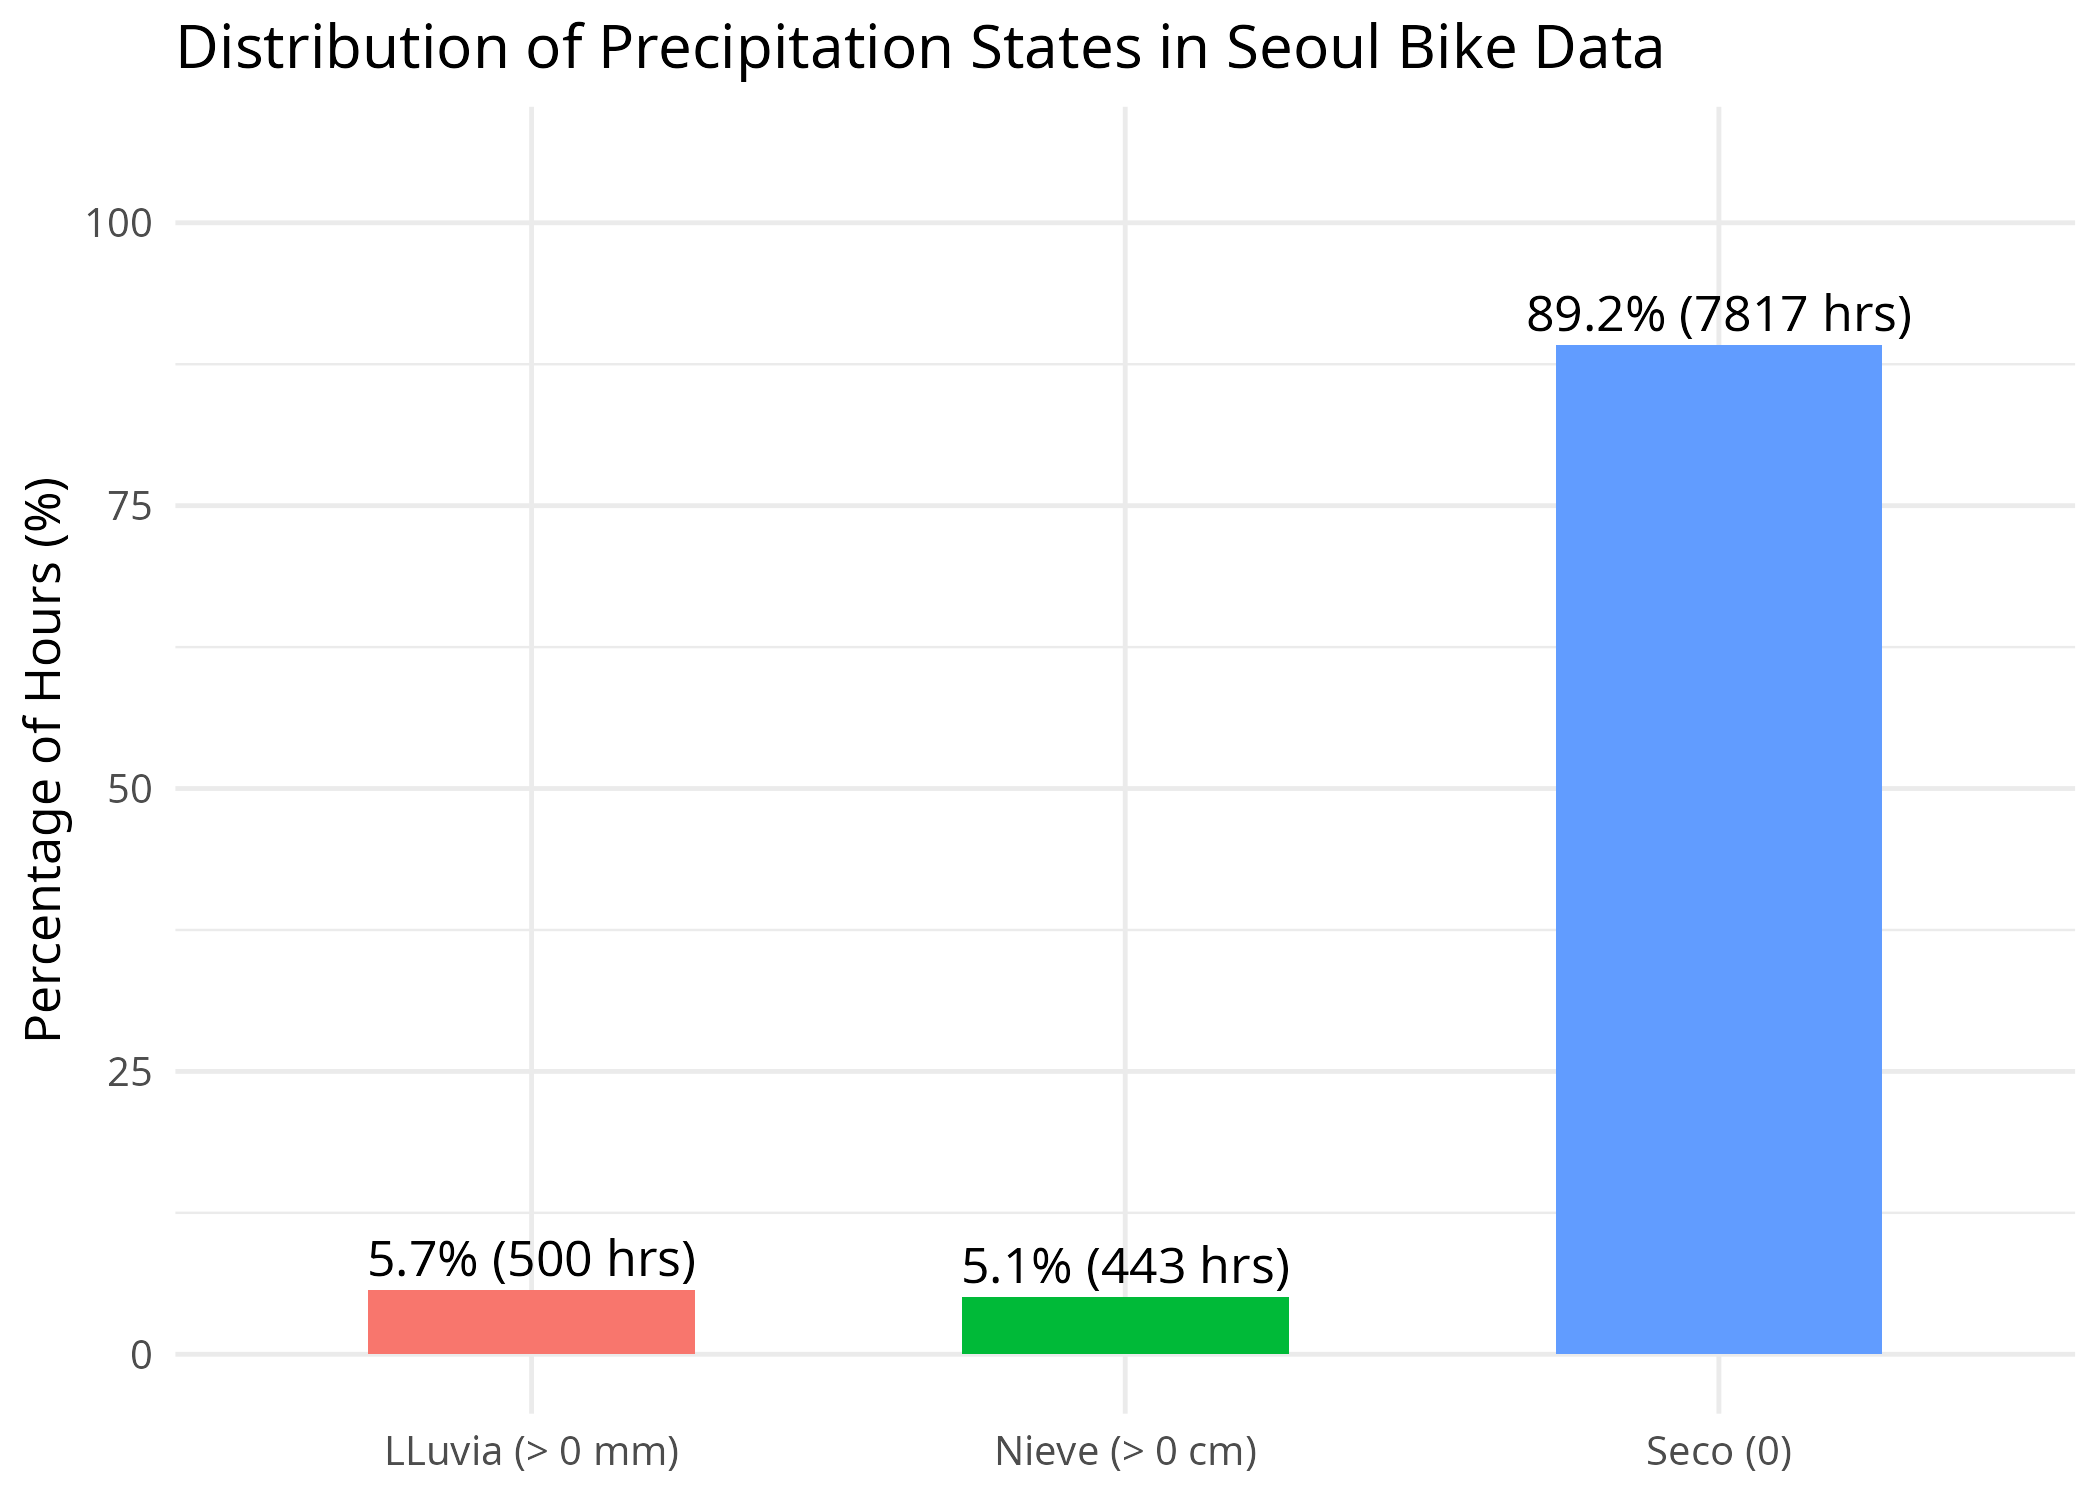
\includegraphics[width=\textwidth]{plots/01_eda_estados_precipitacion.png}
        \caption{Estados de precipitación en la base original ($n = 8\,760$).}
        \label{fig:precipitacion}
    \end{subfigure}
    \hfill
    \begin{subfigure}[b]{0.8\textwidth}
        \centering
        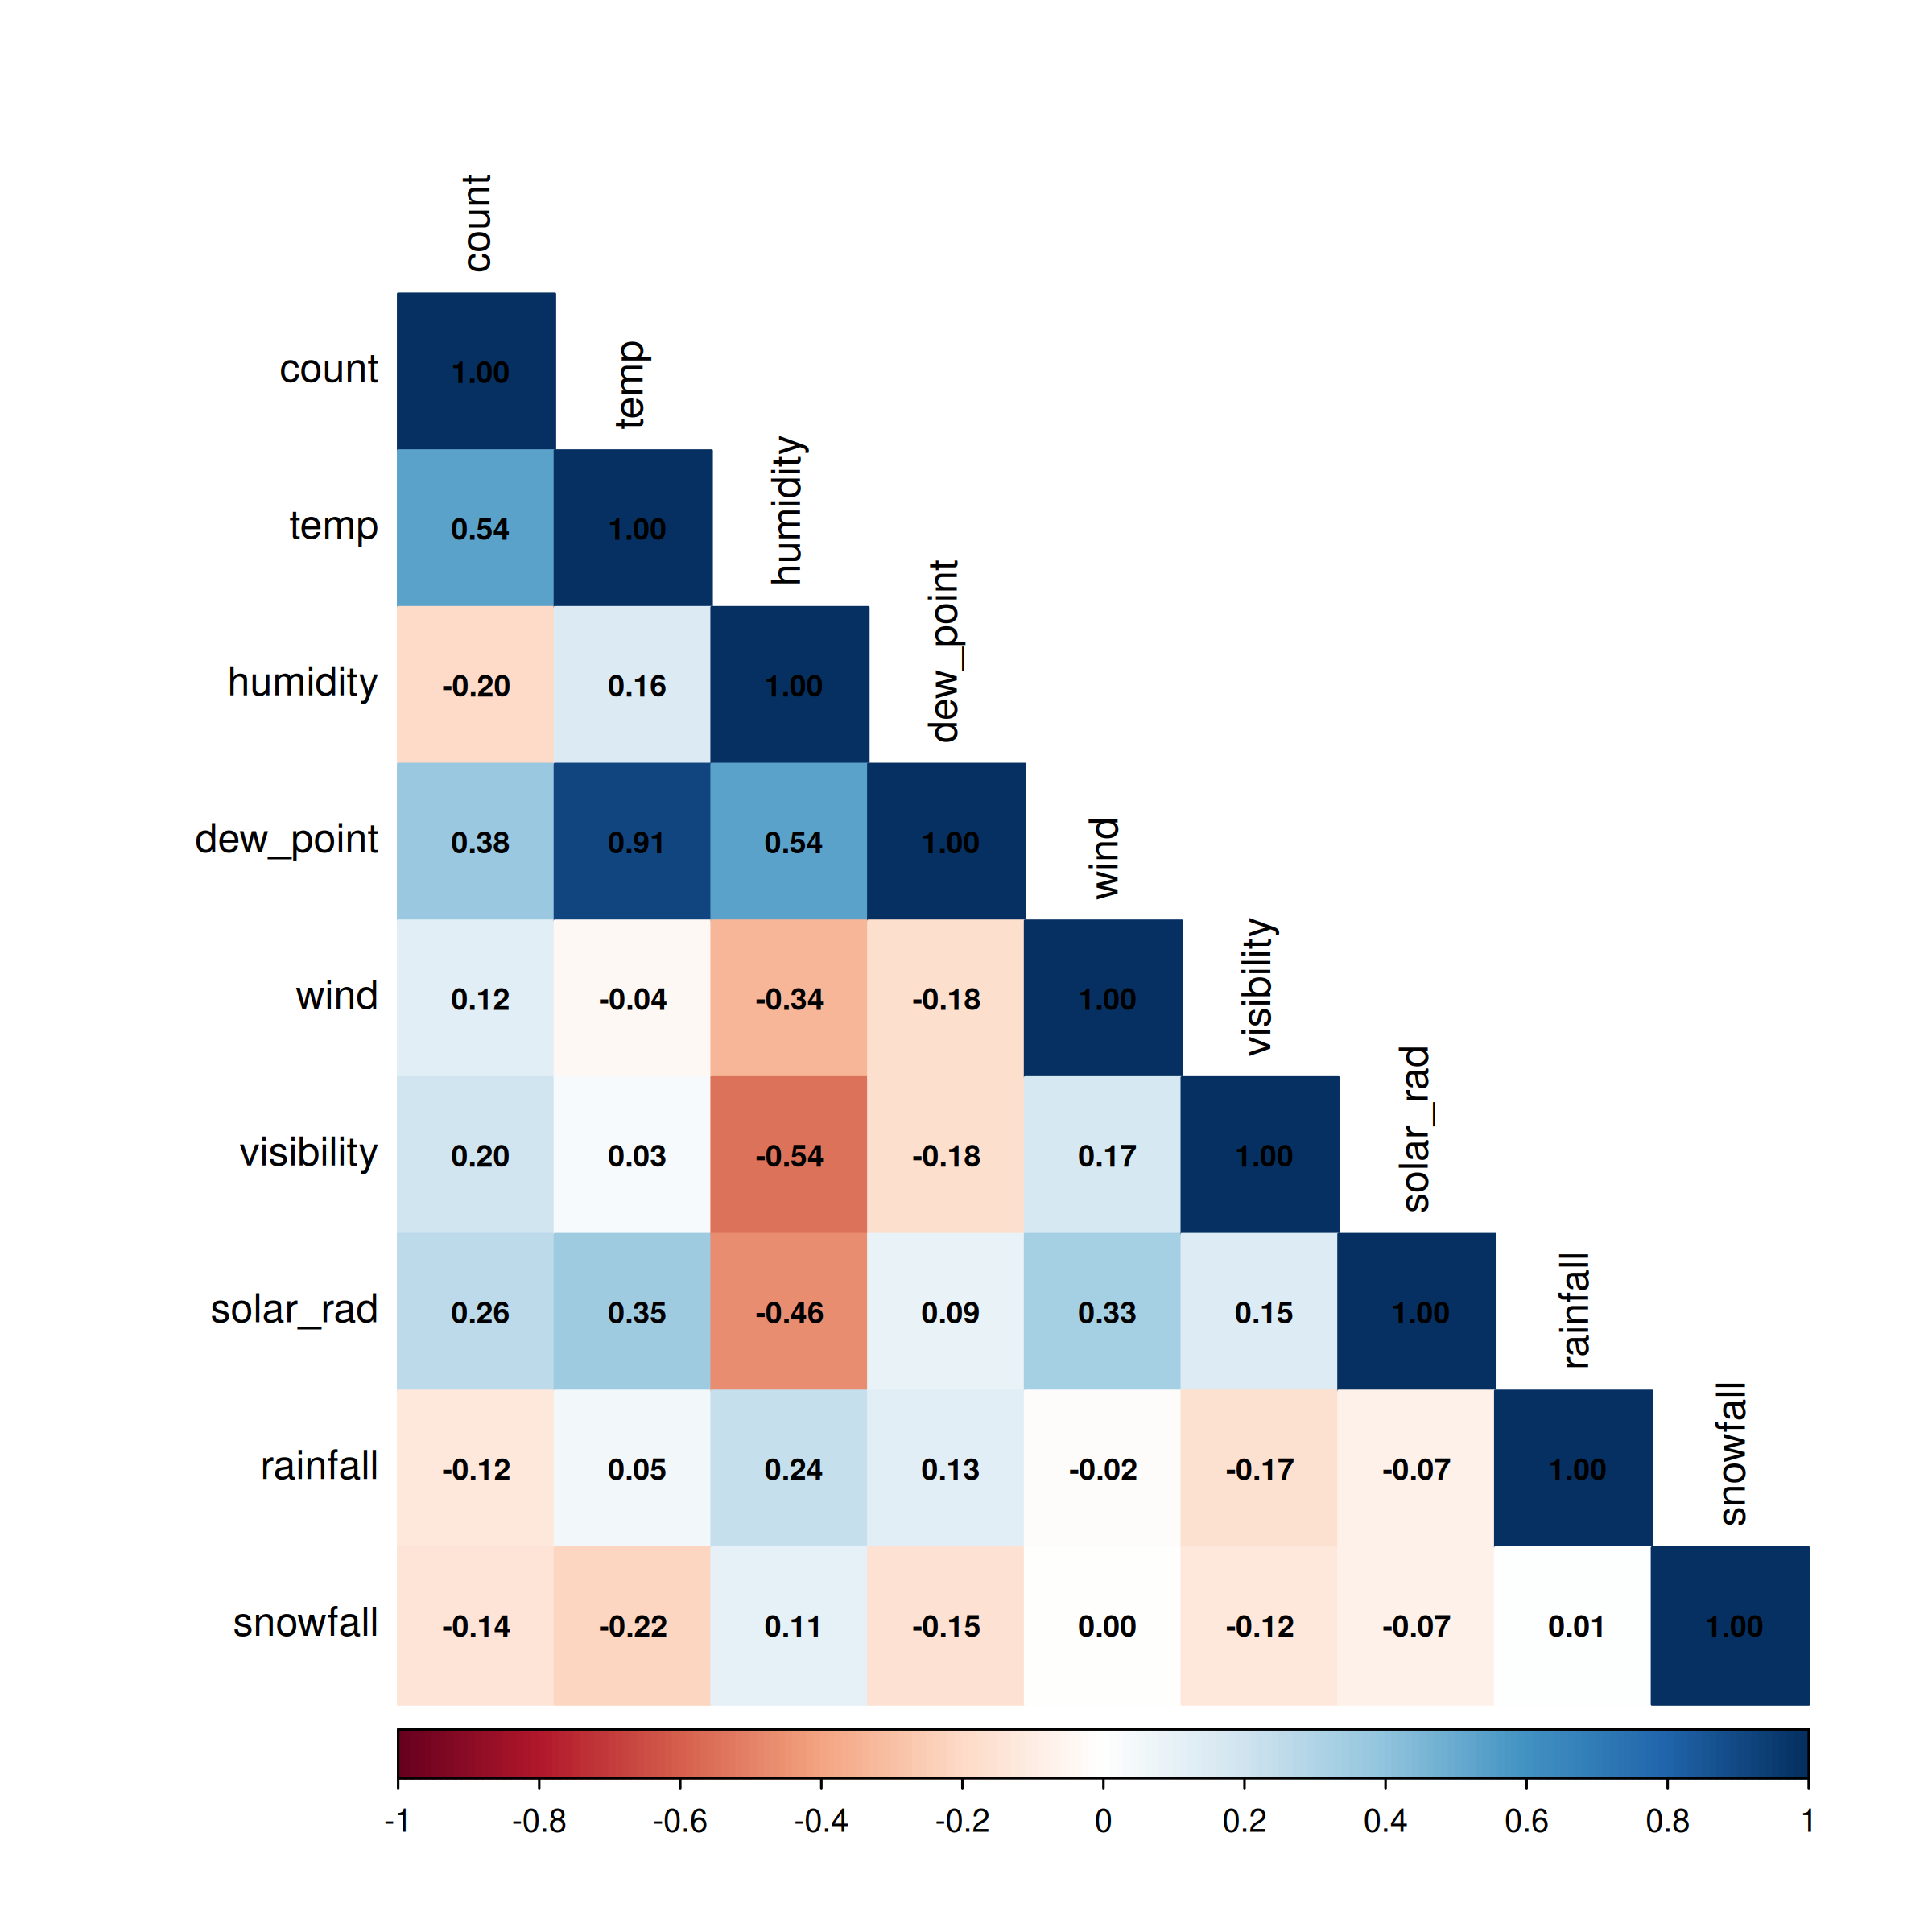
\includegraphics[width=\textwidth]{plots/01_eda_matriz_correlacion.png}
        \caption{Matriz de correlaciones de Pearson.}
        \label{fig:correlaciones}
    \end{subfigure}
    \caption{Justificación del preprocesamiento de variables meteorológicas.}
    \label{fig:preprocesamiento}
\end{figure}

Debido a la gran proporción de horas sin precipitaciones (Figura~\ref{fig:precipitacion}), las variables lluvia y nieve fueron redefinidas como variables indicadoras según la presencia (valor 1) o ausencia (valor 0). Esta redefinición permite comparar las horas con y sin precipitaciones sin distinguir su intensidad.

La hora del día se consideró como variable categórica, pues no se espera una relación lineal entre la hora y la demanda.

La base original no incluye el día de la semana, por lo que esta variable se construyó a partir de la fecha de cada registro. Se definió como una variable categórica de siete niveles, de lunes a domingo, con el lunes como categoría de referencia. Su inclusión permite distinguir los patrones de uso de los días hábiles y del fin de semana, que no quedan recogidos por la variable feriado.
\begin{table}[htbp]
\centering\small
\caption{Variables consideradas en el análisis de regresión.}
\begin{adjustbox}{max width=\linewidth}
\begin{tabular}{lll}
\toprule
Variable & Tipo & Rango, categoría o unidad \\
\midrule
Arriendos por hora & Conteo & $2$--$3556$ bicicletas \\
Hora & Categórica & 0, 1, $\ldots$, 23 \\
Temperatura & Continua & $-17{,}8$ a $39{,}4$ $^\circ$C \\
Humedad relativa & Continua & 0--98 (\%) \\
Velocidad del viento & Continua & 0--7{,}4 (m/s) \\
Visibilidad & Continua & 27--2000 (unidades de 10 m) \\
Radiación solar & Continua & 0--3{,}52 (MJ/m$^2$) \\
Estación & Categórica & Otoño, primavera, verano, invierno \\
Feriado & Categórica & Sí, no \\
Día de la semana & Categórica & Lunes, martes, $\ldots$, domingo \\
Lluvia & Binaria & Presencia o ausencia \\
Nieve & Binaria & Presencia o ausencia \\
\bottomrule
\end{tabular}
\end{adjustbox}
\end{table}

\newpage
\subsection{Análisis exploratorio}

A continuación, se presentan los principales estadísticos
descriptivos de las variables consideradas en el estudio. En particular, se incluyen medidas de tendencia central y
dispersión para las variables cuantitativas, junto con la
distribución de las observaciones y además se presenta la demanda promedio de
bicicletas según las diferentes categorías de las variables
cualitativas.

\begin{table}[htbp]
\centering
\small
\caption{Estadísticos descriptivos de las variables cuantitativas.}
\begin{adjustbox}{max width=\linewidth}
\begin{tabular}{lrrrrr}
\toprule
Variable & Media & DE & Mín. & Mediana & Máx. \\
\midrule
Bicicletas arrendadas & 729{,}16 & 642{,}35 & 2 & 542 & 3556 \\
Temperatura & 12{,}77 & 12{,}10 & $-$17{,}8 & 13{,}5 & 39{,}4 \\
Humedad & 58{,}15 & 20{,}48 & 0 & 57 & 98 \\
Viento & 1{,}73 & 1{,}03 & 0 & 1{,}5 & 7{,}4 \\
Visibilidad & 1433{,}87 & 609{,}05 & 27 & 1690 & 2000 \\
Radiación solar & 0{,}57 & 0{,}87 & 0 & 0{,}01 & 3{,}52 \\
\bottomrule
\end{tabular}
\end{adjustbox}
\label{tab:descriptivos}
\end{table}

\begin{table}[htbp]
\centering
\small
\caption{Demanda promedio por hora según variables categóricas.}
\begin{adjustbox}{max width=\linewidth}
\begin{tabular}{llrr}
\toprule
Variable & Categoría & Observaciones & Media \\
\midrule
Estación & Primavera & 2160 & 746{,}25 \\
         & Verano    & 2208 & 1034{,}07 \\
         & Otoño     & 1937 & 924{,}11 \\
         & Invierno  & 2160 & 225{,}54 \\
\midrule
Feriado  & Sí & 408  & 529{,}15 \\
         & No & 8057 & 739{,}28 \\
\midrule
Lluvia   & Sí & 516  & 167{,}26 \\
         & No & 7949 & 765{,}63 \\
\midrule
Nieve    & Sí & 443  & 185{,}10 \\
         & No & 8022 & 759{,}20 \\
\midrule
Día de la semana & Lunes     & 1248 & 730{,}56 \\
                 & Martes    & 1152 & 745{,}31 \\
                 & Miércoles & 1200 & 769{,}96 \\
                 & Jueves    & 1200 & 718{,}33 \\
                 & Viernes   & 1224 & 776{,}42 \\
                 & Sábado    & 1217 & 727{,}60 \\
                 & Domingo   & 1224 & 637{,}41 \\
\bottomrule
\end{tabular}
\end{adjustbox}
\label{tab:categoricas}
\end{table}

%%\begin{table}[htbp]
%\centering
%\small
%\caption{Diagnóstico del modelo cuasi-Poisson.}
%\begin{tabular}{lcr}
%\toprule
%Criterio & Umbral & Observaciones \\
%\midrule
%Residuo de Pearson estandarizado & $|r_i^*|>3$ & 65 \\
%Apalancamiento & $h_{ii}>2p/n$ & 166 \\
%Distancia de Cook & $D_i>4/n$ & 659 \\
%\bottomrule
%\end{tabular}
%\label{tab:diagnostico}
%%\end{table}

En la muestra se observa que la cantidad de bicicletas arrendadas por hora presenta una media de 729{,}16, una mediana de 542 y una desviación estándar de 642{,}35.

Los cuartiles primero y tercero corresponden a 214 y 1084 bicicletas, respectivamente, lo que evidencia una considerable variabilidad de la demanda.

Las horas de mayor demanda promedio corresponden a las 18:00 (1554 arriendos) y las 19:00 (1236 arriendos), mientras que la menor demanda se registra a las 04:00 (137 arriendos).
\newpage
$\\$
Por estación, los promedios son 1034 en verano, 924 en otoño, 746 en primavera y 226 en invierno.
En presencia de lluvia, se registran en promedio 167 arriendos por hora, frente a 766 en ausencia de lluvia.
Según el día de la semana, la demanda promedio es similar de lunes a sábado (entre 718 y 776 arriendos por hora) y disminuye el domingo, con 637 arriendos por hora. Las diferencias entre días son menores que las observadas entre horas del día, lo que sugiere que el día de la semana influye principalmente en la forma del perfil horario de la demanda.
Asimismo, la correlación de Pearson entre temperatura y número de arriendos es de $0{,}563$. Estas relaciones son descriptivas y no controlan el efecto de las demás covariables.

\begin{figure}[htbp]
    \centering
    \begin{subfigure}[b]{0.48\textwidth}
        \centering
        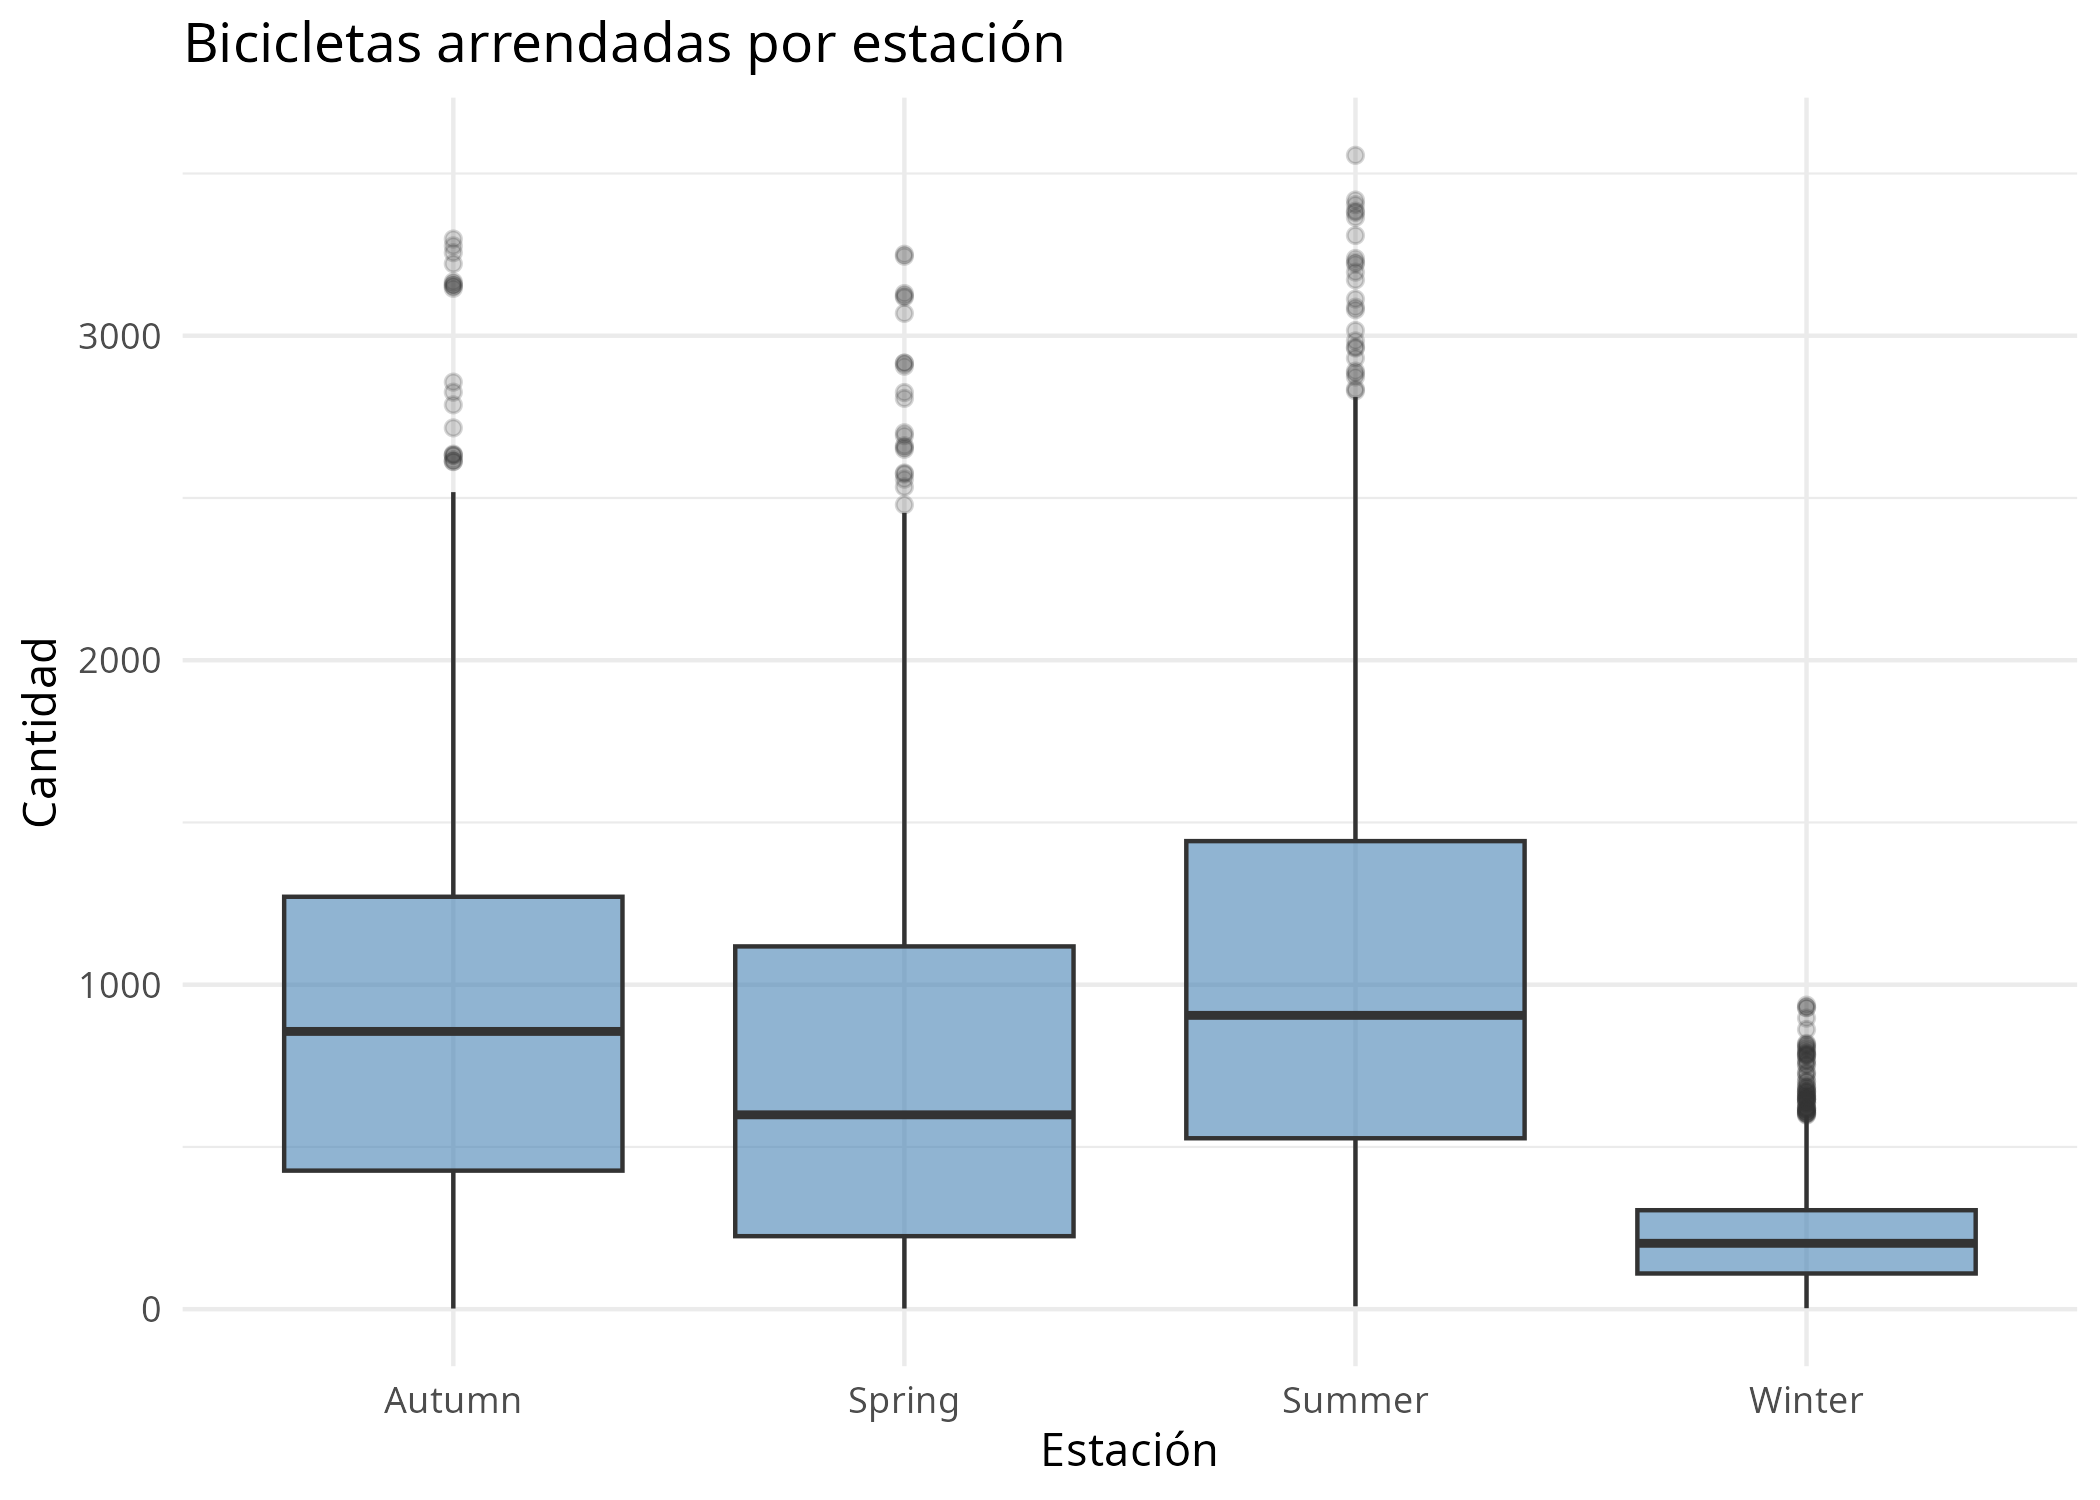
\includegraphics[width=\textwidth]{plots/01_eda_boxplot_estacion.png}
        \caption{Demanda por estación del año.}
        \label{fig:box_estacion}
    \end{subfigure}
    \hfill
    \begin{subfigure}[b]{0.48\textwidth}
        \centering
        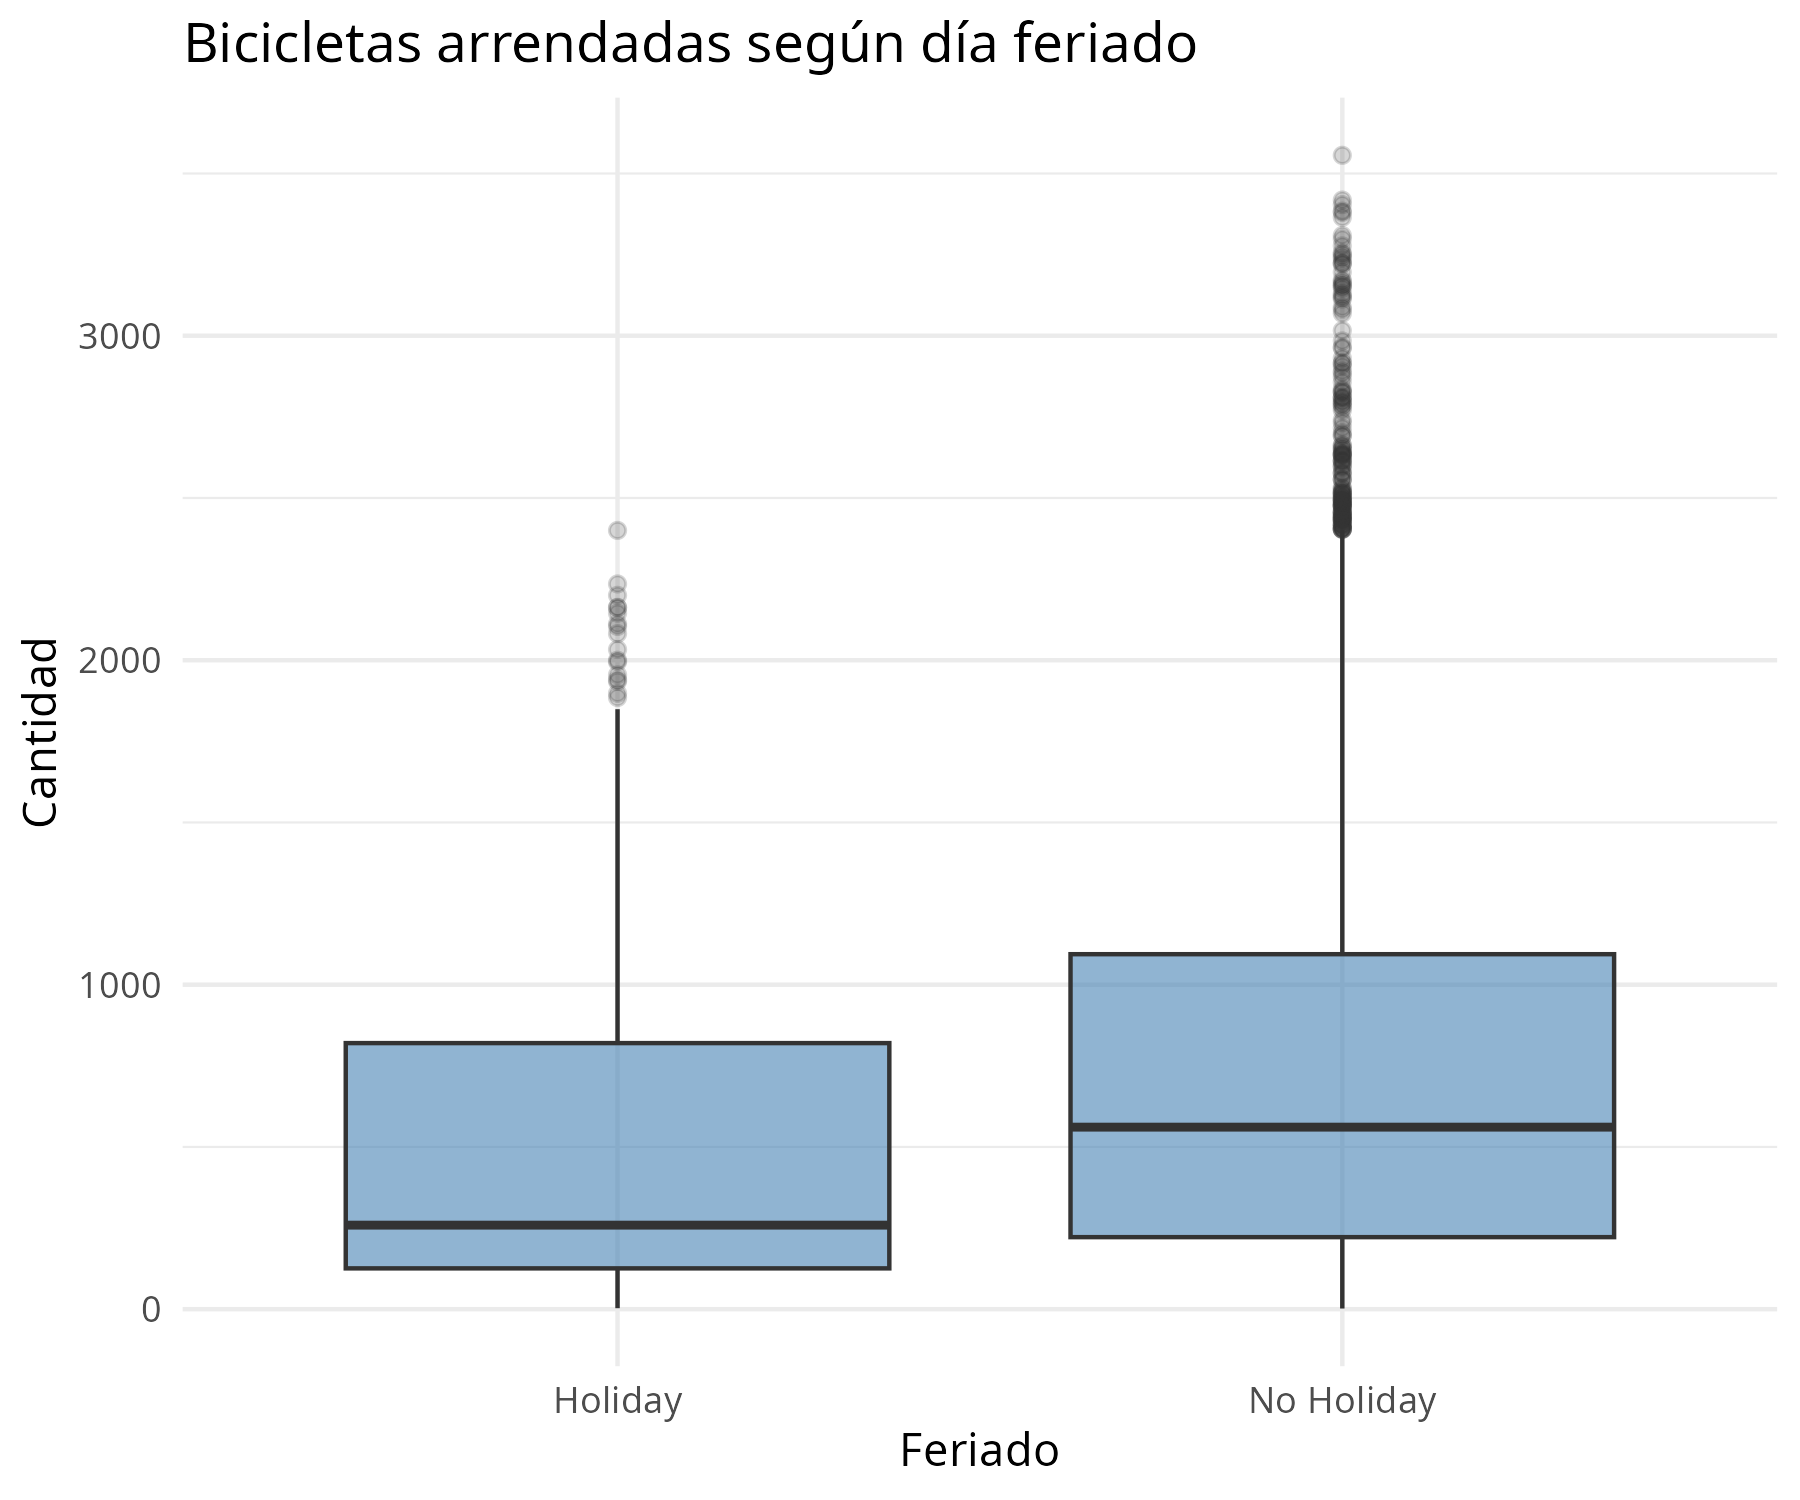
\includegraphics[width=\textwidth]{plots/01_eda_boxplot_feriado.png}
        \caption{Demanda según día feriado.}
        \label{fig:box_feriado}
    \end{subfigure}

    \vspace{0.3cm}

    \begin{subfigure}[b]{0.48\textwidth}
        \centering
        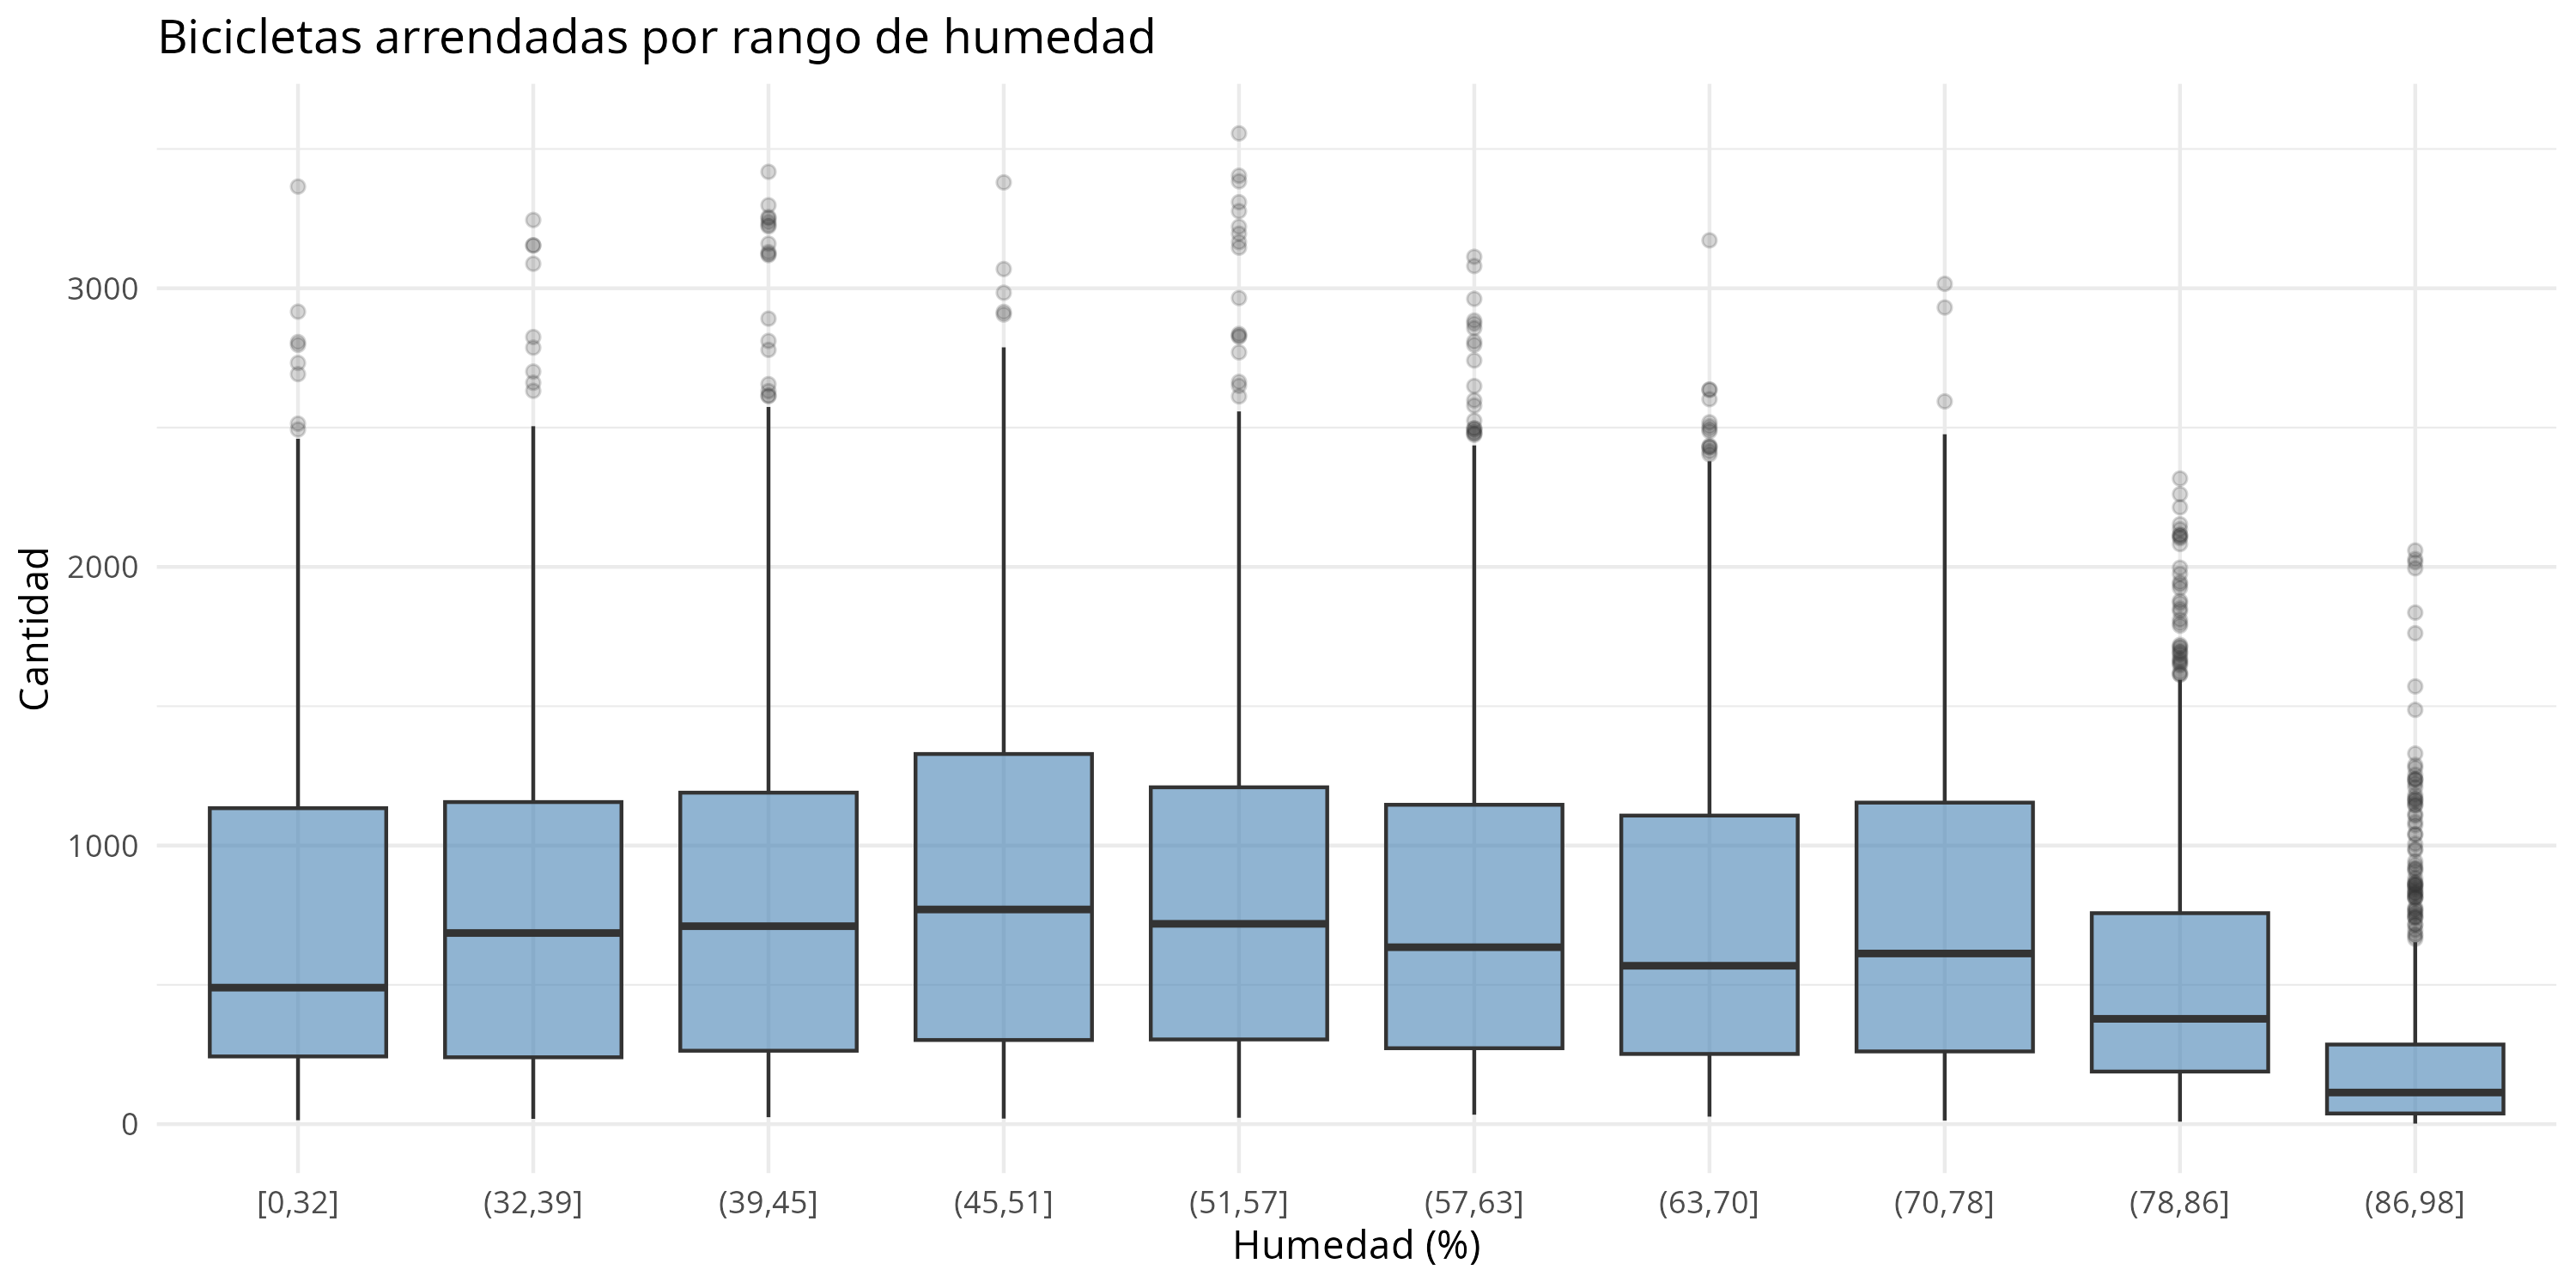
\includegraphics[width=\textwidth]{plots/01_eda_boxplot_humedad.png}
        \caption{Demanda por deciles de humedad.}
        \label{fig:box_humedad}
    \end{subfigure}
    \hfill
    \begin{subfigure}[b]{0.48\textwidth}
        \centering
        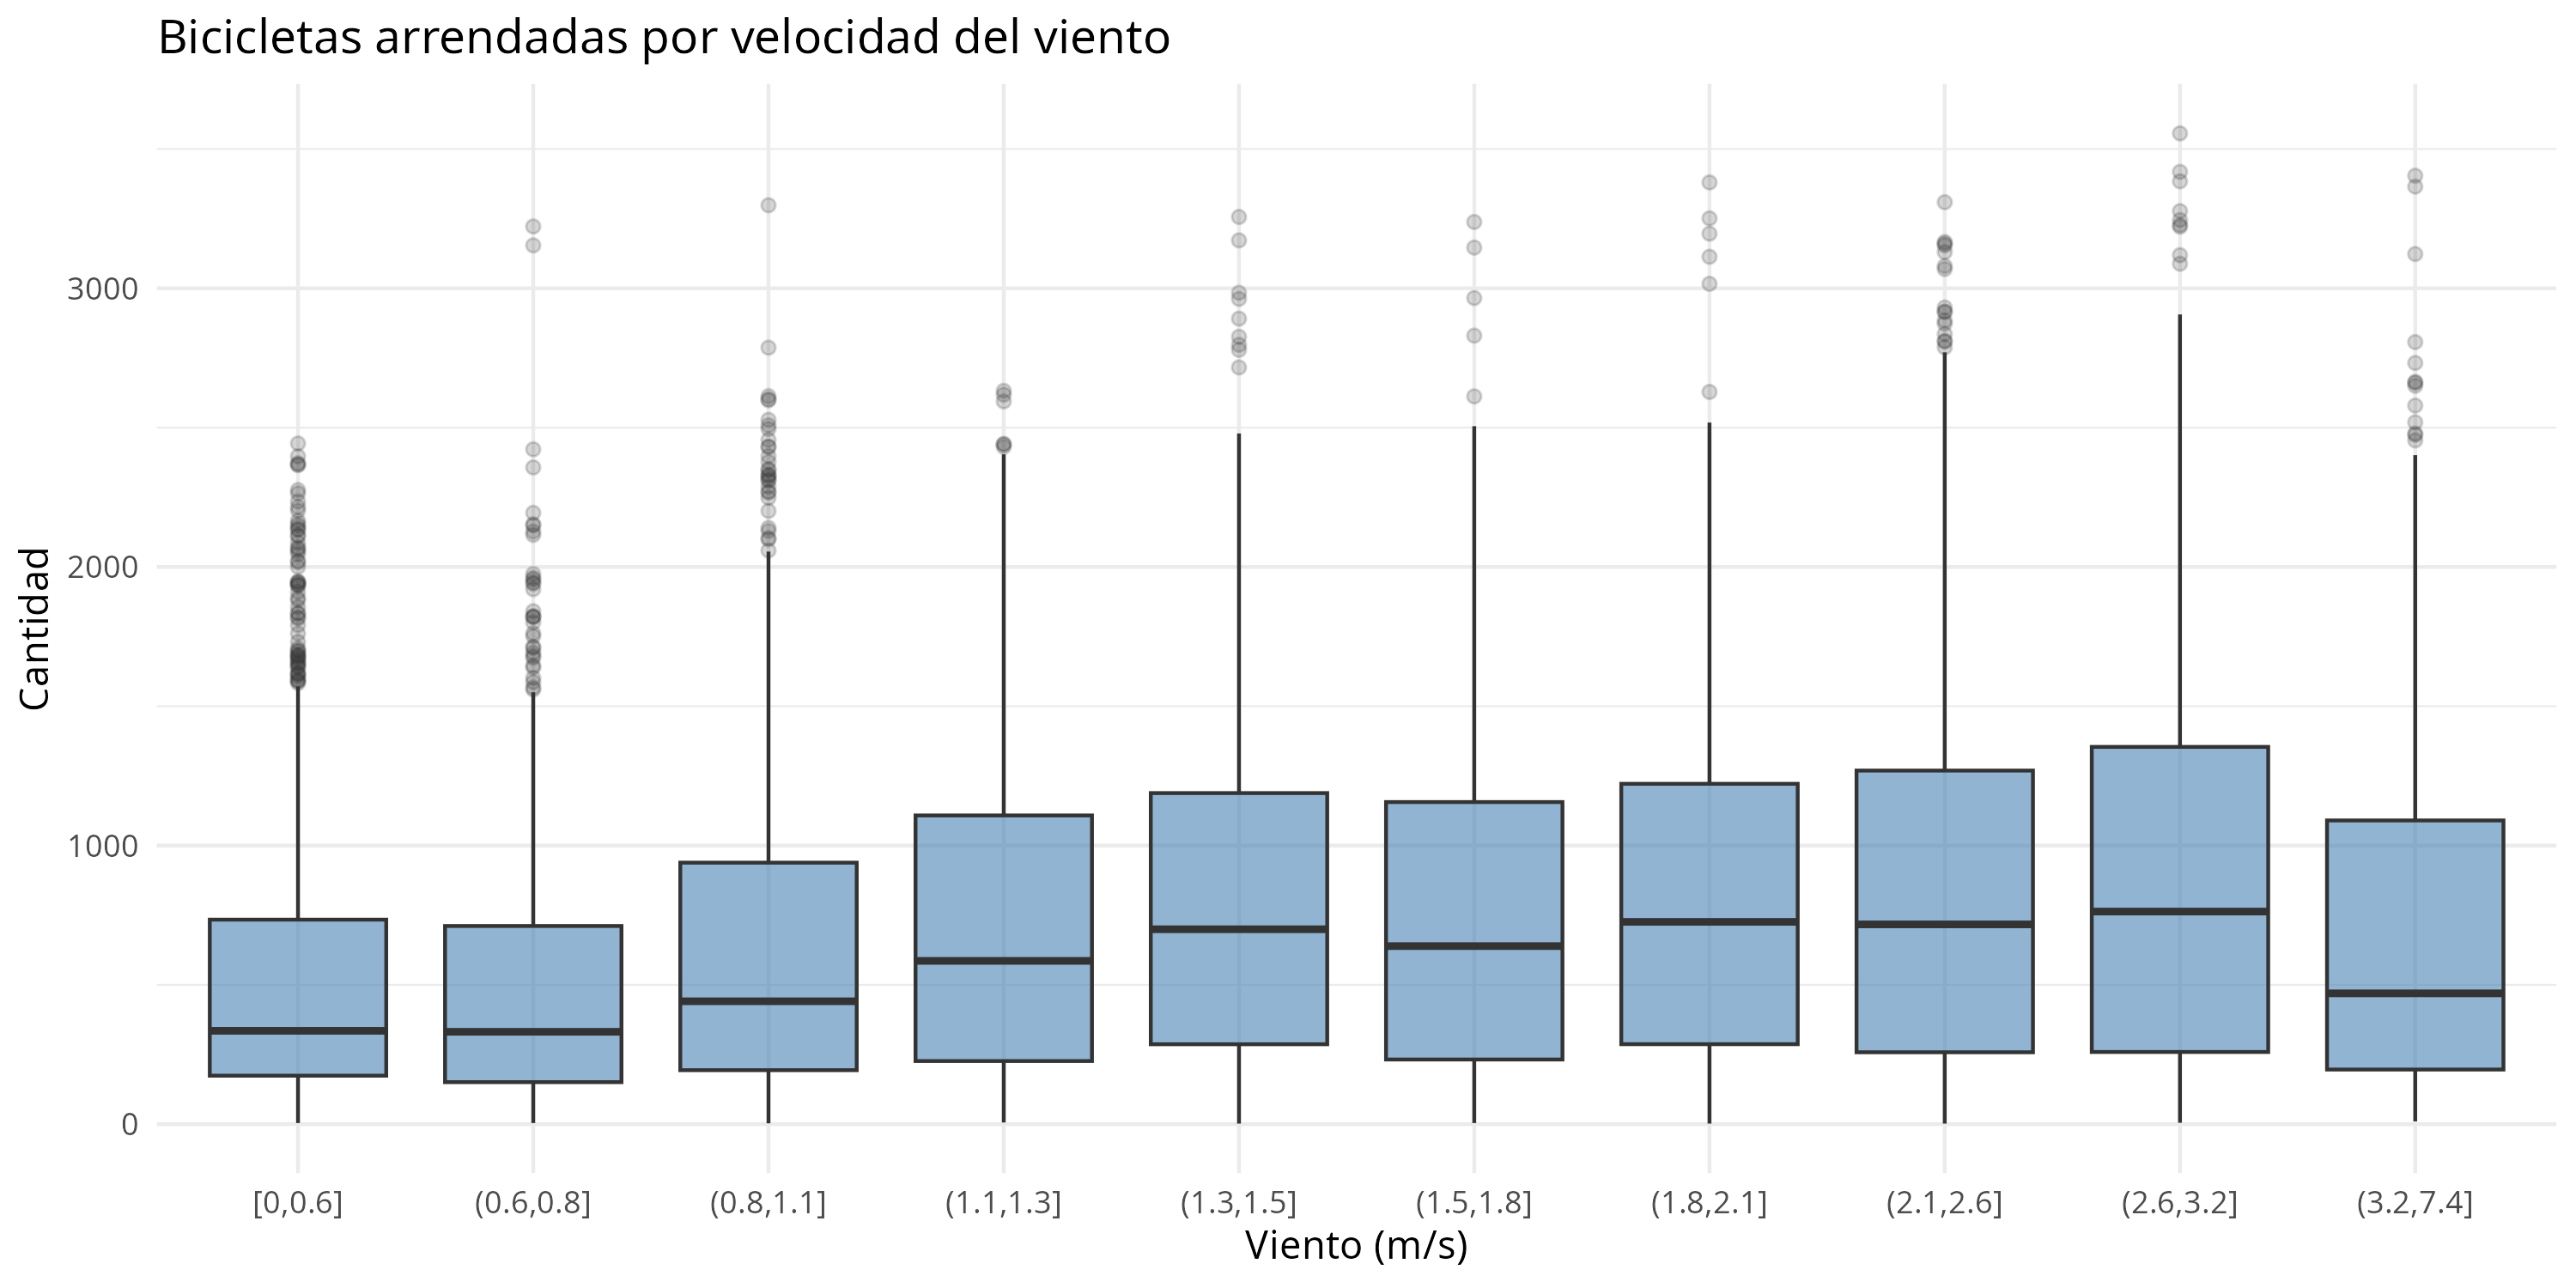
\includegraphics[width=\textwidth]{plots/01_eda_boxplot_viento.png}
        \caption{Demanda por deciles de velocidad del viento.}
        \label{fig:box_viento}
    \end{subfigure}

    \begin{subfigure}[b]{0.48\textwidth}
        \centering
        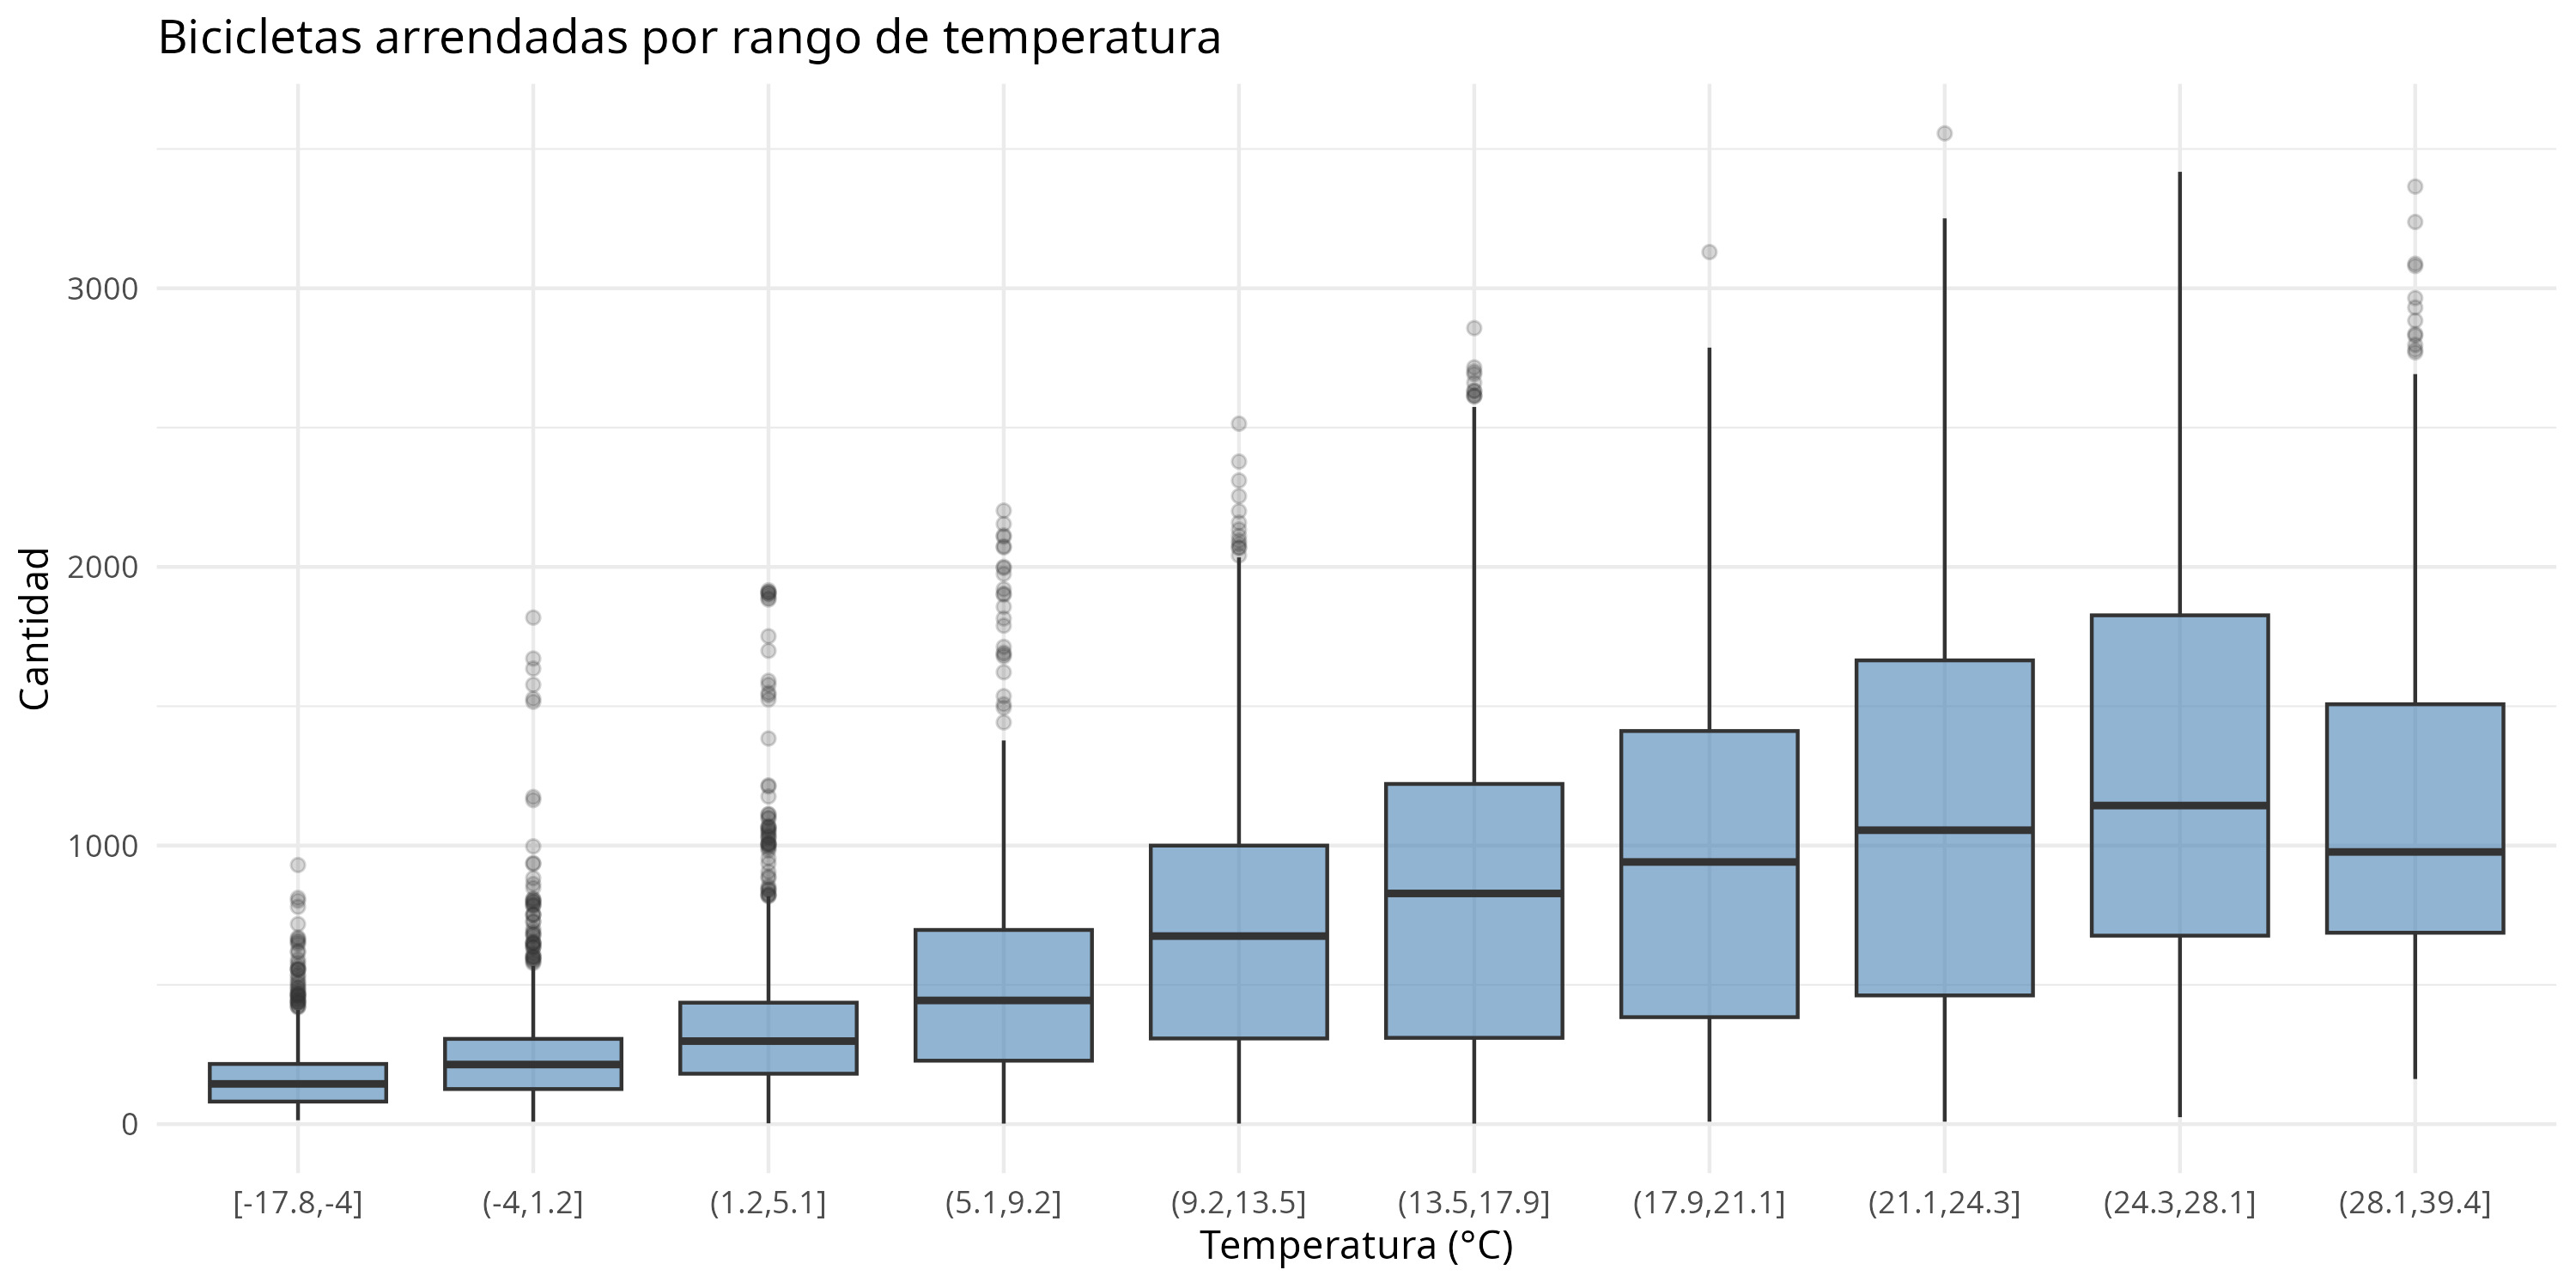
\includegraphics[width=\textwidth]{plots/01_eda_boxplot_temperatura.png}
        \caption{Demanda por rangos de temperatura}
        \label{fig:box_temp}
    \end{subfigure}
    \begin{subfigure}[b]{0.48\textwidth}
        \centering
        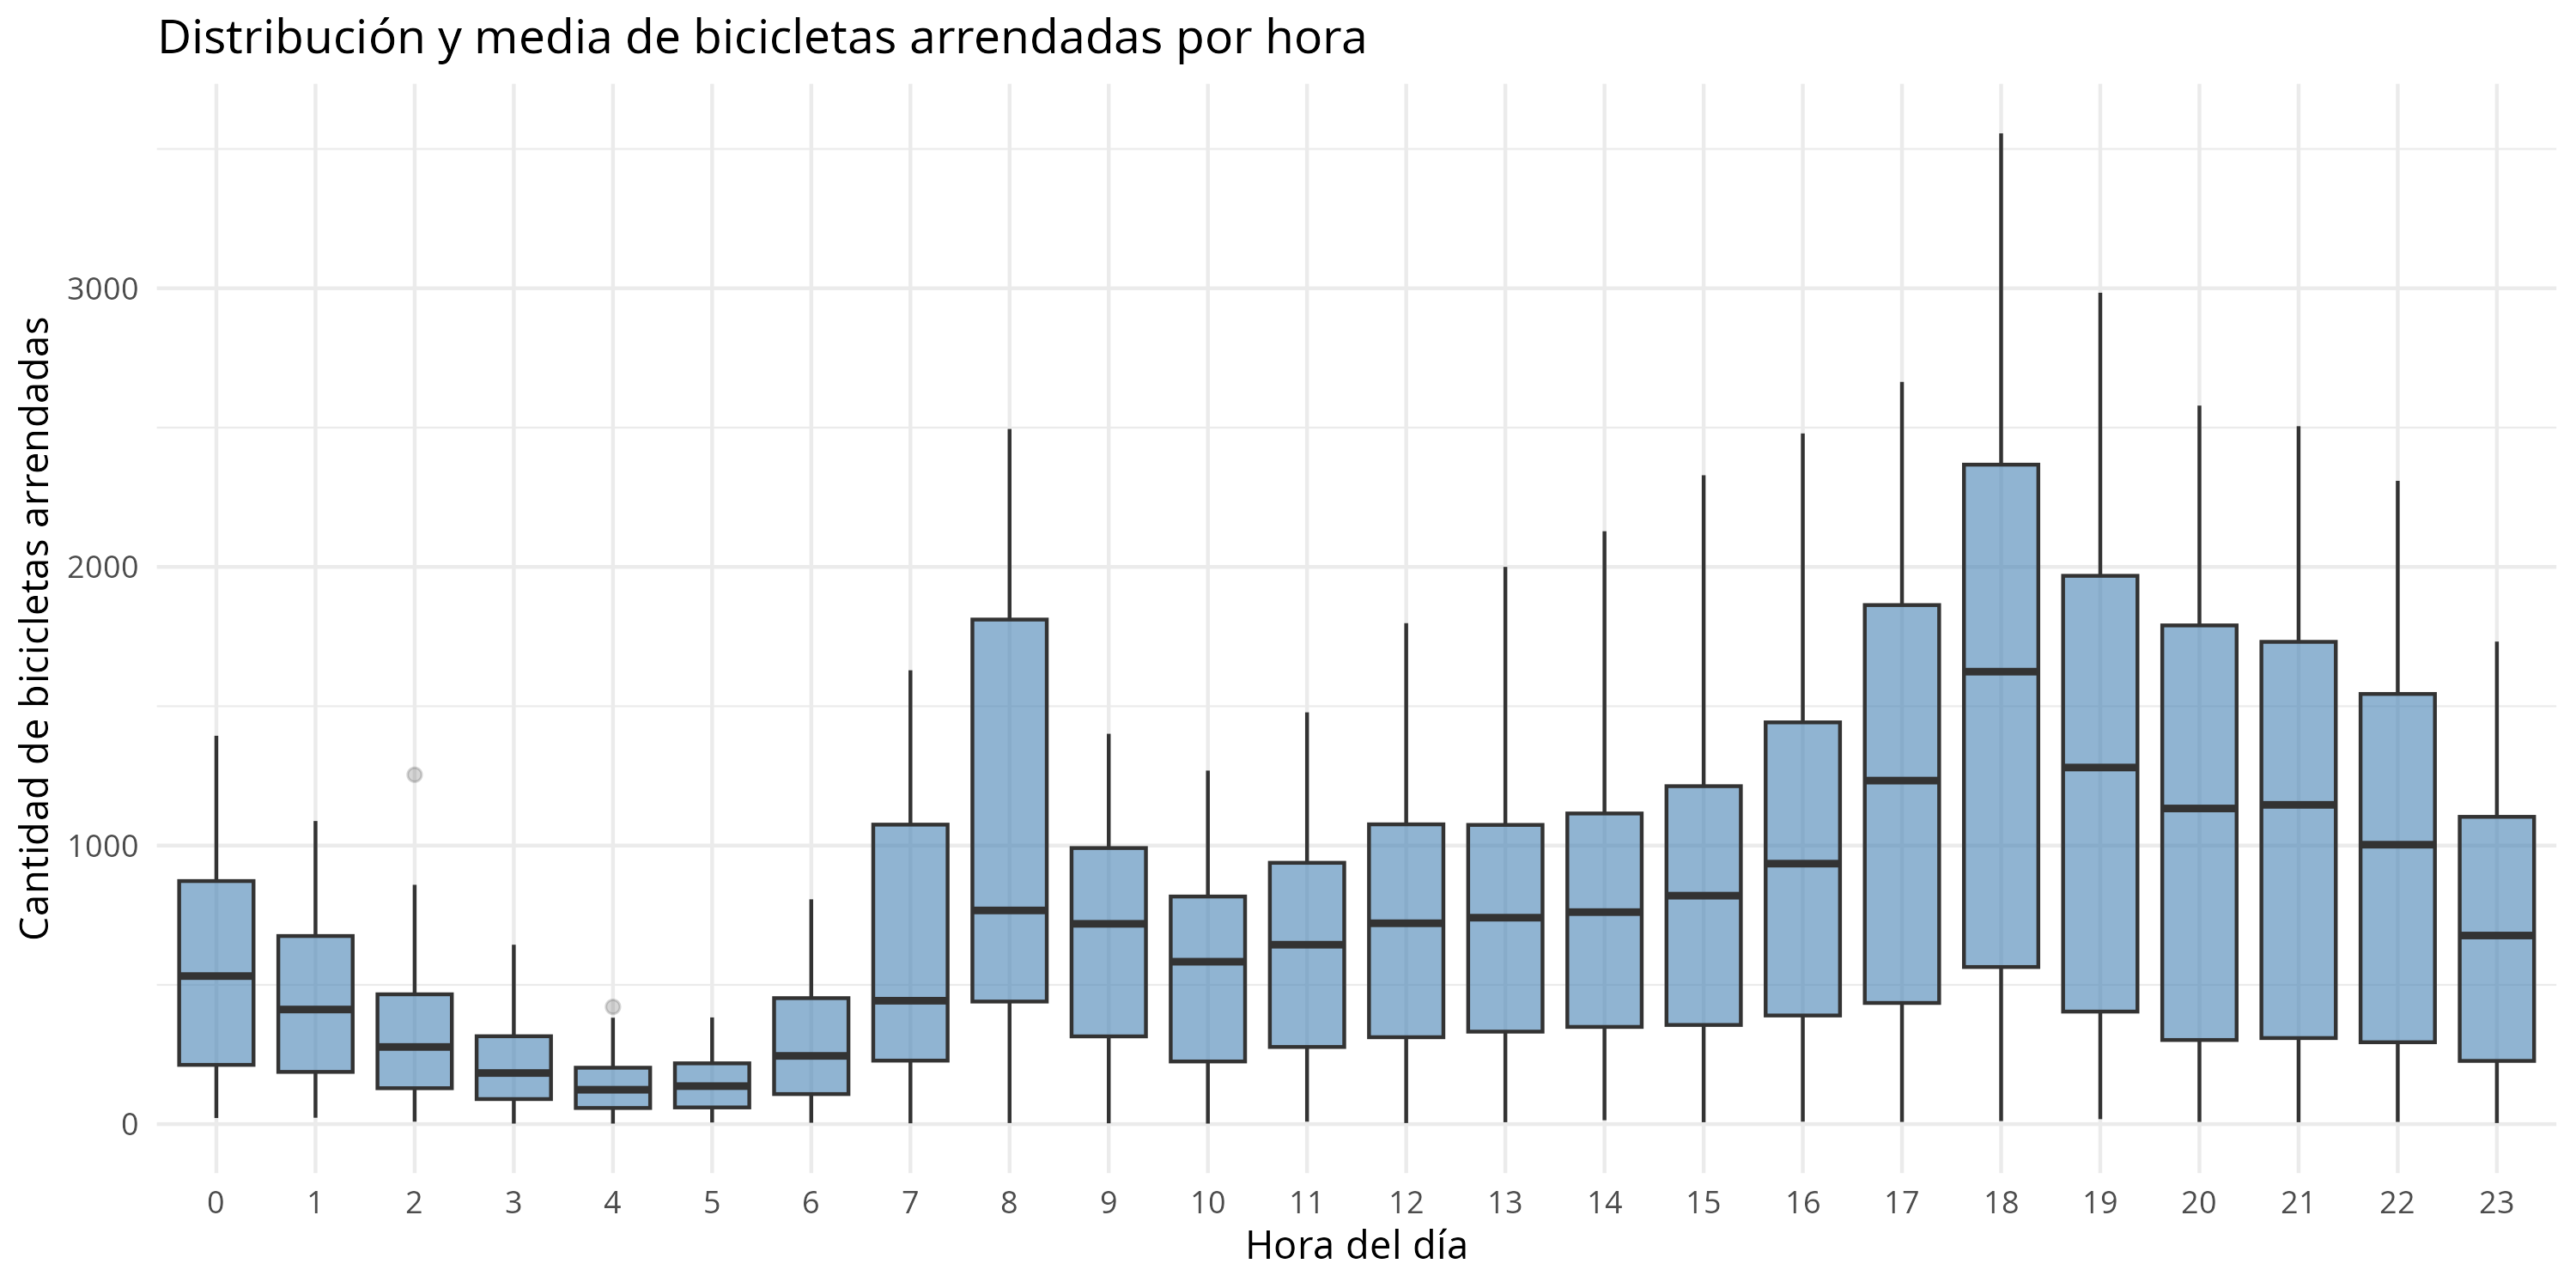
\includegraphics[width=\textwidth]{plots/01_eda_boxplot_hora.png}
        \caption{Demanda por hora del día.}
        \label{fig:box_hora}
    \end{subfigure}

    \vspace{0.3cm}

    \begin{subfigure}[b]{0.48\textwidth}
        \centering
        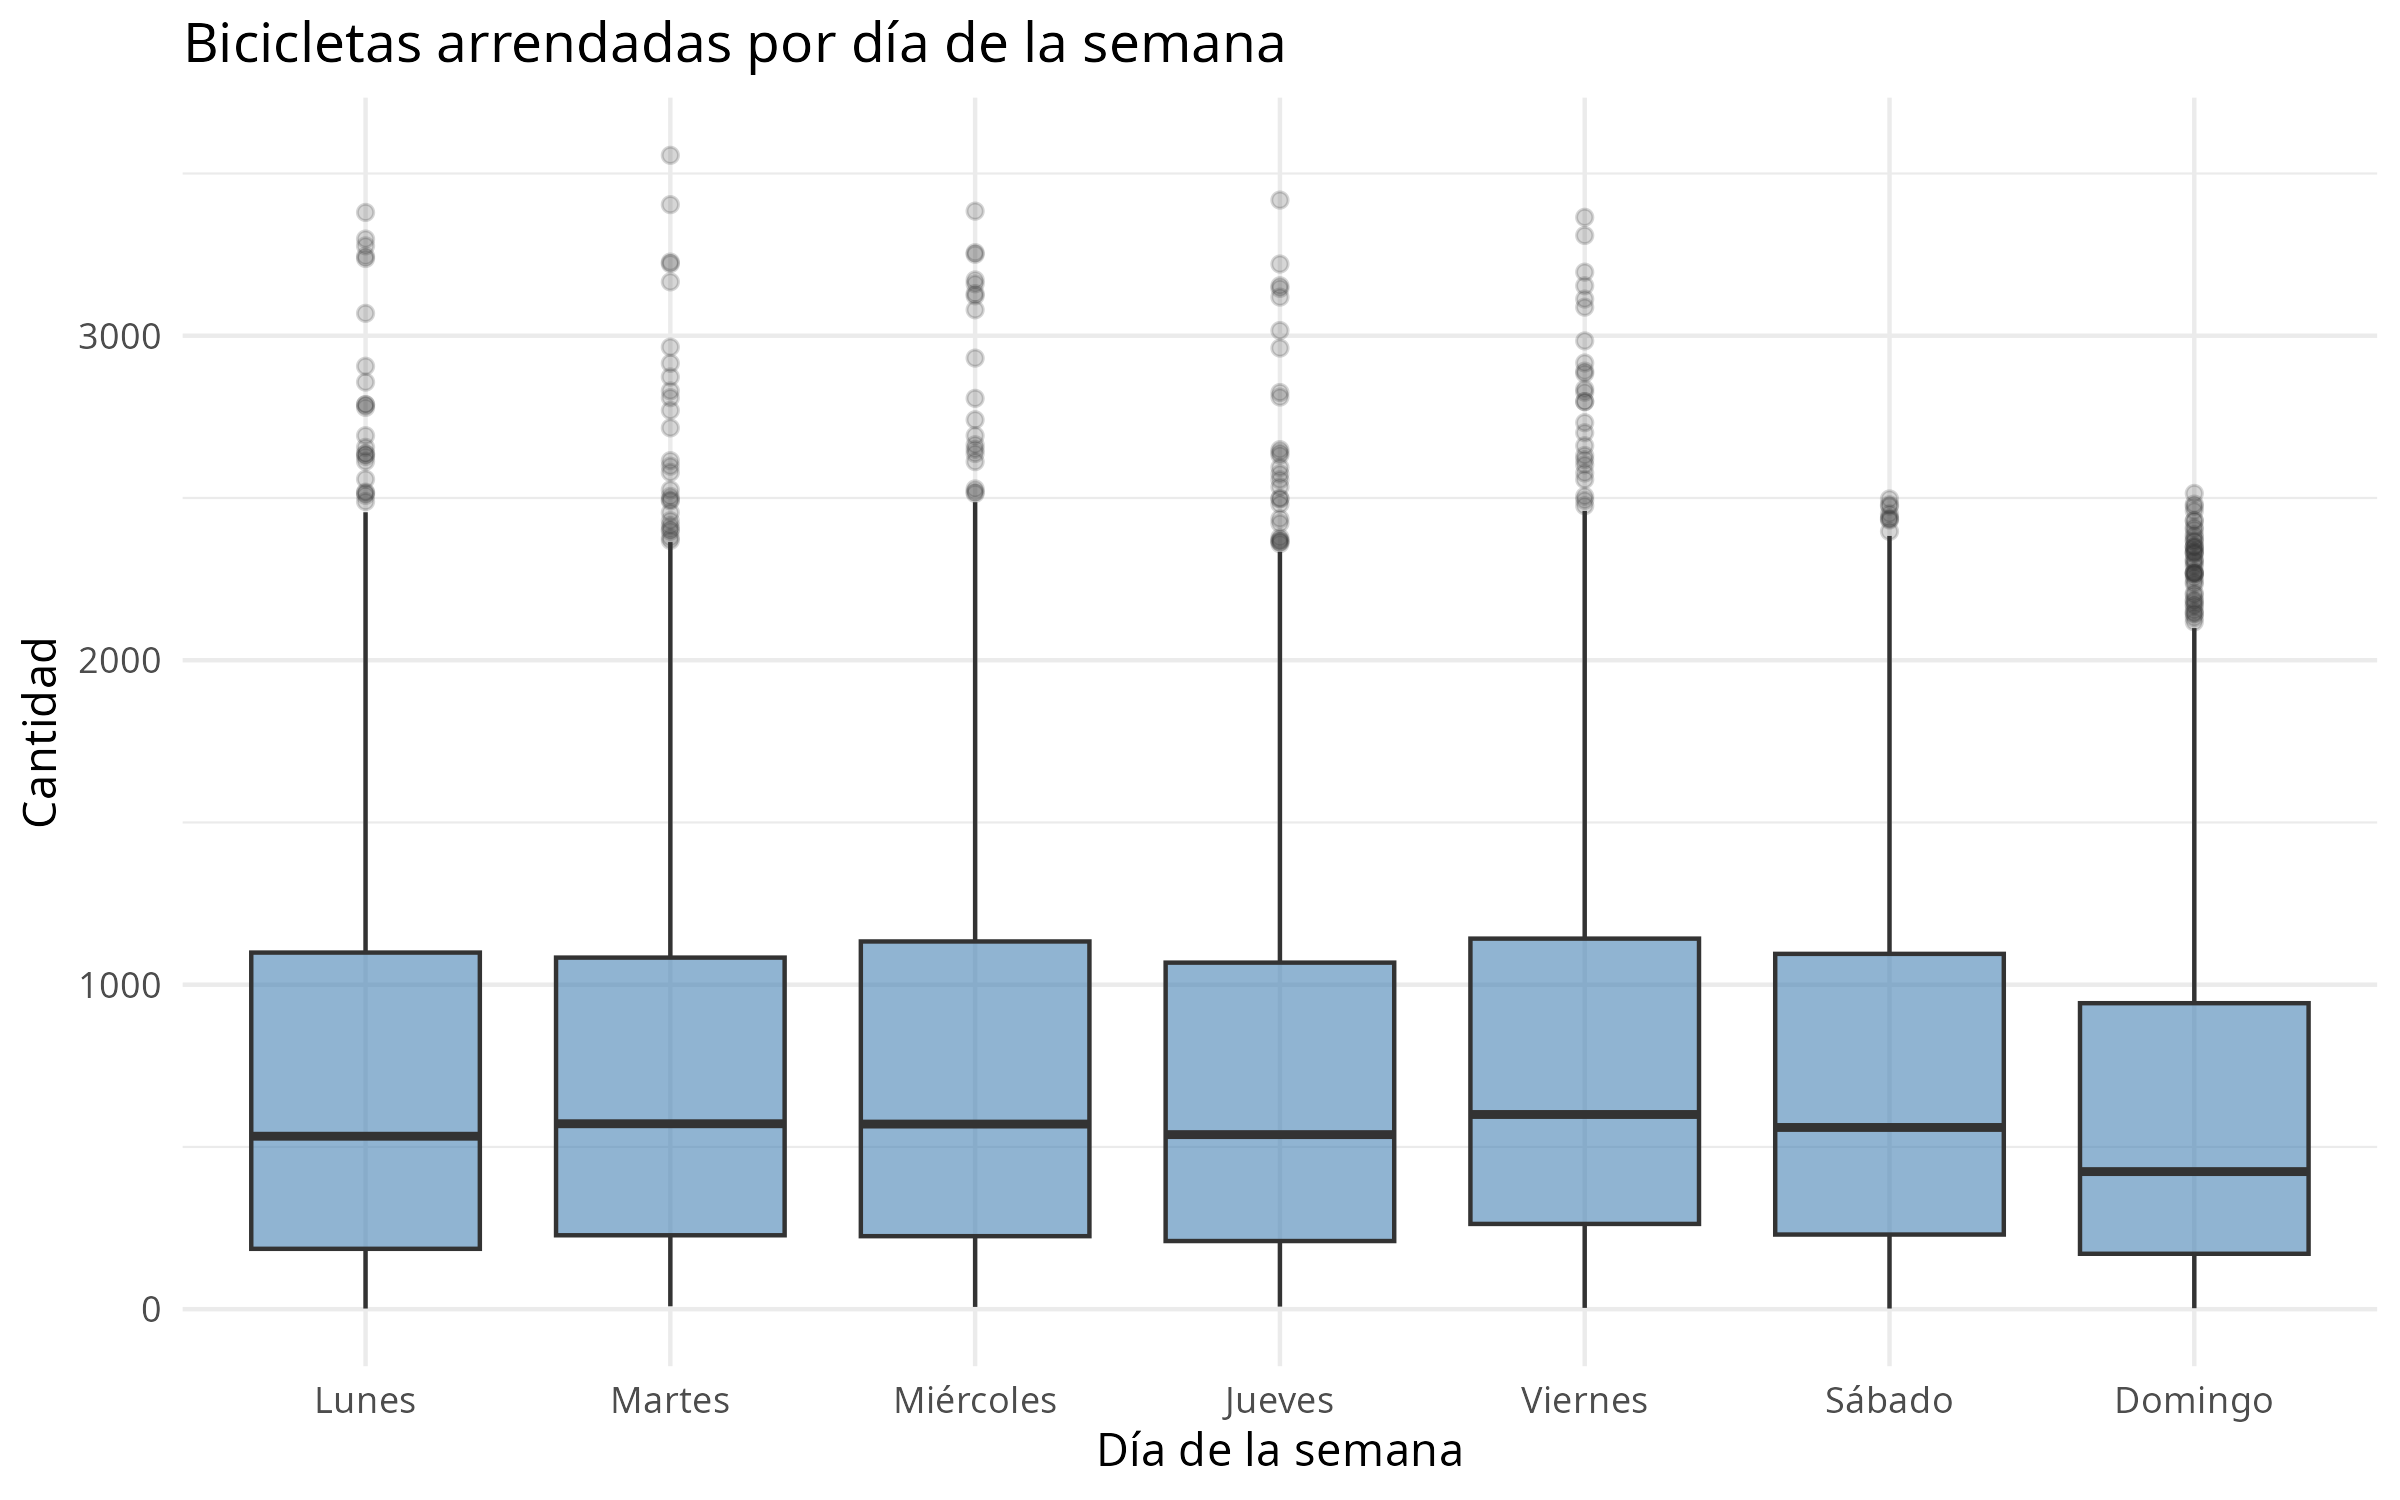
\includegraphics[width=\textwidth]{plots/01_eda_boxplot_dia_semana.png}
        \caption{Demanda por día de la semana.}
        \label{fig:box_dia_semana}
    \end{subfigure}
    \caption{Distribución de la demanda horaria de bicicletas según factores temporales y climáticos.}
    \label{fig:eda_boxplots}


\end{figure}
\newpage

\FloatBarrier
\section{Metodología}

\subsection{Justificación del modelo}
Sea $Y_i$ el número de bicicletas arrendadas durante la $i$-ésima hora de funcionamiento. Dado que $Y_i$ es una variable de conteo discreta y no negativa, se consideró inicialmente un modelo de regresión Poisson con enlace logarítmico, el cual supone condicionalmente que:
\[
Y_i\sim\operatorname{Poisson}(\mu_i),\qquad
\operatorname{E}(Y_i\mid\mathbf{x}_i)=\operatorname{Var}(Y_i\mid\mathbf{x}_i)=\mu_i.
\]

Para evaluar el supuesto de equidispersión se utilizó el estadístico de dispersión de Pearson \cite{mccullagh},
\[
\widehat{\phi}=\frac{X_P^2}{n-p},\qquad
X_P^2=\sum_{i=1}^n\frac{(y_i-\widehat{\mu}_i)^2}{\widehat{\mu}_i},
\]
donde valores $\widehat{\phi}>1$ indican sobredispersión respecto al modelo Poisson. En el modelo aditivo inicial se obtuvo $X_P^2 = 883\,646{,}6$ con $8\,424$ grados de libertad residuales, de modo que $\widehat{\phi}=104{,}90$. Por tanto, el supuesto de equidispersión del modelo Poisson no resulta adecuado.

En base a lo anterior, se consideraron como alternativas los modelos cuasi-Poisson y binomial negativo, cuyas estructuras de varianza son \cite{verhoef}:
\begin{align*}
\text{Cuasi-Poisson:}\qquad &\operatorname{Var}(Y_i\mid\mathbf{x}_i)=\phi\mu_i,\\
\text{Binomial negativa:}\qquad &\operatorname{Var}(Y_i\mid\mathbf{x}_i)=\mu_i+\frac{\mu_i^2}{\theta},
\end{align*}
con $\phi>0$ y $\theta>0$. El modelo cuasi-Poisson conserva la estructura de la media del modelo Poisson, pero permite estimar la dispersión y ajustar los errores estándar de las estimaciones mediante cuasi-verosimilitud \cite{mccullagh}.

\newpage

\subsection{Cuasi-verosimilitud}
La cuasiverosimilitud no exige conocer la función de probabilidad de la variable respuesta.
Para su formulación basta especificar los dos primeros momentos condicionales:
Se postula una media $\mu_i=\mathbb E(Y_i\mid\mathbf x_i)$ y una función de varianza $\operatorname{Var}(Y_i\mid\mathbf x_i)=\phi V(\mu_i)$, con $\phi>0$.
Siguiendo a McCullagh y Nelder \cite{mccullagh},
la contribución de cuasiverosimilitud se define, para $\phi$ fijo, por
\begin{equation}
Q_i(\mu_i;y_i)=\frac{1}{\phi}\int_{y_i}^{\mu_i}\frac{y_i-u}{V(u)}\,du,
\qquad \frac{\partial Q_i}{\partial\mu_i}=\frac{y_i-\mu_i}{\phi V(\mu_i)}.
\end{equation}
En el modelo cuasi-Poisson $V(u)=u$, por lo que, usando la convención $0\log 0=0$,
\begin{align*}
Q_i(\mu_i;y_i)
&=\frac{1}{\phi}\int_{y_i}^{\mu_i}
\left(\frac{y_i}{u}-1\right)du\\
&=\frac{1}{\phi}
\left[y_i\log(u)-u\right]_{y_i}^{\mu_i}\\
&=\frac{1}{\phi}\left[
y_i\log\left(\frac{\mu_i}{y_i}\right)
-(\mu_i-y_i)\right].
\end{align*}

Veamos que para $y_i=0$, por continuidad se obtiene
$Q_i(\mu_i;0)=-\mu_i/\phi$.

En particular bajo independencia se tiene que: $Q=\sum_i Q_i$.
Con enlace logarítmico $\mu_i=\exp(\mathbf x_i^{\mathsf T}\boldsymbol\beta)$, se obtiene mediante la regla de la cadena
\begin{equation}
\frac{\partial Q}{\partial\boldsymbol\beta}=\frac{1}{\phi}\sum_{i=1}^n\mathbf x_i(y_i-\mu_i)=\mathbf 0.
\end{equation}
Dado que $\phi>0$, el factor $1/\phi$ presente en la
ecuación de estimación no modifica sus raíces. Por lo
tanto, para una misma especificación del predictor
lineal y los mismos datos, los estimadores de los
coeficientes de Poisson y cuasi-Poisson coinciden.

La diferencia entre ambos enfoques radica en la
estructura de varianza condicional. En el modelo
cuasi-Poisson, el parámetro de dispersión se estima
mediante el estadístico de Pearson y modifica la
matriz de covarianza convencional de los estimadores,
afectando sus errores estándar y, por consiguiente,
la inferencia estadística.

En un GLM convencional, la devianza no escalada se define como:
\[
D=2\phi\left[
\ell_{\text{saturado}}-\ell_{\text{ajustado}}
\right],
\]
para una familia de dispersión exponencial con dispersión común.

En el contexto de cuasiverosimilitud, podemos construir una
cantidad análoga:
\[
D=2\phi\left[
Q_{\text{saturado}}-Q_{\text{ajustado}}
\right].
\]
\newpage

El modelo saturado es aquel que reproduce exactamente cada
observación, es decir,
\[
\hat{\mu}_i=y_i,\qquad i=1,\ldots,n.
\]

Como $Q_{\text{sat}}=0$, se obtiene
\[
D=2\sum_{i=1}^{n}
\left[
y_i\log\left(\frac{y_i}{\hat{\mu}_i}\right)
-(y_i-\hat{\mu}_i)
\right].
\]

Para dos modelos anidados, considerando un mismo
valor fijo de $\phi$, se cumple que
\[
Q_C-Q_R=\frac{D_R-D_C}{2\phi}.
\]

De esta manera, una reducción de devianza representa
una mejora en el ajuste según el criterio de
cuasiverosimilitud.
Sin embargo, dado que no se
especifica una distribución condicional completa,
no corresponde utilizar criterios como el AIC y el
test de razón de verosimilitudes.

%%%NewPage

\subsection{Especificación del modelo}

A diferencia del caso Poisson estándar, el enfoque cuasi-Poisson no asume una distribución paramétrica completa para $Y_i$, sino que queda especificado por sus dos primeros momentos condicionales, $\operatorname{E}(Y_i\mid\mathbf{x}_i)=\mu_i$ y $\operatorname{Var}(Y_i\mid\mathbf{x}_i)=\phi\mu_i$, junto con la función de enlace logarítmico $\log(\mu_i)=\eta_i$ \cite{mccullagh,dunn}.
El predictor lineal inicial es:
\begin{align*}
\eta_i={}&\beta_0+\sum_{h=1}^{23}\alpha_h\mathbb{I}(H_i=h)
+\sum_{d=1}^{6}\psi_d\mathbb{I}(W_i=d)
\\
&+\beta_1 T_i+\beta_2 U_i+\beta_3 V_i+\beta_4 A_i+\beta_5 S_i\\
&+\sum_{j\in\{P,V,I\}}\gamma_j\mathbb{I}(E_i=j)
+\delta F_i+\lambda L_i+\kappa N_i,
\end{align*}
donde:
\begin{itemize}
    \item $H_i$: Hora del día, de 0 a 23.
    \item $W_i$: Día de la semana, construido a partir de la fecha (categoría de referencia: lunes).
    \item $T_i$: Temperatura en grados Celsius.
    \item $U_i$: Humedad relativa en porcentaje.
    \item $V_i$: Velocidad del viento en m/s.
    \item $A_i$: Visibilidad en unidades de 10 m.
    \item $S_i$: Radiación solar en MJ/m$^2$.
    \item $E_i$: Estación del año (primavera, verano, invierno).
    \item $F_i$: Indicador de día no feriado.
    \item $L_i$: Indicador de presencia de lluvia.
    \item $N_i$: Indicador de presencia de nieve.
\end{itemize}

Las categorías de referencia son las 00:00 horas, lunes, otoño, día feriado, ausencia de lluvia y ausencia de nieve. La función de enlace logarítmico garantiza que la media esperada sea estrictamente positiva:
\[
\mu_i=\operatorname{E}(Y_i\mid\mathbf{x}_i)=\exp\left(\eta_i\right).
\]

El modelo se ajusta mediante mínimos cuadrados iterativamente reponderados (IRLS). En el modelo cuasi-Poisson, las estimaciones puntuales de los coeficientes coinciden con las de un modelo Poisson con el mismo predictor lineal, pero su matriz de covarianzas se escala por el parámetro de dispersión estimado \cite{mccullagh}:
\[
\widehat{\operatorname{Cov}}(\widehat{\boldsymbol\beta})
=\widehat\phi(\mathbf{X}^{\mathsf T}\widehat{\mathbf{W}}\mathbf{X})^{-1},
\qquad \widehat{\mathbf W}=\operatorname{diag}(\widehat\mu_1,\ldots,\widehat\mu_n).
\]

\subsection{Procedimiento de selección de modelos}
La construcción del modelo final se realizó en tres etapas en el entorno estadístico \texttt{R} \cite{venables,dunn}\footnote{El uso de herramientas de inteligencia artificial en la elaboración de este trabajo se detalla en la Sección~\ref{sec:ia}.}:
\textbf{Selección de la estructura de varianza:} Siguiendo el criterio propuesto por Ver Hoef y Boveng \cite{verhoef}, se contrastó la relación empírica entre la media y la varianza agrupando los valores ajustados en 15 grupos definidos por cuantiles y calculando, en cada grupo $G_j$, el promedio de las medias ajustadas y de los residuos al cuadrado:
    \[
    \overline{\mu}_j=\frac{1}{|G_j|}\sum_{i\in G_j}\widehat\mu_i,\qquad
    \widehat v_j=\frac{1}{|G_j|}\sum_{i\in G_j}(y_i-\widehat\mu_i)^2.
    \]
    Si la media condicional está correctamente especificada, los residuos cuadrados permiten aproximar descriptivamente la varianza condicional.

En caso contrario, también reflejan errores de especificación de la media.

En la Figura~\ref{fig:varmedia} se representan los pares $(\overline\mu_j,\widehat v_j)$ y las funciones de varianza $\mu$, $\widehat\phi\mu$ y $\mu+\mu^2/\widehat\theta$.

\begin{figure}[htbp]
\centering
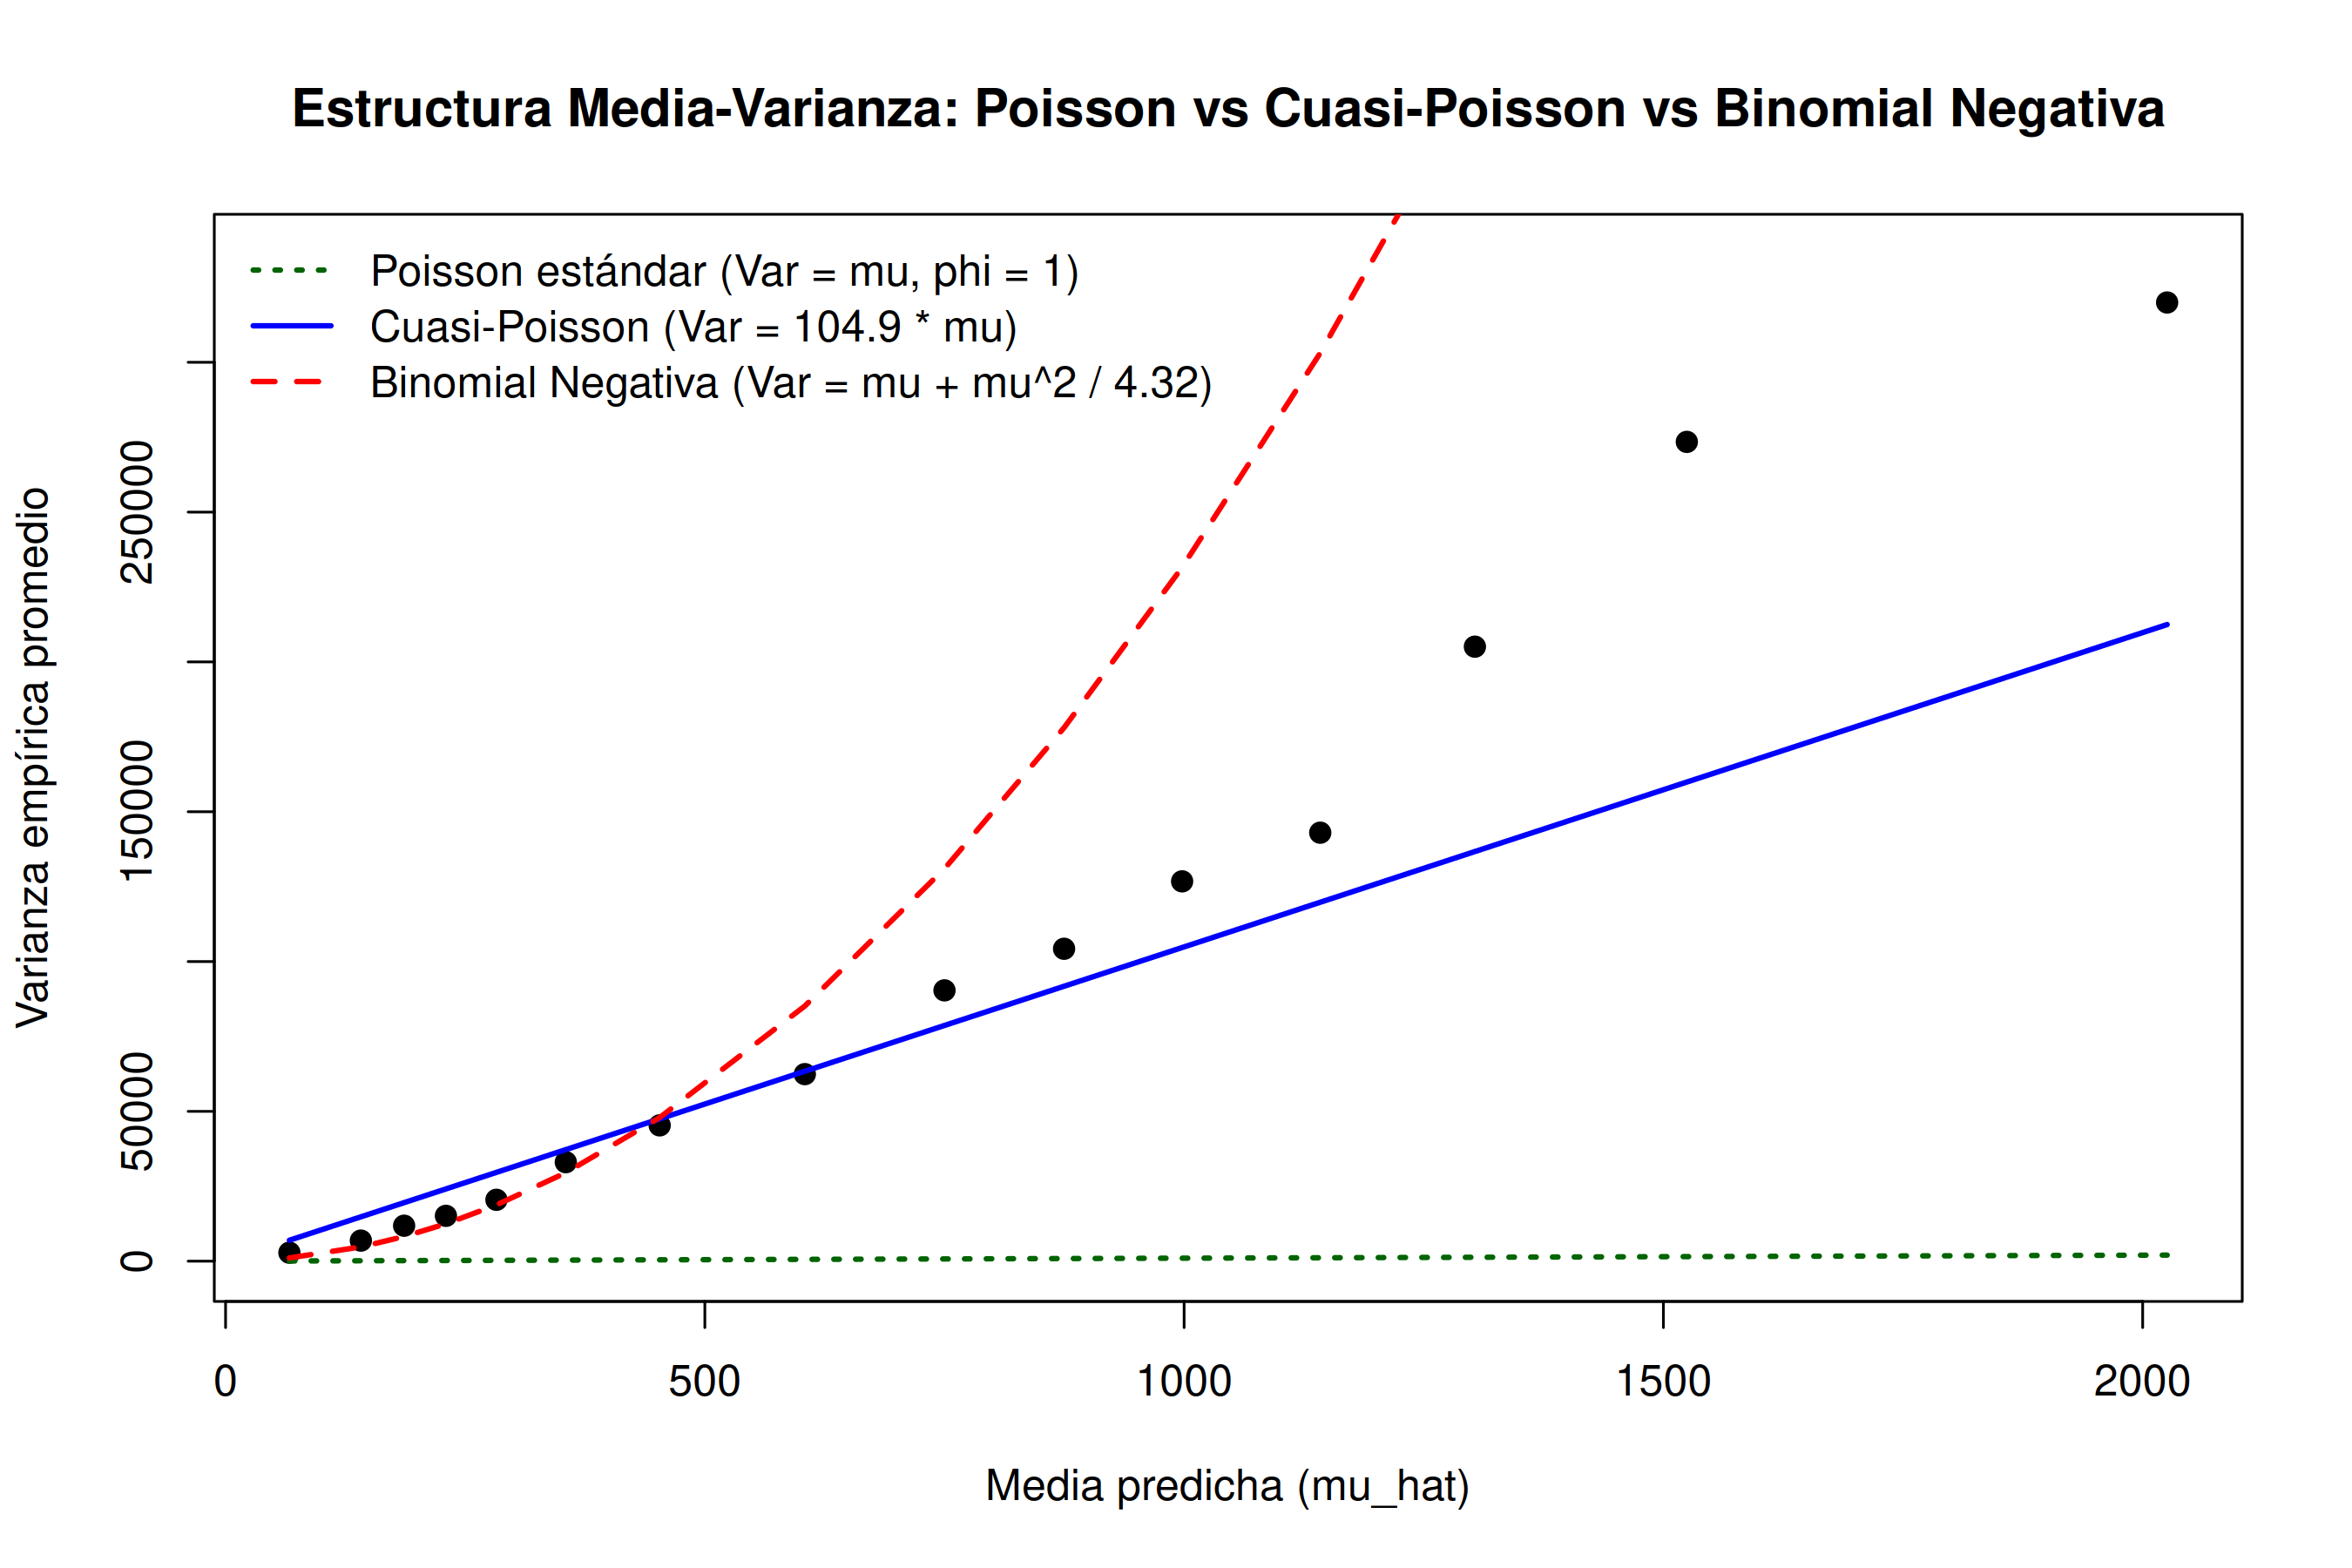
\includegraphics[width=0.82\textwidth]{plots/02_fit_media_varianza_modelo_base.png}
\caption{Relación media--varianza observada en 15 grupos y curvas teóricas de los modelos de conteo evaluados. Los grupos se forman con las medias ajustadas del modelo cuasi-Poisson aditivo sin visibilidad (modelo base). Las curvas usan $\widehat\phi\approx104{,}9$, estimado en el modelo cuasi-Poisson aditivo inicial (con visibilidad), y $\widehat\theta\approx4{,}32$, estimado en un modelo binomial negativo con ese mismo predictor inicial.}
\label{fig:varmedia}
\end{figure}

La estructura Poisson subestima considerablemente la variabilidad observada.
Si bien las estructuras cuasi-Poisson y binomial negativa representan mejor el comportamiento empírico, ninguna reproduce exactamente la variabilidad en todo el rango de medias. Se adopta cuasi-Poisson como modelo de trabajo por su estructura de momentos y porque conserva el predictor de media del Poisson.

\newpage

\subsection{Selección de modelos mediante pruebas $F$ y reducción de devianza}\label{sec:seleccion}
Para seleccionar los términos del predictor lineal se utilizaron dos criterios en conjunto: el valor-$p$ de una prueba $F$ y la reducción porcentual de devianza.

Sean $M_R\subset M_C$ dos modelos anidados, con devianzas residuales $D_R,D_C$ y número de parámetros estimables $p_R,p_C$. Se definen
\begin{equation}\label{eq:criterio}
\Delta D=D_R-D_C,\qquad R_D=100\frac{\Delta D}{D_R},\qquad q=p_C-p_R,
\end{equation}
donde $R_D$ es el porcentaje de reducción de devianza respecto al modelo reducido y $q$ el número de parámetros adicionales. Como el modelo cuasi-Poisson no tiene una verosimilitud completa, para comparar ambos modelos se utilizó la prueba $F$ \cite{mccullagh,dunn}
\[
F=\frac{\Delta D/q}{\widehat\phi_C}\sim F_{q,\,n-p_C},
\]
donde $\widehat\phi_C$ es la dispersión estimada del modelo completo.

\textbf{Depuración de efectos principales.} Se partió del modelo aditivo con las 11 covariables y se evaluó, mediante la prueba $F$, la eliminación de cada efecto principal manteniendo los restantes. La única variable no significativa al $5\%$ fue la visibilidad, cuya eliminación además prácticamente no modificó la devianza, por lo que se excluyó. El modelo resultante, con 10 covariables, se usó como modelo base.

\textbf{Preselección de interacciones.} Con las 10 covariables del modelo base se formaron las 45 interacciones de segundo orden posibles. Cada una se agregó por separado al modelo base y se consideró candidata si cumplía ambas condiciones:
\begin{enumerate}
\item valor-$p$ de la prueba $F$ menor que $0{,}05$;
\item reducción de devianza de al menos un $2\%$ ($R_D\geq 2$).
\end{enumerate}

\textbf{Selección iterativa de interacciones.} Con las candidatas se construyó el modelo de manera progresiva:
\begin{enumerate}
\item En cada paso, cada candidata aún no incluida se agregó por separado al modelo actual y se calcularon su valor-$p$ y su $R_D$ respecto de dicho modelo.
\item Se conservaron solo las candidatas que cumplían ambas condiciones: valor-$p<0{,}05$ y $R_D\geq 2$.
\item Estas candidatas se ordenaron de menor a mayor valor-$p$ y se incorporó al modelo la de menor valor-$p$.
\item Con el modelo actualizado se repitió el procedimiento con las candidatas restantes. El proceso terminó cuando ninguna de ellas cumplía ambas condiciones.
\end{enumerate}
Al incorporar una interacción se mantuvieron siempre los efectos principales de las variables involucradas.

\textbf{Limitaciones del criterio basado en valores-$p$.} La prueba $F$ supone observaciones independientes. Durante la selección se observó que prácticamente todas las comparaciones entregaban valores-$p$ extremadamente pequeños, muchos de ellos prácticamente cero, incluso para términos con aportes modestos a la devianza. Esto hizo sospechar que el supuesto de independencia no se cumplía, lo que se confirmó posteriormente en el diagnóstico de residuos, donde la autocorrelación muestra una dependencia temporal marcada entre registros horarios. Con observaciones dependientes, las pruebas $F$ tienden a declarar significativos términos que no necesariamente lo son. Por esta razón, los valores-$p$ se utilizaron solo como una regla para ordenar y filtrar términos, y no como evidencia inferencial formal. Por el mismo motivo se exigió además una reducción mínima de devianza del $2\%$, de modo que solo se incorporaran términos con relevancia práctica. Finalmente, la capacidad de generalización del modelo se evaluó mediante validación cruzada por bloques de días completos.
\newpage

\subsection{Diagnóstico del ajuste y validación predictiva}
Para evaluar el cumplimiento de los supuestos estructurales del modelo seleccionado y verificar su capacidad de generalización fuera de muestra, se emplearon las siguientes herramientas \cite{dunn}:

\begin{itemize}
    \item \textbf{Análisis de residuos y linealidad:} Se calcularon los residuos de devianza estandarizados,
    \[
    r_i^* = \frac{\operatorname{sign}(y_i - \widehat{\mu}_i)\sqrt{d_i}}{\sqrt{\widehat{\phi}(1 - h_{ii})}},
    \]
    donde $d_i = 2\left[y_i\log(y_i/\widehat{\mu}_i) - (y_i - \widehat{\mu}_i)\right]$ corresponde a la devianza individual y $h_{ii}$ es el elemento diagonal de la matriz sombrero generalizada, definida por:
    \begin{align*}
    \widehat{\mathbf{H}} &= \widehat{\mathbf{W}}^{1/2}\mathbf{X}(\mathbf{X}^{\mathsf T}\widehat{\mathbf{W}}\mathbf{X})^{-1}\\
    &\qquad\cdot \mathbf{X}^{\mathsf T}\widehat{\mathbf{W}}^{1/2}.
    \end{align*}
    Estos residuos se graficaron frente al predictor lineal $\widehat{\eta}_i$ y frente a la temperatura $T_i$, superponiendo curvas suavizadas \textit{LOWESS} para detectar posibles desviaciones sistemáticas o curvaturas no lineales remanentes.

    \item \textbf{Observaciones influyentes y análisis de sensibilidad:} Se identificaron registros atípicos mediante el umbral $|r_i^*| > 3$, puntos de alto apalancamiento mediante $h_{ii} > 2p/n$ y observaciones influyentes mediante la distancia de Cook aproximada para modelos lineales generalizados \cite{dunn},
    \[
    D_i = \frac{r_{P,i}^2}{p\,\widehat{\phi}}\left(\frac{h_{ii}}{(1 - h_{ii})^2}\right),
    \]
    utilizando como referencia el corte $D_i > 4/n$, donde $r_{P,i} = (y_i - \widehat{\mu}_i)/\sqrt{\widehat{\mu}_i}$ es el residuo de Pearson. Para evaluar la estabilidad del ajuste, se reestimó el modelo excluyendo las 10 observaciones con mayor distancia de Cook y se comparó la variación en los coeficientes estimados y en el parámetro de dispersión $\widehat{\phi}$ para ver qué tanto efecto tenían esas observaciones.

    \item \textbf{Autocorrelación temporal:} Dada la naturaleza horaria consecutiva de los registros, se inspeccionó la función de autocorrelación muestral (ACF) de los residuos de Pearson hasta el rezago $k = 39$ (valor por defecto de \texttt{acf} en \texttt{R}) para evaluar el supuesto de independencia condicional entre observaciones.

    \item \textbf{Métricas de validación cruzada:} Sobre los $K = 10$ pliegues agrupados por días completos \cite{roberts}, se cuantificó el desempeño predictivo en la escala original de conteos mediante la raíz del error cuadrático medio ($\text{RMSE}$) y el error absoluto medio ($\text{MAE}$):
    \[
    \text{RMSE} = \sqrt{\frac{1}{n}\sum_{i=1}^n (y_i - \widehat{\mu}_i)^2}, \qquad
    \text{MAE} = \frac{1}{n}\sum_{i=1}^n |y_i - \widehat{\mu}_i|,
    \]
    comparando los errores dentro de muestra (\textit{Train}) frente a los errores fuera de muestra (\textit{CV}) para descartar sobreajuste.
\end{itemize}
\FloatBarrier
\section{Resultados}

\subsection{Depuración de los efectos principales}

A partir del modelo aditivo completo, constituido por
11 covariables y 41 parámetros estimables, se evaluó
el aporte individual de cada covariable al ajuste
mediante su eliminación del predictor lineal,
manteniendo los restantes efectos principales.

En particular, al retirar la visibilidad del modelo,
se obtuvo un incremento aproximado de devianza de

\[
\Delta D \approx 1{,}47,
\]

lo que representa un incremento porcentual de
aproximadamente $0{,}00016\%$ respecto de la devianza
del modelo aditivo completo.

\begin{table}[htbp]
\centering
\caption{Comparación de los modelos aditivos con y
sin visibilidad.}
\label{tab:depuracion}
\begin{adjustbox}{max width=\linewidth}
\begin{tabular}{lrrr}
\toprule
Modelo & Covariables & Parámetros & Devianza \\
\midrule
Aditivo completo
& 11 & 41 & 904\,697 \\
Aditivo sin visibilidad
& 10 & 40 & 904\,698 \\
\bottomrule
\end{tabular}
\end{adjustbox}
\end{table}

Como se observa en la Tabla \ref{tab:depuracion},
la eliminación de la visibilidad no produce un
deterioro considerable en el ajuste. Por consiguiente,
siguiendo el principio de parsimonia, se decidió
excluir esta variable, puesto que permite reducir
la complejidad del modelo conservando prácticamente
la misma devianza residual.

Respecto de las variables excluidas durante el
preprocesamiento, la temperatura de punto de rocío
presentó una correlación de Pearson de $0{,}91$ con
la temperatura, por lo que se decidió conservar
únicamente esta última.

Por otra parte, se excluyeron las 295 observaciones
correspondientes a horas en las que el servicio no
se encontraba operativo, equivalentes al $3{,}37\%$
de las 8\,760 observaciones originales. De esta
manera, la variable de funcionamiento del servicio
dejó de presentar variabilidad en la muestra efectiva.

En cuanto a las precipitaciones, se registraron
516 horas con lluvia ($6{,}10\%$) y 443 horas con
nieve ($5{,}23\%$), sobre un total de 8\,465
observaciones. Debido a la elevada proporción de
registros sin precipitaciones, se utilizaron
variables indicadoras de presencia o ausencia,
en lugar de sus respectivas intensidades.
Además, en un primer ajuste del modelo aditivo
con la lluvia y la nieve como variables continuas
(en mm y cm), la dispersión estimada resultó
enorme, $\widehat\phi\approx1{,}5\times10^{6}$,
frente a $\widehat\phi\approx104{,}9$ al
utilizar las variables indicadoras, y la devianza
residual también fue mayor ($974\,882$ frente a
$904\,697$). Por este motivo, y por simplicidad
en la interpretación, se optó por mantener ambas
variables en forma binaria.
\newpage

Finalmente, los valores del factor de inflación
de la varianza generalizado ajustado \cite{fox} satisficieron

\[
\mathrm{GVIF}^{1/(2\,\mathrm{gl})}<2{,}4,
\]

por lo que no se encontraron indicios de
multicolinealidad severa que justificaran la
exclusión de otras covariables.

El modelo aditivo reducido quedó constituido por
diez covariables: hora del día, temperatura,
humedad, velocidad del viento, radiación solar,
estación del año, día feriado, lluvia, nieve
y día de la semana.

Este modelo contiene 40 parámetros estimables,
presenta una devianza residual de $904\,698$
y explica el $80{,}14\%$ de la devianza del modelo
nulo.
Sobre este modelo se realizó la posterior
incorporación de interacciones.
\subsection{Selección de interacciones}

De las 45 interacciones evaluadas individualmente respecto del modelo base, el procedimiento implementado preseleccionó diez. La Tabla~\ref{tab:res_candidatas} presenta sus reducciones de devianza y el número de parámetros adicionales. La última columna permite comparar descriptivamente el aporte de cada interacción en relación con su complejidad.

\begin{table}[htbp]
\centering\small
\caption{Aporte individual de las interacciones preseleccionadas respecto del modelo base.}
\label{tab:res_candidatas}
\begin{adjustbox}{max width=\linewidth}
\begin{tabular}{lrrr}\toprule
Interacción & $q$ & $R_D$ (\%) & $R_D/q$ \\\midrule
Temperatura $\times$ Radiación & 1 & 8{,}09 & 8{,}090 \\
Temperatura $\times$ Estación & 3 & 20{,}97 & 6{,}990 \\
Radiación $\times$ Estación & 3 & 7{,}22 & 2{,}407 \\
Humedad $\times$ Lluvia & 1 & 2{,}01 & 2{,}010 \\
Humedad $\times$ Estación & 3 & 3{,}58 & 1{,}193 \\
Hora $\times$ Temperatura & 23 & 8{,}80 & 0{,}383 \\
Radiación $\times$ Día de la semana & 6 & 2{,}22 & 0{,}370 \\
Hora $\times$ Radiación & 14 & 2{,}85 & 0{,}204 \\
Hora $\times$ Estación & 69 & 9{,}53 & 0{,}138 \\
Hora $\times$ Día de la semana & 138 & 18{,}44 & 0{,}134 \\\bottomrule
\end{tabular}
\end{adjustbox}
\end{table}

Las interacciones temperatura--radiación y temperatura--estación destacan por su reducción de devianza por parámetro adicional. En cambio, hora--día de la semana logra una reducción total del $18{,}44\%$, pero requiere 138 parámetros adicionales, lo que evidencia un mayor costo en complejidad.

La Tabla~\ref{tab:res_pasos} presenta la secuencia de incorporación obtenida en la selección iterativa. En cada paso se muestra la interacción elegida, es decir, la de menor valor-$p$ entre las que cumplían ambas condiciones, junto con su reducción de devianza respecto del modelo del paso anterior. Como los valores-$p$ son extremadamente pequeños, se reportan en escala $\log_{10}$.

\begin{table}[htbp]
\centering\small
\caption{Secuencia de incorporación de interacciones. Las reducciones y los valores-$p$ se refieren al modelo del paso anterior.}
\label{tab:res_pasos}
\begin{adjustbox}{max width=\linewidth}
\begin{tabular}{rlrrrr}\toprule
Paso & Interacción & $q$ & $R_D$ (\%) & $\log_{10}(\text{valor-}p)$ & Parámetros \\\midrule
0 & Base & -- & -- & -- & 40 \\
1 & Temperatura $\times$ Estación & 3 & 20{,}97 & $-433{,}9$ & 43 \\
2 & Hora $\times$ Día de la semana & 138 & 24{,}11 & $-401{,}7$ & 181 \\
3 & Hora $\times$ Temperatura & 23 & 12{,}51 & $-226{,}9$ & 204 \\
4 & Humedad $\times$ Lluvia & 1 & 4{,}21 & $-83{,}3$ & 205 \\
5 & Hora $\times$ Estación & 69 & 2{,}35 & $-15{,}1$ & 274 \\\bottomrule
\end{tabular}
\end{adjustbox}
\end{table}

La incorporación de términos se detuvo después de cinco interacciones. La Tabla~\ref{tab:res_restantes} muestra las cinco candidatas que no fueron incorporadas, evaluadas respecto del modelo final. Todas siguen siendo significativas al $5\%$, pero ninguna alcanza una reducción de devianza del $2\%$, por lo que ninguna cumple ambas condiciones.

\begin{table}[htbp]
\centering\small
\caption{Candidatas no incorporadas, evaluadas respecto del modelo final.}
\label{tab:res_restantes}
\begin{adjustbox}{max width=\linewidth}
\begin{tabular}{lrrr}\toprule
Interacción & $q$ & $R_D$ (\%) & $\log_{10}(\text{valor-}p)$ \\\midrule
Hora $\times$ Radiación & 14 & 1{,}70 & $-24{,}2$ \\
Temperatura $\times$ Radiación & 1 & 1{,}20 & $-24{,}1$ \\
Radiación $\times$ Estación & 3 & 0{,}57 & $-10{,}1$ \\
Radiación $\times$ Día de la semana & 6 & 0{,}54 & $-7{,}8$ \\
Humedad $\times$ Estación & 3 & 0{,}26 & $-4{,}3$ \\\bottomrule
\end{tabular}
\end{adjustbox}
\end{table}

En particular, temperatura--radiación pasó de aportar un $8{,}09\%$ individualmente a un $1{,}20\%$ respecto del modelo final, lo que sugiere que parte de su aporte ya estaba recogido por los términos incorporados. Que todas las candidatas restantes sigan siendo significativas confirma que, con estos datos, el valor-$p$ por sí solo no permite detener la selección, y que el criterio de reducción mínima de devianza es el que determina el tamaño del modelo.

Desde el punto de vista de la parsimonia, temperatura--estación y humedad--lluvia proporcionan mejoras relativamente grandes con pocos parámetros. Por el contrario, hora--estación aporta una reducción del $2{,}35\%$ con 69 parámetros adicionales. En consecuencia, el modelo obtenido mejora el ajuste, pero no se puede afirmar que sea el más parsimonioso.

\newpage

\subsection{Modelo seleccionado e interpretación}

Sea $\eta_i^{(B)}$ el predictor del modelo base, es decir, el predictor lineal inicial definido en la Sección de metodología sin el término de visibilidad $\beta_4A_i$. El modelo final contiene 274 coeficientes estimables y, respecto de $\eta_i^{(B)}$, incorpora las siguientes interacciones:
\begin{align*}
\eta_i^{(F)}={}&\eta_i^{(B)}
+\sum_{j\in\{P,V,I\}} a_j T_i\mathbb{I}(E_i=j)\\
&+\sum_{h=1}^{23}\sum_{d=1}^{6} b_{hd}\mathbb{I}(H_i=h)\mathbb{I}(W_i=d)\\
&+\sum_{h=1}^{23} c_h T_i\mathbb{I}(H_i=h)+\xi U_iL_i\\
&+\sum_{h=1}^{23}\sum_{j\in\{P,V,I\}} e_{hj}\mathbb{I}(H_i=h)\mathbb{I}(E_i=j),
\end{align*}
donde se utilizan las categorías de referencia del modelo base. Las medias ajustadas son $\widehat\mu_i=\exp(\widehat\eta_i^{(F)})$.

\paragraph{Temperatura.} Debido a sus interacciones con la estación y la hora, la razón de medias estimadas asociada a un aumento de $1\,^{\circ}$C, para una estación $j$ y una hora $h$, es
\[
\exp(\widehat\beta_T+\widehat a_j+\widehat c_h),
\]
con los coeficientes de interacción iguales a cero en sus respectivas categorías de referencia. Por tanto, no existe una única razón de medias para todas las estaciones y horas.

\paragraph{Hora del día.} Las interacciones hora--día de la semana y hora--estación permiten representar perfiles horarios diferentes según el día y la estación, en lugar de imponer una misma forma del perfil diario.

\paragraph{Lluvia y humedad.} Para una humedad relativa $u$, la razón de medias estimadas entre presencia y ausencia de lluvia, manteniendo las demás variables constantes, es
\[
\exp(\widehat\lambda+\widehat\xi u),
\]
donde $\widehat\lambda\approx1{,}99$ es el coeficiente principal de lluvia estimado en el modelo final.
Su interpretación aislada corresponde a humedad cero y no representa la asociación general de la lluvia con la demanda.

\subsection{Evaluación descriptiva del ajuste}

\begin{table}[htbp]
\centering\small
\caption{Comparación descriptiva de los modelos cuasi-Poisson.}
\label{tab:res_ajuste}
\begin{adjustbox}{max width=\linewidth}
\begin{tabular}{lrrrrr}\toprule
Modelo & $p$ & gl resid. & $D$ & Dev. exp. (\%) & $\widehat\phi$ \\\midrule
Nulo & 1 & 8464 & $4\,556\,385$ & 0{,}00 & 565{,}88 \\
Base & 40 & 8425 & $904\,698$ & 80{,}14 & 104{,}89 \\
Final & 274 & 8191 & $444\,099$ & 90{,}25 & 50{,}89 \\\bottomrule
\end{tabular}
\end{adjustbox}
\end{table}

La Tabla~\ref{tab:res_ajuste} muestra que la incorporación de interacciones reduce la devianza residual del modelo base en un $50{,}91\%$ y aumenta el porcentaje de devianza explicada de $80{,}14\%$ a $90{,}25\%$. Esta mejora se obtiene a costa de 234 parámetros adicionales. Asimismo, la dispersión estimada disminuye de $104{,}89$ a $50{,}89$, aunque sigue siendo considerablemente mayor que uno. Por tanto, el modelo final representa mejor la demanda observada, pero conserva una variabilidad residual elevada y un costo importante en complejidad.

\subsection{Diagnóstico del ajuste y limitaciones de la inferencia}

La Figura~\ref{fig:diag_fwd} resume el diagnóstico del modelo final: (A) residuos de devianza estandarizados frente al predictor lineal, (B) residuos frente a la temperatura, (C) distancia de Cook y (D) función de autocorrelación de los residuos de Pearson.

\begin{figure}[htbp]
\centering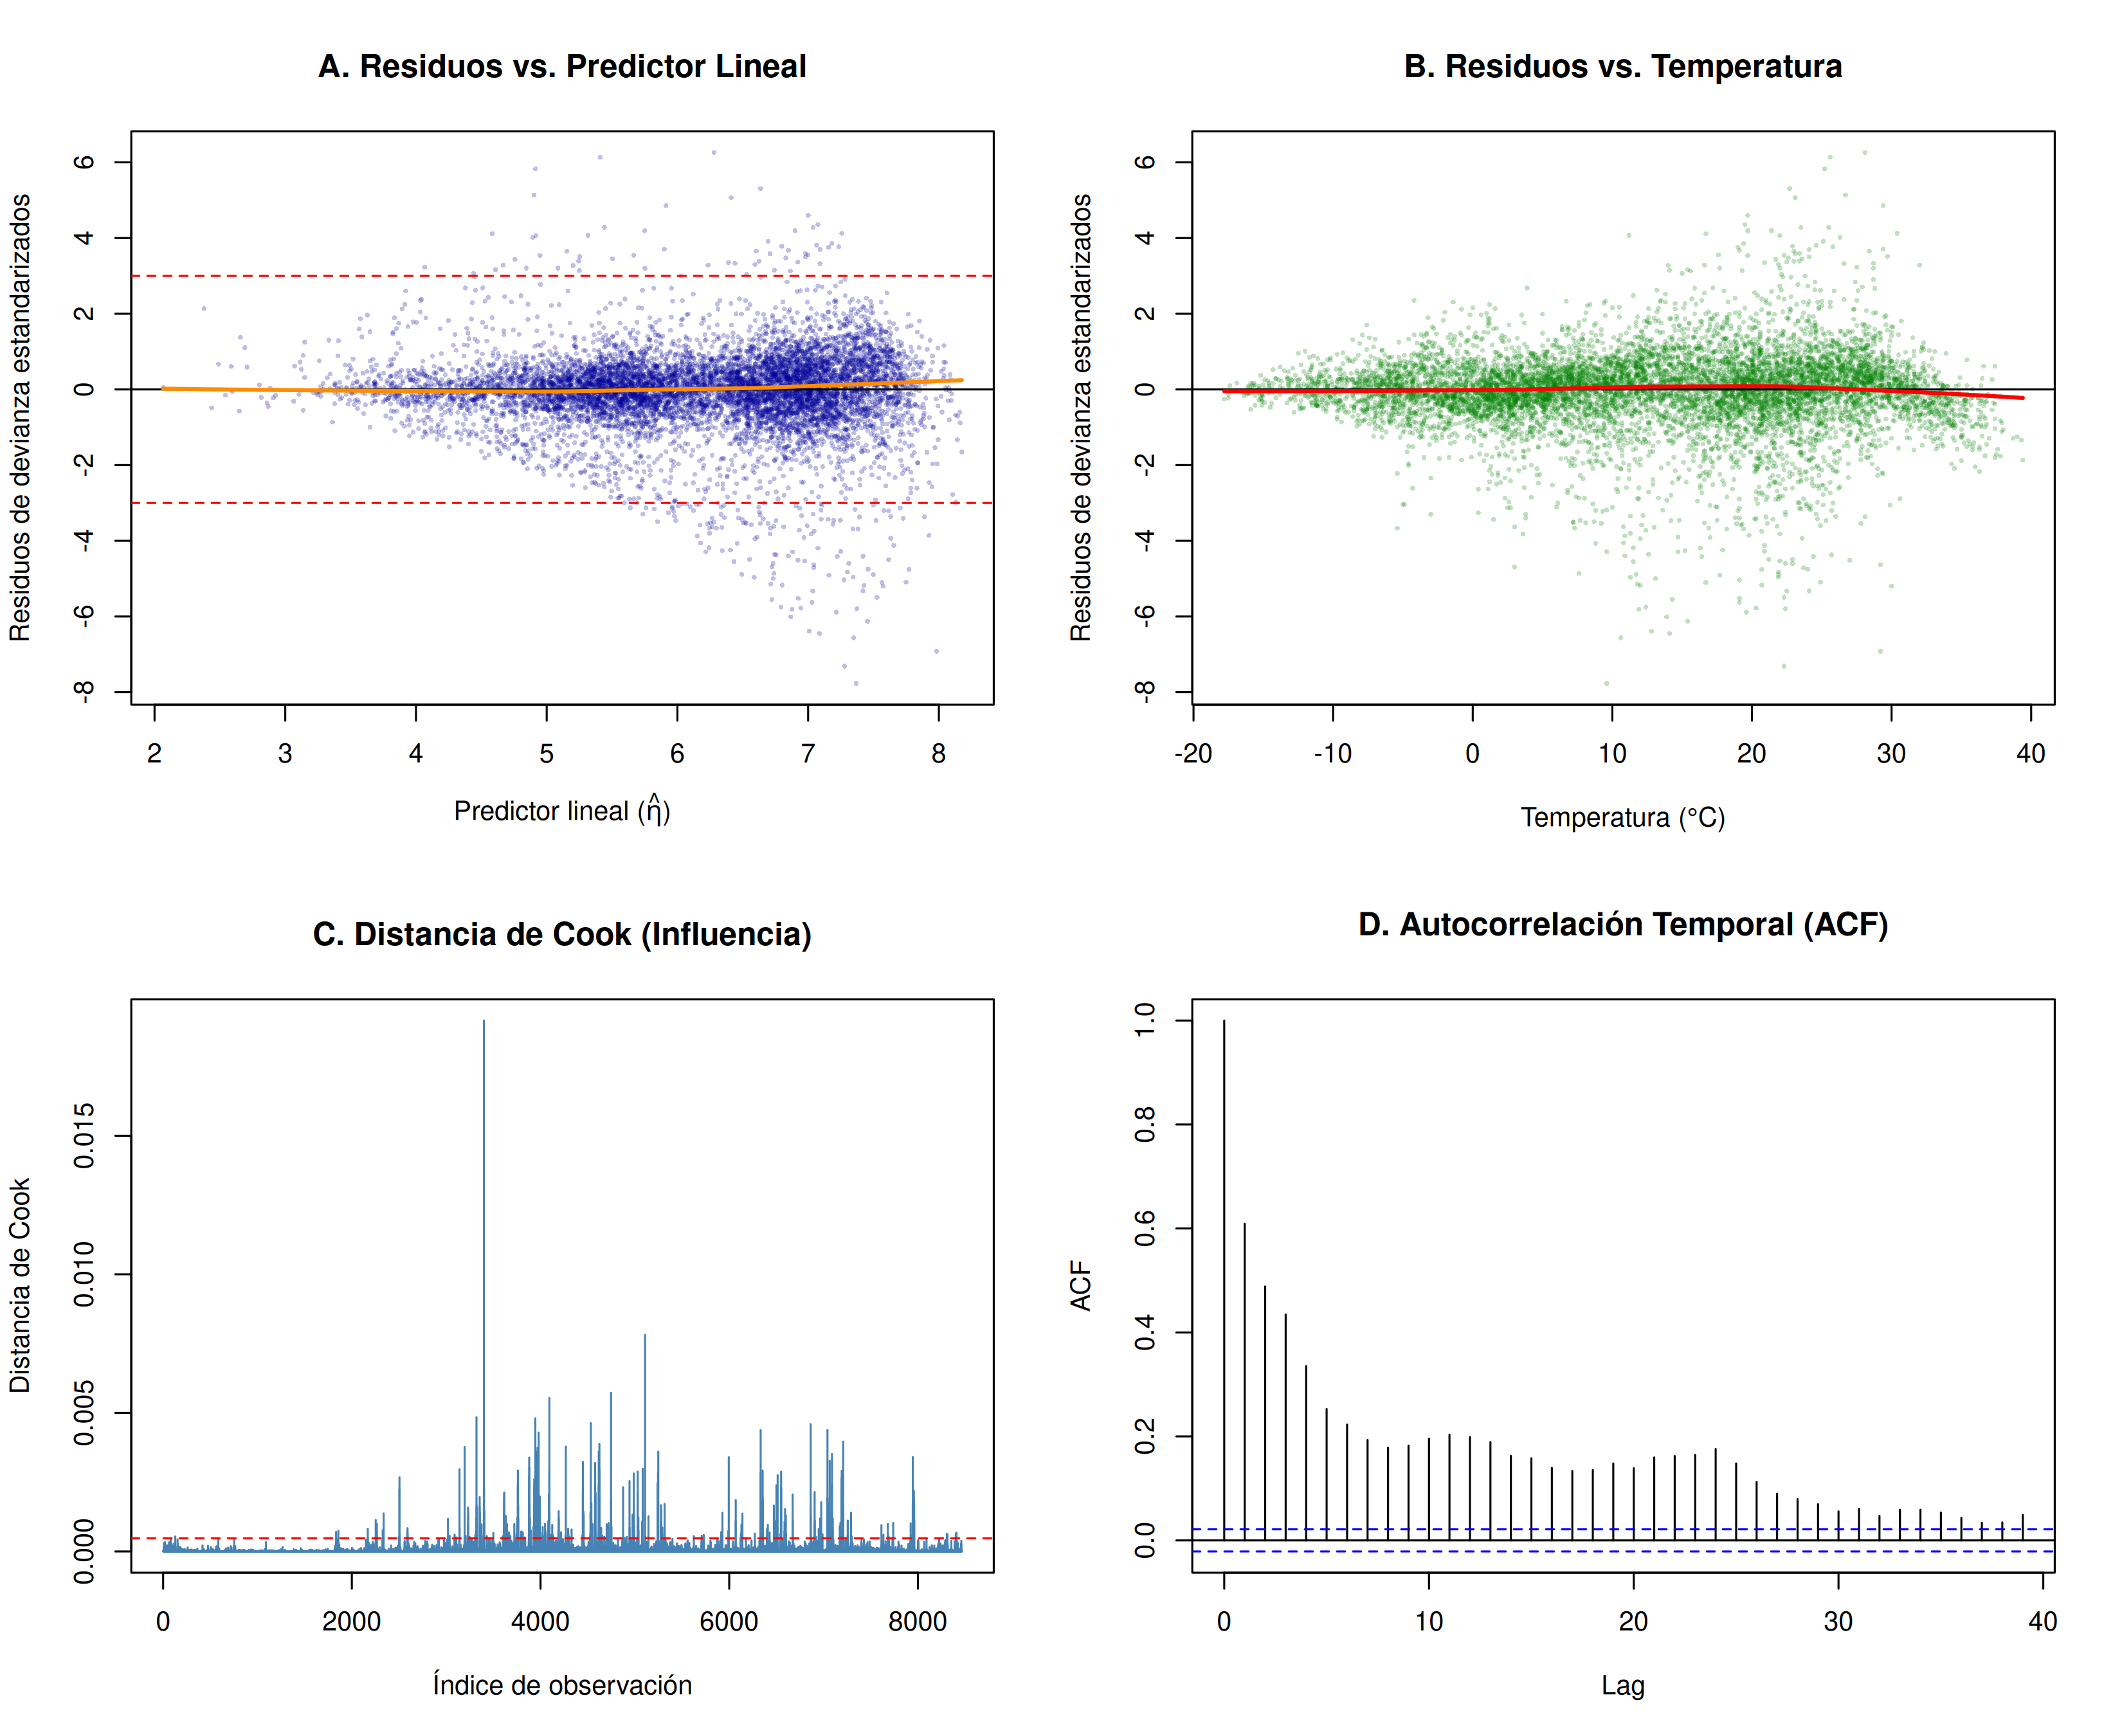
\includegraphics[width=.95\textwidth]{plots/02_fit_diagnostico_residuos_m_fwd.png}
\caption{Diagnóstico de residuos y observaciones influyentes del modelo final.}
\label{fig:diag_fwd}
\end{figure}

\paragraph{Residuos.} De las $8\,465$ observaciones, 483 ($5{,}7\%$) tienen residuos de devianza estandarizados mayores que 2 en valor absoluto y 204 ($2{,}4\%$) mayores que 3. La curva suavizada (LOWESS) de los residuos frente al predictor lineal se mantiene entre $-0{,}05$ y $0{,}24$, y frente a la temperatura entre $-0{,}23$ y $0{,}09$, por lo que no se observa una curvatura marcada en ninguno de los dos casos.

Como en el panel A la mayoría de los puntos se concentra en valores altos del predictor lineal, se agruparon los residuos en 30 intervalos con igual número de observaciones (Figura~\ref{fig:res_bin}). Los promedios por intervalo varían entre $-0{,}26$ y $0{,}16$ y, en general, son levemente negativos. En 9 de los 30 intervalos el promedio se aleja de cero en más de dos errores estándar. Las mayores desviaciones se encuentran en los extremos: el intervalo de menor demanda predicha tiene un promedio de $0{,}14$ y el de mayor demanda predicha uno de $-0{,}26$. Esto indica que el modelo tiende a subestimar levemente las demandas más bajas y a sobreestimar las más altas, aunque las desviaciones son pequeñas en comparación con la escala de los residuos.

\begin{figure}[htbp]
\centering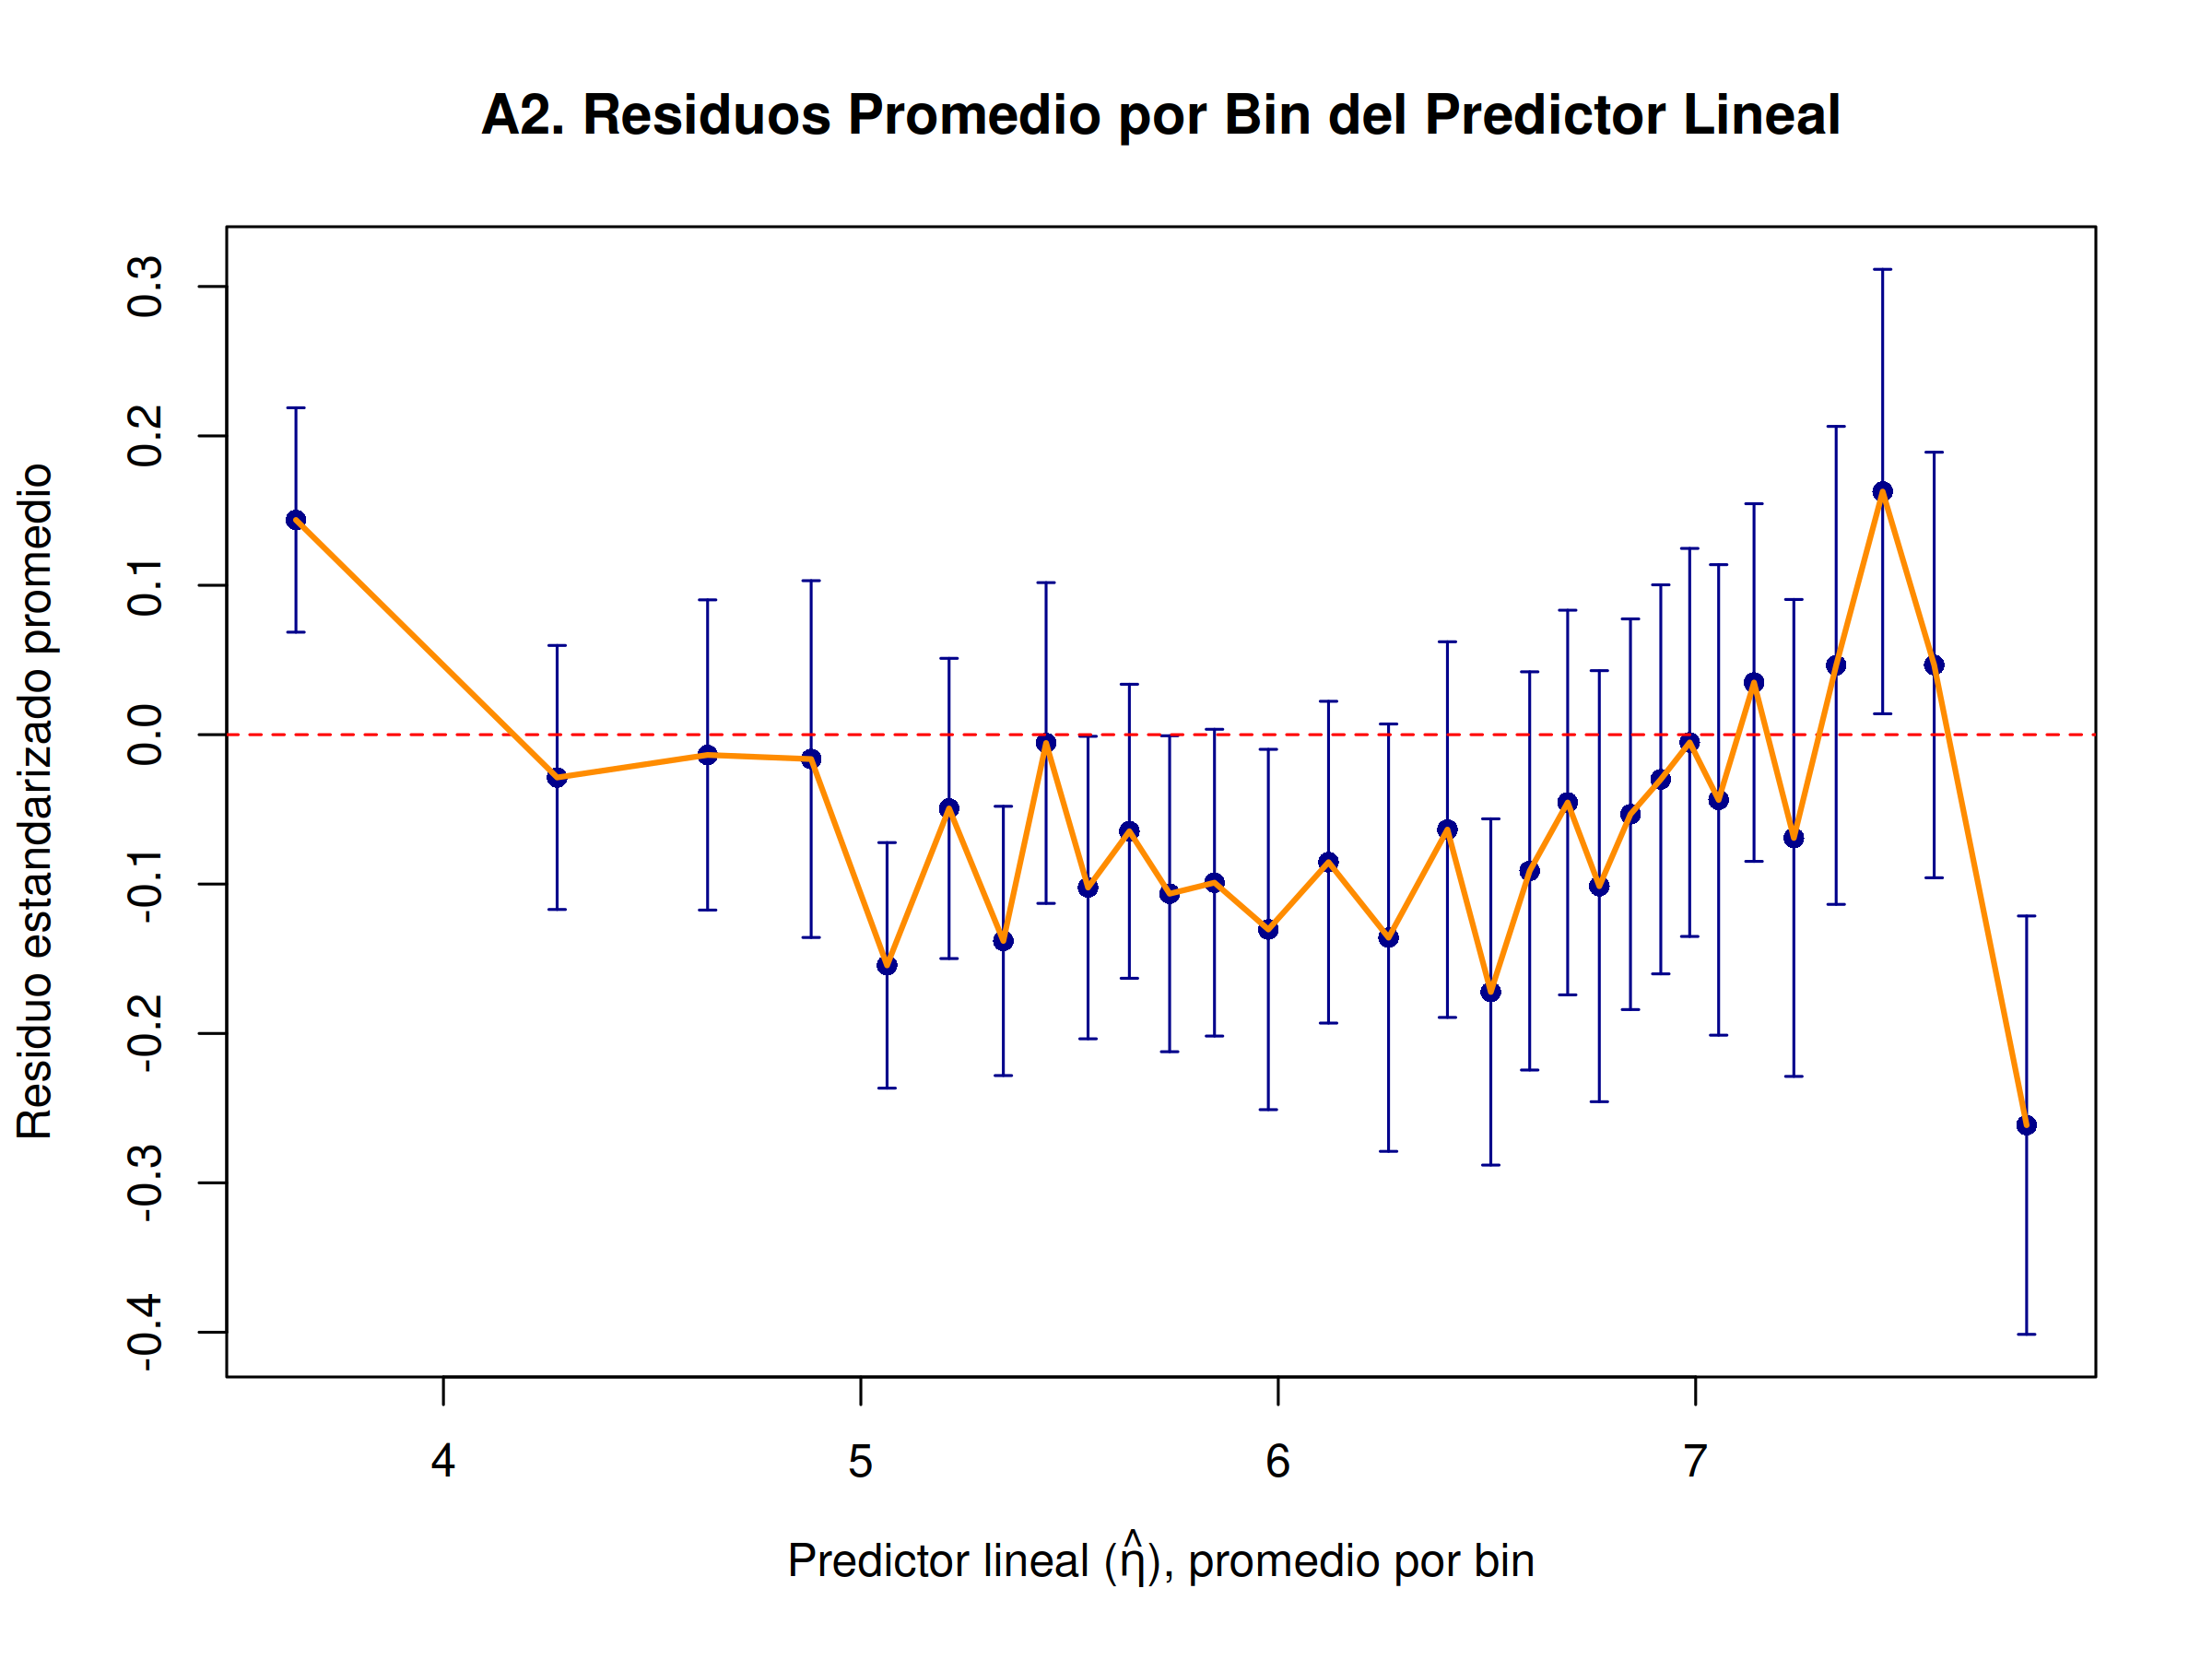
\includegraphics[width=.75\textwidth]{plots/02_fit_residuos_por_bin_m_fwd.png}
\caption{Promedio de los residuos de devianza estandarizados en 30 intervalos del predictor lineal, con bandas de $\pm2$ errores estándar.}
\label{fig:res_bin}
\end{figure}

\paragraph{Observaciones influyentes.} La distancia de Cook máxima es $0{,}019$, muy inferior a 1, aunque 432 observaciones superan el umbral orientativo $4/n$. La observación más influyente corresponde al 22 de abril de 2018 a las 15:00, una hora con lluvia en la que se registraron 234 arriendos frente a 1362 ajustados. Entre las diez observaciones con mayor distancia de Cook, cuatro corresponden a horas con lluvia, aunque solo 516 de las $8\,465$ horas de la muestra presentan lluvia. En este grupo también aparece el residuo más extremo, el del 19 de abril de 2018 a las 08:00, con 20 arriendos observados frente a 1582 ajustados.

\begin{table}[htbp]
\centering\small
\caption{Sensibilidad de los coeficientes al excluir las diez observaciones con mayor distancia de Cook.}
\label{tab:res_sens}
\begin{adjustbox}{max width=\linewidth}
\begin{tabular}{lrr}\toprule
Coeficiente & Diferencia absoluta & Cambio multiplicativo (\%) \\\midrule
Lluvia (sí) & 0{,}472 & 60{,}3 \\
Hora 13 $\times$ Martes & 0{,}038 & 3{,}9 \\
Hora 8 $\times$ Verano & 0{,}032 & 3{,}3 \\
Hora 22 $\times$ Verano & 0{,}031 & 3{,}1 \\
Hora 18 $\times$ Miércoles & 0{,}028 & 2{,}8 \\\bottomrule
\end{tabular}
\end{adjustbox}
\end{table}

Al reajustar el modelo sin estas diez observaciones, la mayor variación corresponde al coeficiente principal de lluvia (Tabla~\ref{tab:res_sens}), que pasa de $1{,}99$ a $2{,}46$. El resto de los coeficientes cambia menos de un $4\%$ en escala multiplicativa. La dispersión disminuye de $50{,}89$ a $49{,}31$. Estos resultados aconsejan cautela al interpretar los términos relacionados con la lluvia, pero no justifican eliminar estas observaciones, que corresponden a registros reales.

\paragraph{Autocorrelación.} La autocorrelación de los residuos de Pearson es $0{,}61$ en el primer rezago, $0{,}49$ en el segundo y $0{,}18$ en el rezago 24. Debido a la exclusión de horas sin funcionamiento, los rezagos se refieren a registros disponibles y no necesariamente a horas consecutivas de reloj. Esta dependencia confirma la sospecha planteada durante la selección del modelo (Sección~\ref{sec:seleccion}): las observaciones no son independientes, por lo que los errores estándar y los valores-$p$ del cuasi-Poisson son demasiado optimistas. Por ello, las pruebas $F$ se utilizaron solo como regla de selección y las comparaciones de ajuste se interpretan de forma descriptiva.

\subsection{Validación descriptiva por bloques temporales}

\begin{table}[htbp]
\centering\small
\caption{Errores de entrenamiento y validación cruzada por días completos (semilla 123).}
\label{tab:res_cv}
\begin{adjustbox}{max width=\linewidth}
\begin{tabular}{lrrrr}\toprule
Modelo & RMSE Train & RMSE CV & MAE Train & MAE CV \\\midrule
Base & 312{,}08 & 318{,}41 & 207{,}25 & 212{,}42 \\
Final & 206{,}00 & 215{,}96 & 125{,}05 & 131{,}55 \\\bottomrule
\end{tabular}
\end{adjustbox}
\end{table}

El modelo final reduce el RMSE de validación en aproximadamente un $32{,}2\%$ y el MAE en un $38{,}1\%$ respecto del modelo base. Si bien la brecha relativa entre entrenamiento y validación aumenta hasta el $4{,}8\%$ para RMSE y el $5{,}2\%$ para MAE, los errores de validación son considerablemente menores. Estas brechas corresponden a la semilla 123; al usar el promedio de los errores de validación de las cinco semillas (Tabla~\ref{tab:conclusion_cv}) resultan de $5{,}0\%$ y $5{,}3\%$, respectivamente.

\begin{table}[htbp]
\centering\small
\caption{Promedio y desviación estándar de los errores de validación para cinco semillas.}
\label{tab:res_semillas}
\begin{adjustbox}{max width=\linewidth}
\begin{tabular}{lrr}\toprule
Modelo & RMSE CV & MAE CV \\\midrule
Base & $318{,}99\pm1{,}35$ & $212{,}37\pm0{,}78$ \\
Final & $216{,}25\pm0{,}96$ & $131{,}66\pm0{,}36$ \\\bottomrule
\end{tabular}
\end{adjustbox}
\end{table}

La mejora se mantiene en las cinco particiones estudiadas. Sin embargo, los días fueron asignados aleatoriamente a los pliegues y la selección de interacciones se realizó previamente con la muestra completa. Por ello, la validación respalda descriptivamente la capacidad predictiva de la fórmula ajustada, pero no garantiza la ausencia de sobreajuste ni equivale a una evaluación de pronósticos futuros.$\\$ 
\newpage

\section{Conclusiones}

\subsection{Respuesta a las preguntas de investigación}

\textbf{Pregunta principal:}
¿Cómo se relacionan las condiciones climáticas y temporales
con la cantidad de bicicletas arrendadas por hora en la
ciudad de Seúl?

Los resultados obtenidos muestran que las condiciones
climáticas y temporales permiten explicar una parte
importante del comportamiento de la demanda horaria de
bicicletas. En particular, la hora del día, la temperatura,
la estación del año y la presencia de lluvia son variables
que presentan aportes importantes al ajuste del modelo.

En contraste, la exclusión de la visibilidad genera un
incremento de devianza de aproximadamente $0{,}00016\%$,
por lo que se decidió prescindir de esta variable,
considerando el principio de parsimonia.

El modelo aditivo explica el $80{,}14\%$ de la devianza
del modelo nulo, mientras que la incorporación de
interacciones permite aumentar este porcentaje al
$90{,}25\%$, reduciendo la devianza residual en un
$50{,}91\%$ respecto del modelo aditivo.

Esto indica que considerar únicamente los efectos
principales no permite representar completamente las
relaciones presentes en los datos. En particular,
las interacciones permiten que la asociación de una
covariable con la demanda dependa de los valores
o categorías de otras covariables.

Sin embargo, esta mejora implica aumentar el número
de parámetros estimables de 40 a 274, lo que evidencia
un compromiso entre la calidad del ajuste y la
parsimonia del modelo.

Respecto de la capacidad predictiva, el modelo final
presentó un RMSE promedio de validación cruzada de
$216{,}25$ y un MAE de $131{,}66$ bicicletas por hora,
frente a los valores de $318{,}99$ y $212{,}37$,
respectivamente, obtenidos con el modelo aditivo.

Por consiguiente, bajo la especificación considerada,
la incorporación de interacciones permite representar
de mejor manera la demanda observada y obtener menores
errores de predicción en las particiones evaluadas.

\paragraph{Por qué la evaluación se basa en validación cruzada.}
Como se mostró en el diagnóstico, los residuos del modelo presentan una autocorrelación marcada ($0{,}61$ en el primer rezago). Por ello, los valores-$p$ de las pruebas $F$, que resultaron extremadamente pequeños para casi todos los términos, no son confiables como evidencia inferencial: suponen observaciones independientes y, al no cumplirse este supuesto, tienden a declarar significativos incluso términos con aportes muy pequeños (entre los efectos principales, solo la visibilidad resultó no significativa). En consecuencia, las conclusiones sobre la relación entre las variables y la demanda no se basan en la significancia de los coeficientes, sino en la capacidad del modelo para predecir datos que no utilizó en su ajuste y en la magnitud de los efectos que estima.

Para ello se aplicó validación cruzada por bloques de 10 pliegues, donde cada bloque corresponde a días completos, de modo que las 24 horas de un mismo día quedan siempre en el mismo pliegue. El procedimiento se repitió con cinco semillas distintas (1, 42, 123, 2024 y 777) para verificar que los resultados no dependen de la asignación aleatoria de los días a los pliegues (Tabla~\ref{tab:conclusion_cv}).

\begin{table}[htbp]
\centering\small
\caption{Error de predicción en entrenamiento y en validación cruzada por días (promedio y desviación estándar sobre cinco semillas). Las brechas se calculan con el promedio de los errores de validación de las cinco semillas.}
\label{tab:conclusion_cv}
\begin{adjustbox}{max width=\linewidth}
\begin{tabular}{lrrrrrrr}\toprule
Modelo & Parámetros & RMSE entren. & RMSE CV & Brecha (\%) & MAE entren. & MAE CV & Brecha (\%) \\\midrule
Aditivo & 40 & 312{,}08 & $318{,}99 \pm 1{,}35$ & 2{,}2 & 207{,}25 & $212{,}37 \pm 0{,}78$ & 2{,}5 \\
Final & 274 & 206{,}00 & $216{,}25 \pm 0{,}96$ & 5{,}0 & 125{,}05 & $131{,}66 \pm 0{,}36$ & 5{,}3 \\\bottomrule
\end{tabular}
\end{adjustbox}
\end{table}

El modelo final reduce el error de predicción en días no utilizados en el ajuste en aproximadamente un $32\%$ en RMSE y un $38\%$ en MAE respecto del modelo aditivo, y esta mejora se repite con todas las semillas. Además, la diferencia entre el error de validación y el de entrenamiento es de apenas un $5\%$, por lo que, pese a sus 274 parámetros, no se observan indicios de un sobreajuste importante en esta validación. Esto sugiere que las interacciones incorporadas capturan estructura presente en los datos y no solo ruido. Sin embargo, como la selección de interacciones se realizó con la muestra completa, esta validación no garantiza la ausencia de sobreajuste.

\paragraph{Importancia de cada variable.}
Para cuantificar el aporte de cada variable sin depender de los valores-$p$, se reajustó el modelo final eliminando cada variable junto con todas sus interacciones, y se midió la devianza que se pierde como porcentaje de la devianza del modelo nulo (Figura~\ref{fig:importancia}).

\begin{figure}[htbp]
\centering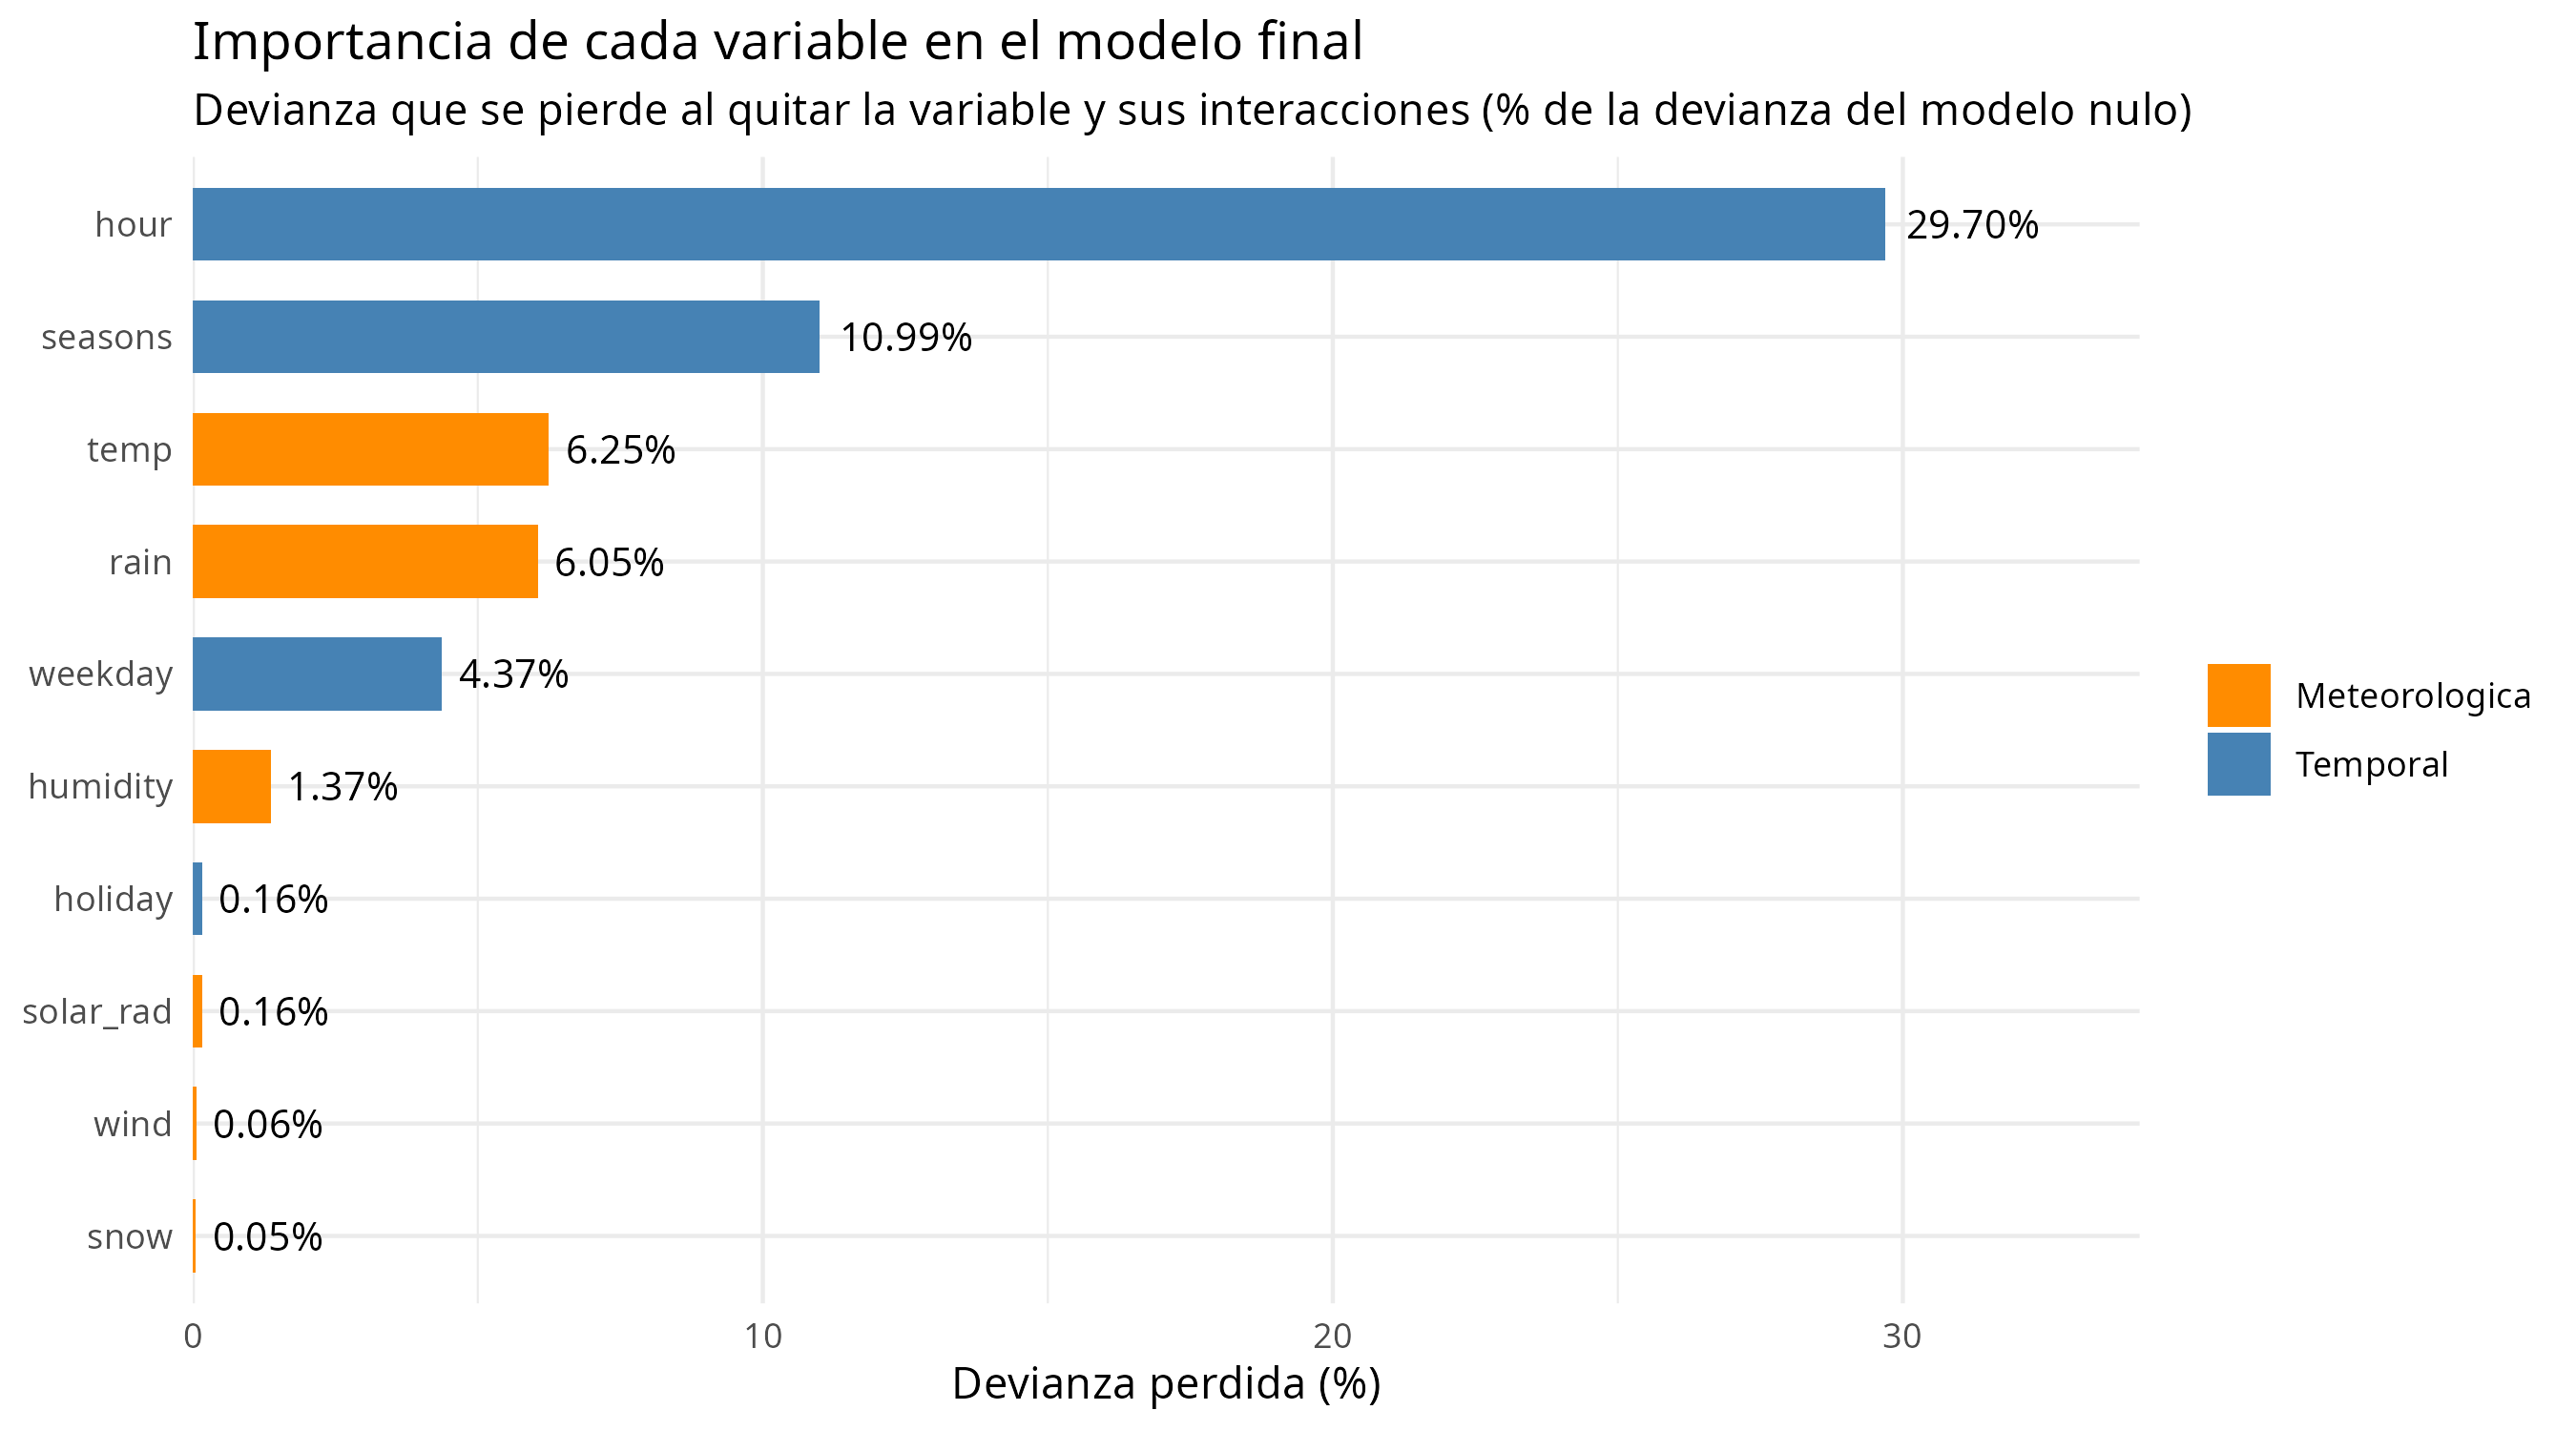
\includegraphics[width=.85\textwidth]{plots/03_efectos_importancia_variables.png}
\caption{Devianza perdida al eliminar cada variable y sus interacciones del modelo final, como porcentaje de la devianza del modelo nulo.}
\label{fig:importancia}
\end{figure}

La hora del día es, por amplio margen, la variable más importante ($29{,}70\%$), seguida de la estación del año ($10{,}99\%$), la temperatura ($6{,}25\%$), la lluvia ($6{,}05\%$) y el día de la semana ($4{,}37\%$). La humedad tiene un aporte menor ($1{,}37\%$), mientras que el feriado ($0{,}16\%$), la radiación solar ($0{,}16\%$), el viento ($0{,}06\%$) y la nieve ($0{,}05\%$) tienen un aporte marginal. En conjunto, las variables temporales (hora, estación y día de la semana) explican la mayor parte de la variabilidad de la demanda, y entre las meteorológicas destacan la temperatura y la lluvia.

\paragraph{Efectos de las variables con interacciones.}
Como la temperatura, la lluvia y la hora participan en interacciones, sus efectos no pueden leerse directamente de un único coeficiente. Por ello se calcularon efectos promedio a partir de las predicciones del modelo: se modifica una sola variable, manteniendo todas las demás en sus valores observados, y se compara el promedio de las predicciones resultantes con el promedio de las predicciones originales. De este modo, el efecto incluye todas las interacciones de la variable.

\textit{Temperatura.} Un aumento de $5\,^\circ$C en todas las horas multiplica la demanda esperada por $1{,}303$ en primavera, $1{,}254$ en invierno y $1{,}159$ en otoño, es decir, aumentos de $30\%$, $25\%$ y $16\%$, respectivamente. En verano, en cambio, la multiplica por $0{,}831$, lo que corresponde a una disminución del $17\%$. Según la franja horaria, el efecto de $+5\,^\circ$C es mayor en la noche (21--23 h: $+14\%$; 0--5 h: $+11\%$) y en la tarde (17--20 h: $+11\%$), y menor en la mañana (6--9 h: $+2\%$), cuando gran parte de los viajes corresponde a desplazamientos obligados al trabajo o a clases. La Figura~\ref{fig:temp_estacion} muestra la demanda esperada según la temperatura dentro del rango observado en cada estación: en otoño, primavera e invierno crece con la temperatura, mientras que en verano disminuye desde cerca de $1\,468$ arriendos por hora a $18{,}6\,^\circ$C hasta cerca de 765 a $35{,}9\,^\circ$C.

\begin{figure}[htbp]
\centering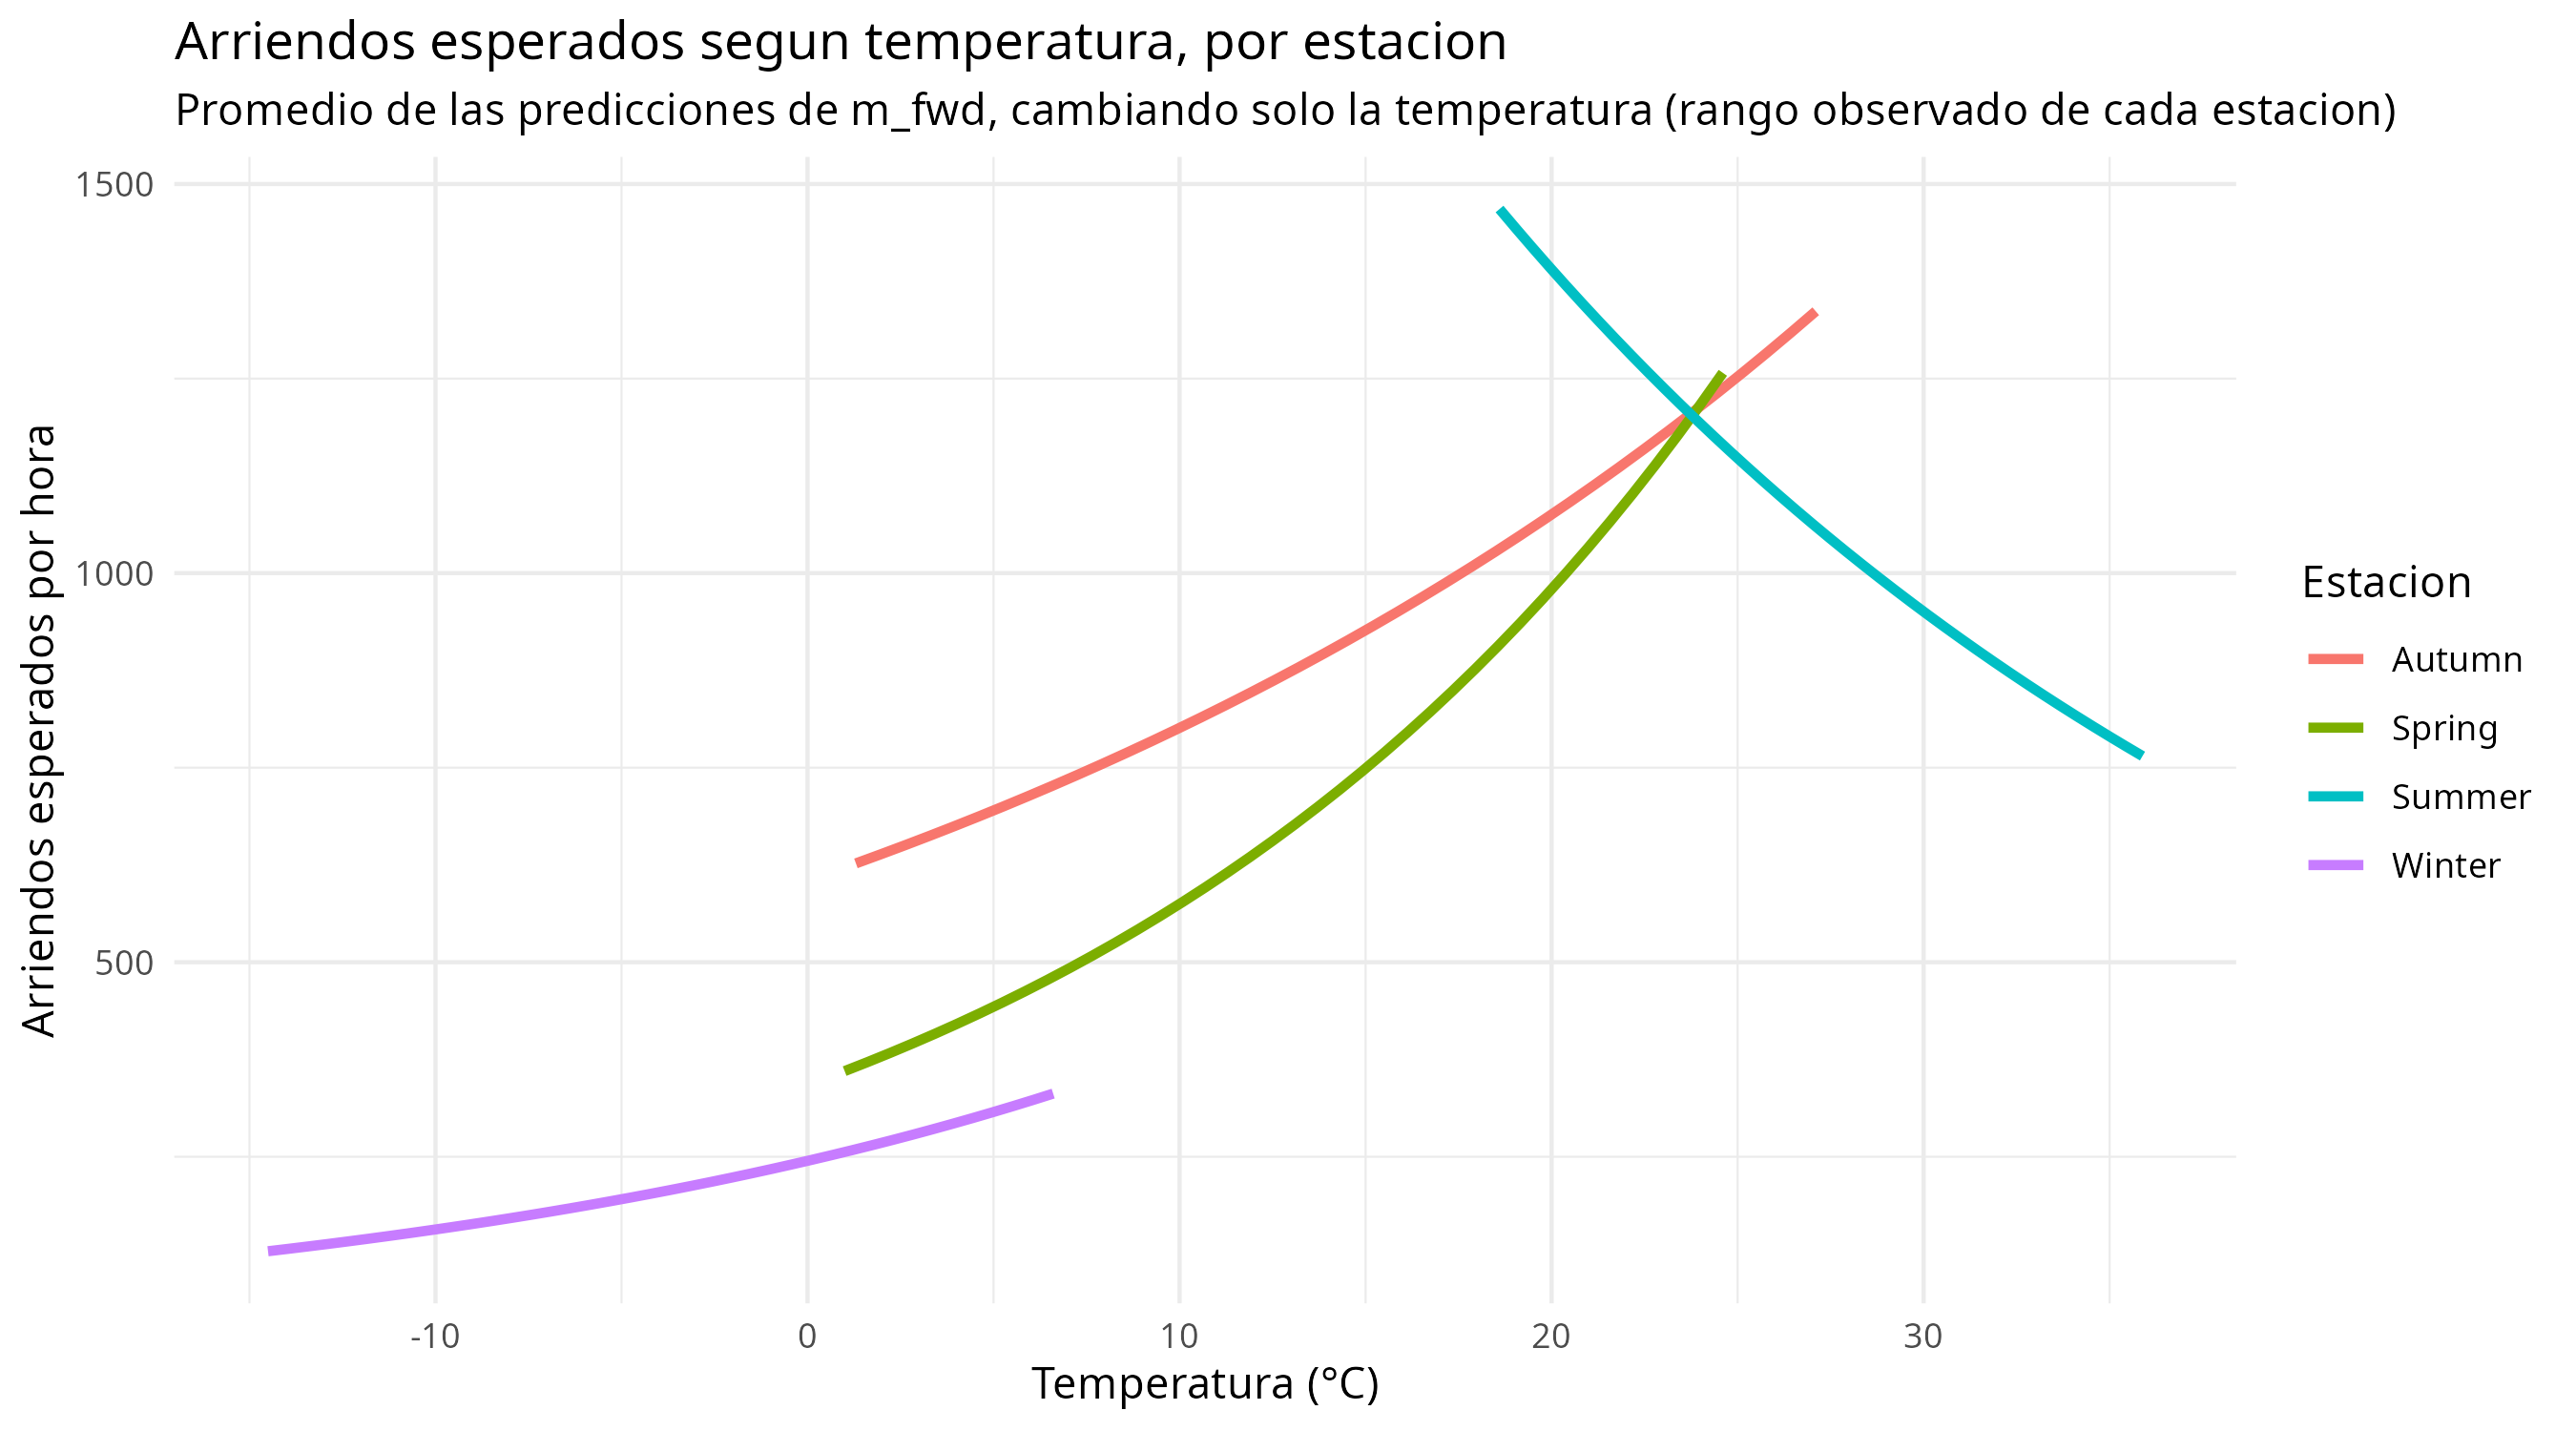
\includegraphics[width=.85\textwidth]{plots/03_efectos_temperatura_por_estacion.png}
\caption{Arriendos esperados según la temperatura en cada estación, dentro del rango observado (percentiles 2{,}5 a 97{,}5) de cada una.}
\label{fig:temp_estacion}
\end{figure}

\textit{Lluvia.} Como la lluvia interactúa con la humedad y casi no se registran horas con lluvia y humedad baja (solo 8 de las 516 horas con lluvia tienen humedad menor o igual a $57\%$), su efecto se evaluó únicamente en las horas en que efectivamente llovió, comparando la predicción observada con la que se obtendría en esas mismas horas sin lluvia. En esas horas, cuya humedad mediana es $94\%$, la lluvia multiplica la demanda esperada por $0{,}225$, es decir, la reduce en aproximadamente un $77{,}5\%$. Este resultado es coherente con los promedios observados de 167 arriendos por hora con lluvia y 766 sin lluvia.

\textit{Hora y día de la semana.} La Figura~\ref{fig:perfil_horario} muestra el perfil horario predicho para días hábiles y fines de semana. En días hábiles se observan dos máximos marcados, a las 08:00 (1306 arriendos por hora) y a las 18:00 (1724), coherentes con los desplazamientos al trabajo o a clases. En fines de semana el máximo de la mañana desaparece (421 arriendos a las 08:00) y la demanda se concentra al mediodía y en la tarde, superando a la de los días hábiles entre las 10:00 y las 16:00 (por ejemplo, 1023 frente a 790 a las 15:00). En consecuencia, el día de la semana no solo cambia el nivel de la demanda, sino sobre todo la forma de su perfil diario.

\begin{figure}[htbp]
\centering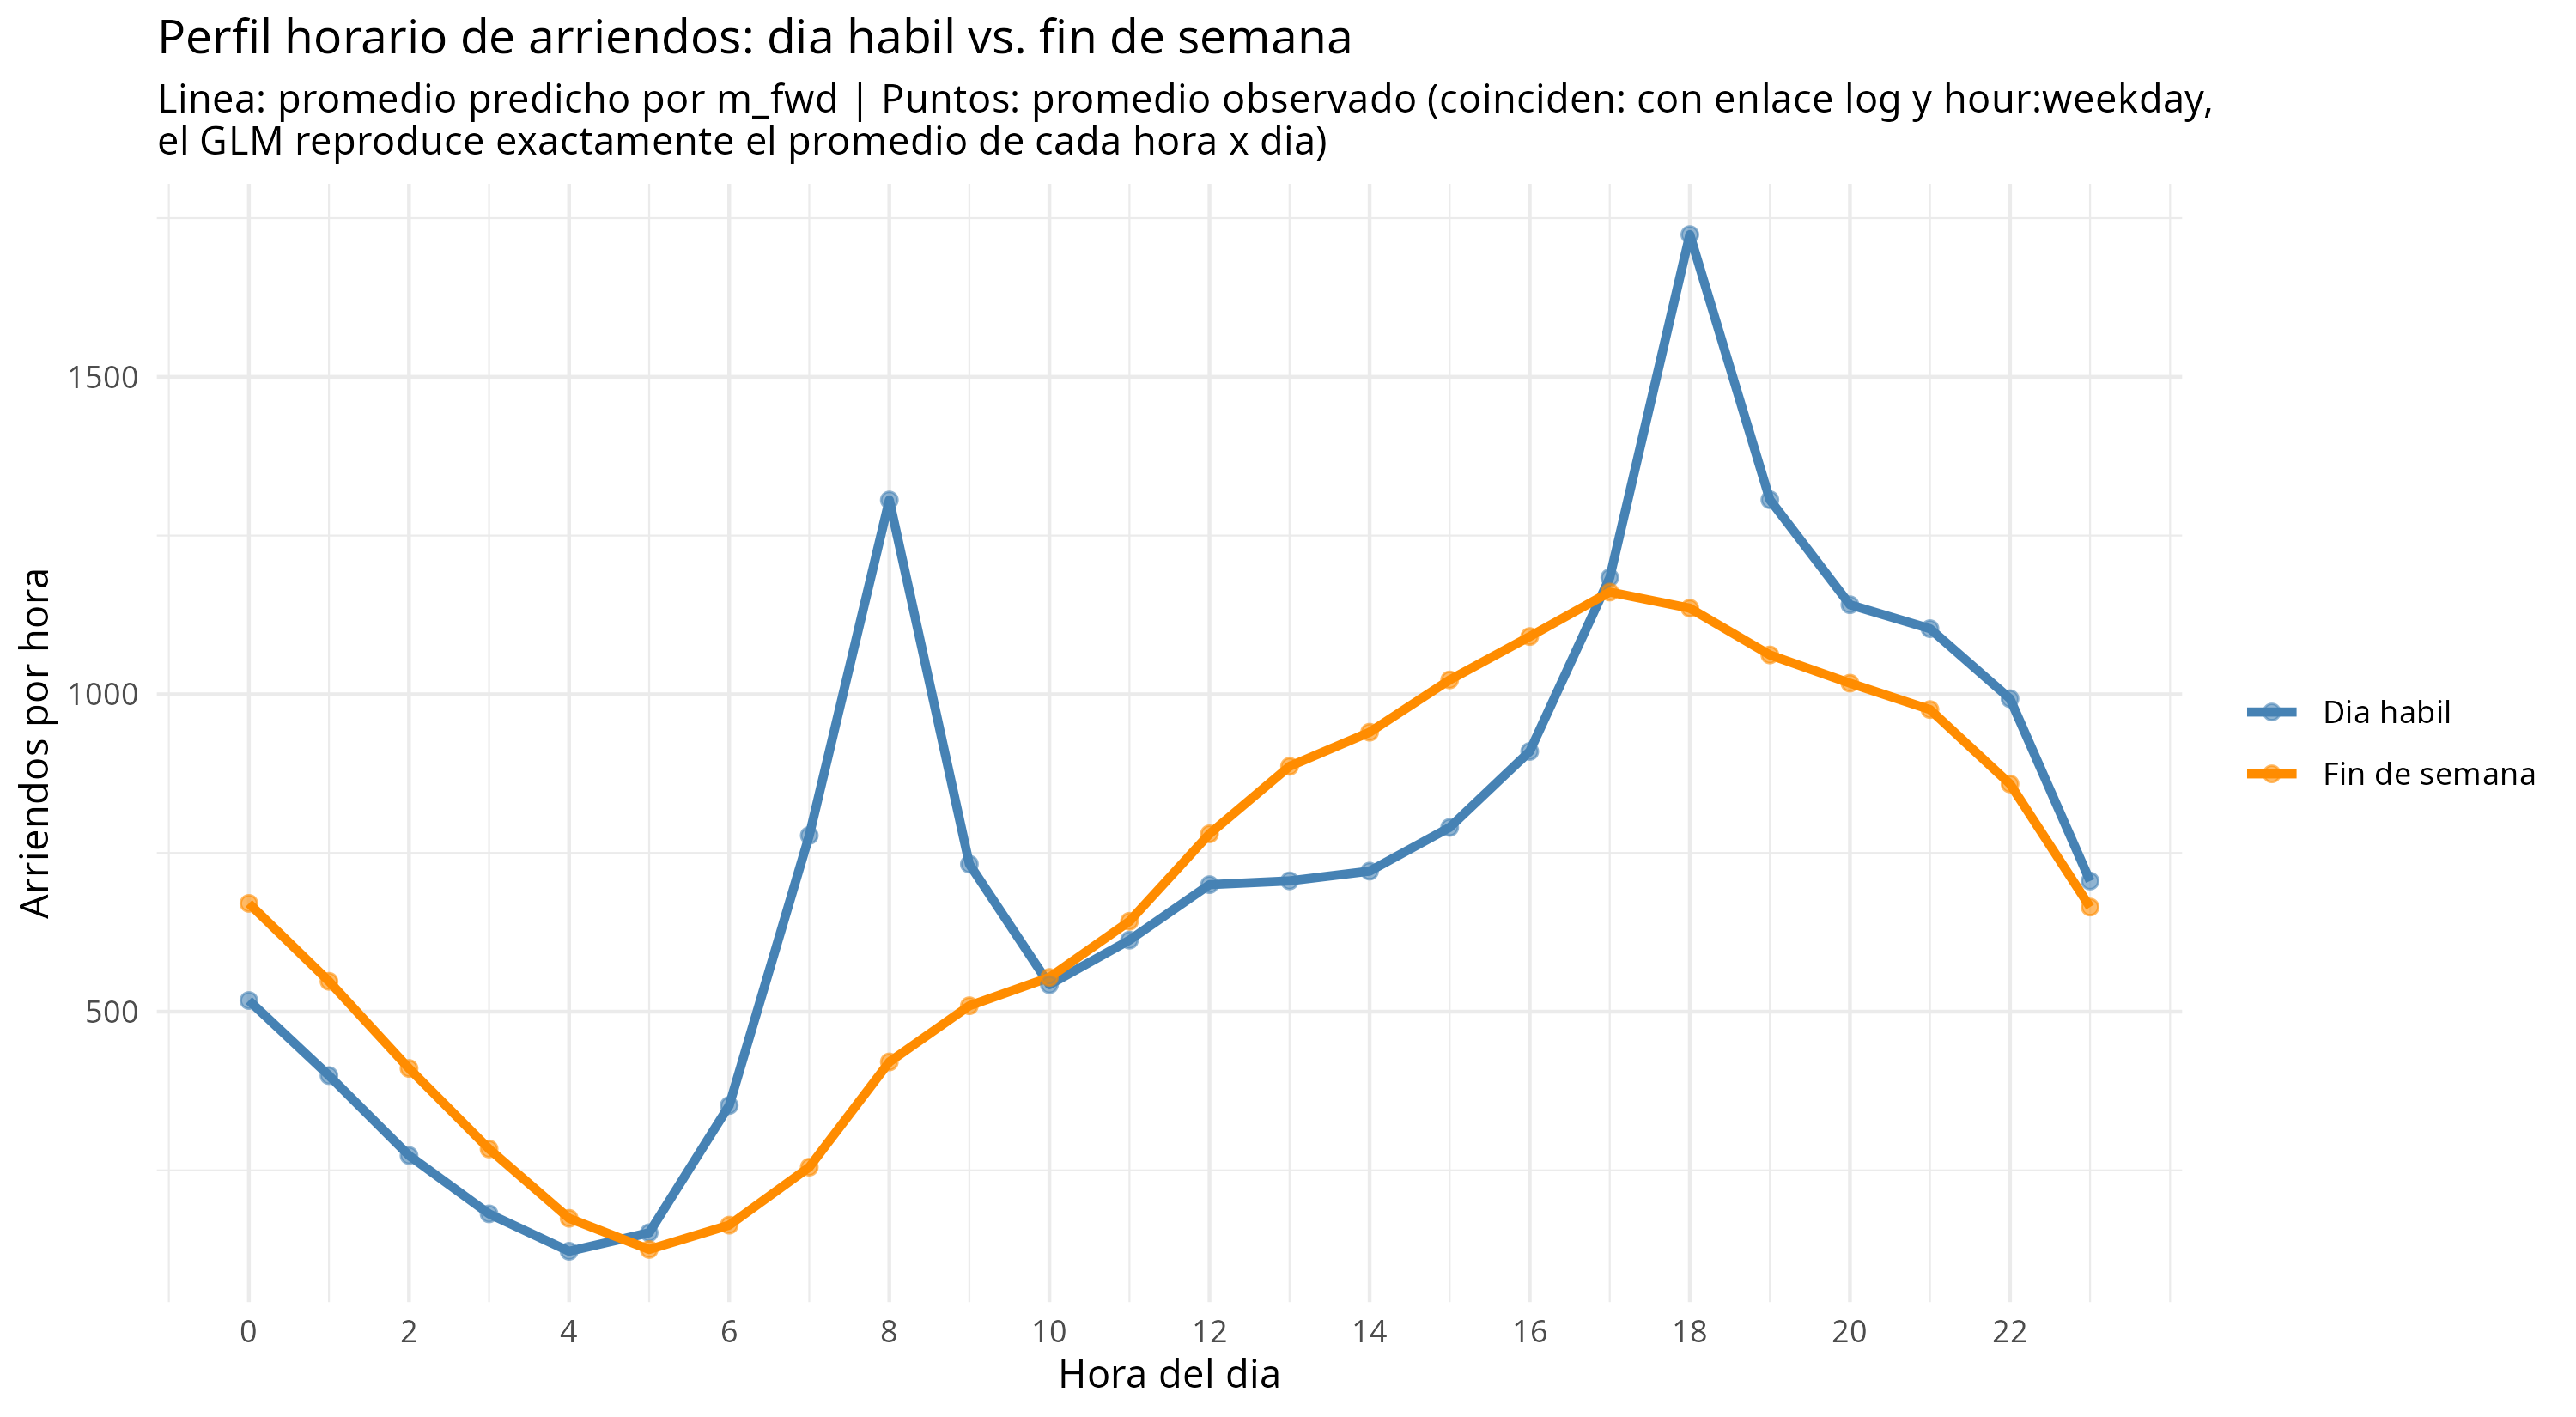
\includegraphics[width=.9\textwidth]{plots/03_efectos_perfil_horario.png}
\caption{Perfil horario de arriendos en días hábiles y fines de semana. Líneas: promedio predicho por el modelo final; puntos: promedio observado.}
\label{fig:perfil_horario}
\end{figure}

\textit{Estación.} La demanda promedio predicha es de 1034 arriendos por hora en verano, 924 en otoño, 746 en primavera y 226 en invierno, por lo que en invierno la demanda esperada es aproximadamente 4{,}6 veces menor que en verano. Estos promedios coinciden con los observados en el análisis exploratorio, ya que, con enlace logarítmico y la estación como factor, el modelo reproduce exactamente la media observada de cada estación.

\paragraph{Respuesta.}
La demanda horaria de bicicletas en Seúl está determinada principalmente por factores temporales. La hora del día es el factor más importante y su efecto depende del tipo de día: en días hábiles predominan los máximos asociados a los desplazamientos al trabajo o a clases, mientras que en fines de semana el uso se concentra al mediodía y en la tarde. La estación del año también es determinante, con una demanda invernal muy inferior a la del resto del año. Entre las condiciones climáticas, la lluvia es la que produce el mayor efecto puntual, al reducir la demanda esperada en cerca de un $78\%$ en las horas en que ocurre, mientras que la temperatura aumenta la demanda en otoño, invierno y primavera, pero la reduce en verano. La humedad, la radiación solar, el viento, la nieve y los feriados tienen un aporte comparativamente menor. Estas conclusiones se basan en la magnitud de los efectos estimados y en un modelo cuya capacidad predictiva fue validada en días no utilizados en el ajuste, y no en los valores-$p$, que no son confiables debido a la autocorrelación de los residuos.

\bigskip
\newpage

\textbf{Pregunta secundaria:}
¿De qué manera la estación del año y la franja horaria
modulan el efecto marginal de la temperatura sobre
los arriendos de bicicletas?

Para responder esta pregunta, se consideran los términos
del predictor lineal del modelo final asociados a la
temperatura. En particular, debido a las interacciones
temperatura--estación y temperatura--hora, la pendiente
asociada a la temperatura depende de la estación $j$
y de la hora $h$ consideradas.

Dicha pendiente está dada por

\[
b_{jh}=\beta_T+a_j+c_h,
\]

donde:

\begin{itemize}
    \item $\beta_T$ corresponde al coeficiente asociado
    al efecto principal de la temperatura.

    \item $a_j$ corresponde al coeficiente de interacción
    entre la temperatura y la estación $j$.

    \item $c_h$ corresponde al coeficiente de interacción
    entre la temperatura y la hora $h$.
\end{itemize}

Para las categorías de referencia, correspondientes
a otoño y a las 00:00 horas, se tiene $a_j=0$ y $c_h=0$,
respectivamente.

Dado que el modelo cuasi-Poisson utiliza una función
de enlace logarítmica, se cumple que

\[
\log(\mu_i)=\eta_i,
\qquad
\mu_i=\exp(\eta_i).
\]

Por lo tanto, el efecto marginal de la temperatura
sobre el logaritmo de la demanda esperada está dado por

\[
\frac{\partial\log(\mu_i)}{\partial T_i}
=\beta_T+a_j+c_h=b_{jh}.
\]

Aplicando la regla de la cadena, se obtiene el efecto
marginal sobre la demanda esperada en su escala original:

\[
\frac{\partial\mu_i}{\partial T_i}
=
\mu_i(\beta_T+a_j+c_h).
\]
\newpage
Esta expresión representa la tasa de cambio instantánea
de la cantidad esperada de bicicletas arrendadas respecto
de la temperatura. Su magnitud depende tanto de la
pendiente $b_{jh}$ como de la demanda esperada $\mu_i$.

Para facilitar la interpretación y comparación entre
las distintas estaciones y horas del día, se considera
la razón de medias esperadas ante un aumento de un
grado Celsius, manteniendo constantes las demás
covariables.

Esta razón está dada por

\begin{align*}
\frac{\mu(T_i+1)}{\mu(T_i)}
&=\frac{\exp(\eta_i+b_{jh})}
        {\exp(\eta_i)}\\
&=\exp(b_{jh})\\
&=\exp(\beta_T+a_j+c_h).
\end{align*}

El factor exponencial $\exp(b_{jh})$ representa el
factor multiplicativo por el cual cambia la demanda
esperada ante un aumento de un grado Celsius,
para una estación y hora determinadas.

En particular:

\begin{itemize}
    \item Si $\exp(b_{jh})>1$, la demanda esperada
    aumenta al incrementar la temperatura.

    \item Si $\exp(b_{jh})<1$, la demanda esperada
    disminuye al incrementar la temperatura.

    \item Si $\exp(b_{jh})=1$, la demanda esperada
    permanece constante ante dicho incremento.
\end{itemize}

En consecuencia, utilizando las estimaciones de los
coeficientes del modelo final, la variación porcentual
estimada de la demanda esperada se calcula mediante

\[
\Delta_{\%}(j,h)
=
100\left[
\exp(\widehat{\beta}_T+\widehat{a}_j+
\widehat{c}_h)-1
\right].
\]

Esta cantidad representa el cambio porcentual exacto
de la demanda esperada ante un incremento de un grado
Celsius, bajo la especificación del modelo.

Se calculó esta cantidad para las 96 combinaciones
posibles entre las cuatro estaciones del año y las
24 horas del día. La Tabla~\ref{tab:conclusion_temperatura}
presenta los resultados correspondientes a algunas
horas representativas.

\begin{table}[htbp]
\centering
\caption{Variación porcentual estimada de la demanda
esperada ante un aumento de $1\,^\circ$C.}
\label{tab:conclusion_temperatura}
\begin{tabular}{lrrrr}
\toprule
Hora & Otoño & Primavera & Verano & Invierno \\
\midrule
00:00 & 4{,}31 & 6{,}83 & $-$2{,}58 & 6{,}12 \\
06:00 & 3{,}35 & 5{,}85 & $-$3{,}47 & 5{,}14 \\
08:00 & 1{,}28 & 3{,}73 & $-$5{,}41 & 3{,}03 \\
12:00 & 1{,}79 & 4{,}25 & $-$4{,}93 & 3{,}55 \\
18:00 & 3{,}03 & 5{,}52 & $-$3{,}78 & 4{,}81 \\
20:00 & 4{,}88 & 7{,}41 & $-$2{,}05 & 6{,}69 \\
23:00 & 4{,}55 & 7{,}08 & $-$2{,}35 & 6{,}36 \\
\bottomrule
\end{tabular}
\end{table}
\newpage
\paragraph{Ejemplo:}

Para la primavera a las 20:00 horas, se obtuvo una
pendiente estimada de

\[
\widehat{b}_{jh}=0{,}07150.
\]

Por lo tanto, la razón de medias estimada es

\[
\exp(0{,}07150)\approx 1{,}0741.
\]

Esto significa que, ante un aumento de un grado Celsius,
la demanda esperada se multiplica aproximadamente
por $1{,}0741$, manteniendo constantes las demás
covariables.

Equivalentemente, la variación porcentual está dada por

\[
100(1{,}0741-1)=7{,}41\%.
\]

Por consiguiente, durante la primavera a las 20:00 horas,
un aumento de un grado Celsius se asocia con un
incremento estimado del $7{,}41\%$ en la cantidad
esperada de bicicletas arrendadas.

En contraste, para el verano a las 08:00 horas,
se obtuvo una pendiente estimada de

\[
\widehat{b}_{jh}=-0{,}05558.
\]

La razón de medias correspondiente es

\[
\exp(-0{,}05558)\approx 0{,}9459.
\]

En este caso, la demanda esperada se multiplica por
$0{,}9459$, lo que equivale a una disminución de

\[
100(0{,}9459-1)=-5{,}41\%.
\]

\paragraph{Comparación entre estaciones.}

Durante la primavera se obtiene la mayor asociación
positiva entre la temperatura y la demanda esperada,
con incrementos estimados entre $3{,}73\%$ y $7{,}41\%$,
dependiendo de la hora del día.

En invierno, los incrementos se encuentran entre
$3{,}03\%$ y $6{,}69\%$, mientras que en otoño varían
entre $1{,}28\%$ y $4{,}88\%$.

En contraste, durante el verano se observa una
asociación negativa para las 24 horas del día,
con disminuciones estimadas entre $2{,}05\%$ y
$5{,}41\%$ ante un aumento de un grado Celsius.

Una posible explicación de este comportamiento es que,
durante las estaciones más frías, un aumento de la
temperatura podría generar condiciones más favorables
para utilizar bicicletas, mientras que durante el
verano las temperaturas elevadas podrían desincentivar
su utilización.

Sin embargo, esta explicación constituye una
interpretación contextual y no una relación causal
demostrada por el modelo.

\paragraph{Comparación entre horas del día.}

A las 08:00 horas se obtiene la menor variación
porcentual estimada en todas las estaciones.
En otoño, primavera e invierno esto corresponde
al menor incremento porcentual, mientras que
en verano corresponde a la mayor disminución.

Por otra parte, a las 20:00 horas se obtiene
la mayor variación porcentual estimada en todas
las estaciones. En verano, esto corresponde a
la menor disminución de la demanda esperada.

Por consiguiente, bajo la especificación del modelo,
la estación del año modifica tanto la magnitud como
el signo de la asociación entre la temperatura y
la demanda esperada, mientras que la hora del día
modifica su magnitud dentro de cada estación.

Estos resultados permiten comprender la importancia
de incorporar las interacciones temperatura--estación
y temperatura--hora, puesto que un modelo aditivo
impondría una misma variación porcentual de la
demanda ante cambios de temperatura, independientemente
de la estación y la hora consideradas.

\subsection{Limitaciones y posibles extensiones}

La principal limitación del modelo es la autocorrelación
temporal de los residuos, puesto que el modelo cuasi-Poisson
permite considerar la sobredispersión, pero no la dependencia
entre observaciones. Si bien el parámetro de dispersión
disminuyó de $104{,}89$ a $50{,}89$, la sobredispersión sigue
siendo considerable.

Debido a la dependencia temporal, los resultados se
interpretan desde una perspectiva descriptiva, sin recurrir
a pruebas de significancia estadística. Asimismo, aunque
la validación cruzada muestra una mejora en la capacidad
predictiva, esta no garantiza la ausencia de sobreajuste.

Como posibles extensiones, se propone incorporar estructuras
de dependencia temporal, estudiar relaciones no lineales
entre las covariables y la demanda, y buscar modelos más
parsimoniosos que permitan conservar la calidad del ajuste
y la capacidad predictiva.
\newpage
\FloatBarrier
\section{Declaración de uso de herramientas de inteligencia artificial}\label{sec:ia}
En la elaboración del presente informe se utilizaron
herramientas de inteligencia artificial como apoyo al
desarrollo de la tarea. Se utilizó Gemini (Google, 2026) \cite{google}
para estructurar la plantilla base sobre la cual se desarrolló posteriormente el informe, lo que afectó a las secciones 1 a 6. Esta plantilla fue validada por nosotros, verificando su correcta visualización y que contuviera las secciones y subsecciones relevantes que trataríamos en este trabajo. Además, se utilizó para la búsqueda de referencias bibliográficas con las que apoyar las decisiones metodológicas, lo que afectó principalmente a las secciones de referencias y metodología. Esto fue validado mediante la consulta al libro de texto sugerido y la revisión de la teoría. Por otra parte, se utilizó Claude
(Anthropic, 2026) \cite{anthropic} para asistir en la implementación, revisión y corrección de los códigos en R anexos empleados en el análisis estadístico.

Asimismo, se utilizó ChatGPT (OpenAI, 2026) \cite{openai} como apoyo
en la formulación del apartado de Resultados, tanto en la interpretación de los resultados como en la
redacción, la generación de tablas y la organización del informe en \LaTeX. Esto fue validado revisando que lo declarado en el informe se condijera con el desarrollo del código y verificando la correcta visualización de las tablas.

La revisión de los códigos, la verificación de los
resultados y la interpretación final del análisis
son responsabilidad de los autores.

\begin{thebibliography}{99}
\bibitem{dunn} Dunn, P. K., \& Smyth, G. K. (2018). \textit{Generalized Linear Models With Examples in R}. Springer.
\bibitem{fox} Fox, J., \& Monette, G. (1992). Generalized collinearity diagnostics. \textit{Journal of the American Statistical Association}, 87(417), 178--183.
\bibitem{mccullagh} McCullagh, P., \& Nelder, J. A. (1989). \textit{Generalized Linear Models} (2nd ed.). Chapman \& Hall.
\bibitem{roberts} Roberts, D. R., et al. (2017). Cross-validation strategies for data with temporal, spatial, hierarchical, or phylogenetic structure. \textit{Ecography}, 40(8), 913--929.
\bibitem{sathish} Sathishkumar, V. E., Park, J., \& Cho, Y. (2020). Using data mining techniques for bike sharing demand prediction in metropolitan city. \textit{Computer Communications}, 153, 353--366.
\bibitem{venables} Venables, W. N., \& Ripley, B. D. (2002). \textit{Modern Applied Statistics with S} (4th ed.). Springer.
\bibitem{verhoef} Ver Hoef, J. M., \& Boveng, P. L. (2007). Quasi-Poisson vs. negative binomial regression: How should we model overdispersed count data? \textit{Ecology}, 88(11), 2766--2772.
\bibitem{google} Google (2026). Gemini [Modelo de lenguaje de gran escala].
\bibitem{openai} OpenAI (2026). ChatGPT [Modelo de lenguaje de gran escala].
\bibitem{anthropic} Anthropic (2026). Claude [Modelo de lenguaje de gran escala].
\end{thebibliography}

\end{document}